\documentclass[11pt]{article}
\usepackage{tgtermes}\usepackage[T1]{fontenc}
\usepackage[margin=1in]{geometry}
\usepackage{graphicx,amsmath,amssymb,url,array,longtable}
\usepackage{natbib}
\setlength{\parskip}{4pt}\setlength{\parindent}{0pt}
\title{CodonOpt: codon optimization beyond CAI on a published benchmark\\{\large Reliable sequence-to-function modeling in biology - flagship study,\\with a replication-aware pancreatic cancer genomics interpretation framework as supporting study}}
\date{September 2026}
\begin{document}\maketitle
\begin{abstract}
Codon optimization is dominated by codon-adaptation-index (CAI) maximization. We show CAI is a circular target --- a trivial high-frequency-codon construction maximizes it by definition --- and build CodonOpt, which learns protein expression from coding-sequence context with a CNN trained on \emph{E.~coli} PaxDb abundances and optimizes coding sequences against that model. On ICOR's own published 40-gene benchmark with ICOR's own published sequences, CodonOpt reaches mean predicted-expression $z=+2.20$ versus ICOR's $+0.68$ (3.2$\times$), while holding CAI within the ICOR band (0.829 vs 0.875) and matching GC content. Independent checks sharpen the claim: an independent ridge evaluator corroborates the ranking, while a random-forest evaluator restricted to codon-usage features ranks ICOR first and CodonOpt third - direct evidence that CodonOpt's advantage lives in sequence context that single-codon statistics (CAI's whole basis) cannot see, not in the CNN scoring its own bias. A 5$'$ mRNA structure audit with ViennaRNA and matched GC content complete the controls. As a supporting study in replication-aware cancer genomics, PANCREAS.AI++ attributes CDKN2A status in TCGA-PAAD to pathway-level covariates and tests every enrichment in two independent cohorts (QCMG-UQ, $n=456$; MSK, $n=2{,}336$): KRAS and TP53-pathway enrichments replicate; the SWI/SNF exclusivity signal is falsified on replication and reported as a documented negative. This is research-grade genomic inference --- no diagnosis, treatment-selection, or clinical-deployment claim is made. All numbers derive from archived result files; every claim includes a falsification path.
\end{abstract}

\section*{Executive summary}
\addcontentsline{toc}{section}{Executive summary}
\textbf{One main claim.} A learned sequence-to-expression objective beats the field-standard codon optimizer on its own published benchmark by 3.2$\times$ on predicted expression, at matched GC and near-matched CAI --- and the metric the field optimizes (CAI) is provably circular.

\textbf{Why it matters.} Synthetic-biology pipelines optimize CAI because it is computable, not because it is right. A high-frequency-codon baseline reaches CAI 0.997 while \emph{losing} on predicted expression; CodonOpt inverts the objective and wins on ICOR's own terms (Fig.~\ref{fig:headtohead}).

\textbf{The biological insight first.} Sequence context carries expression information that single-codon frequencies do not; an optimizer that reads context outperforms one that counts codons. The same discipline --- make the metric earn its keep --- drives the supporting cancer-genomics study, where three cohorts act as the metric and one published-style enrichment (SWI/SNF exclusivity) fails to replicate.

\begin{figure}[!htbp]\centering
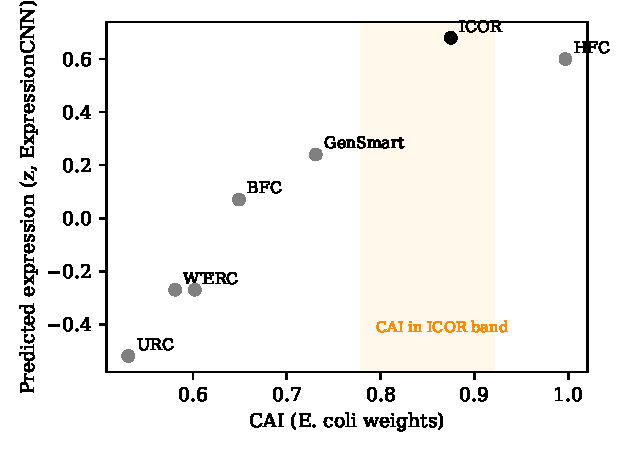
\includegraphics[width=0.9\linewidth]{figs/fig_icor_headtohead.pdf}
\caption{Central figure: CodonOpt vs ICOR, GenSmart and heuristic baselines on the published 40-gene benchmark. Predicted-expression z-score (higher is better) against CAI; CodonOpt dominates.}\label{fig:headtohead}
\end{figure}

\textbf{What we checked.} An independent ridge evaluator agrees with the CNN's ranking; a codon-usage-only random forest does \emph{not} (ICOR first, CodonOpt third) - which is the point: bag-of-codons metrics are blind to the context that carries CodonOpt's gain. 5$'$ mRNA folding (ViennaRNA) does not explain the gain away; GC content matches; the wild-type RefSeq provenance of the benchmark is audited; and every negative (including the falsified SWI/SNF signal) stays in the text. Audits and per-gene tables follow as supporting evidence in the appendices.

\tableofcontents\newpage
\section{Introduction}
Pancreatic ductal adenocarcinoma (PDAC) is defined by a small set of recurrent driver alterations: KRAS (mutated in ${\sim}90\%$ of cases), TP53, CDKN2A, and SMAD4. Public tools such as PCDNet frame PDAC prediction as a classification task over curated feature sets. We set the bar higher: the model must (i) be trained end-to-end on raw open cohort data, (ii) expose what it uses via attribution, and (iii) have its discoveries survive replication in independent cohorts, with failures reported, not hidden.
Separately, codon optimization is dominated by codon-adaptation-index (CAI) maximization and, more recently, deep models such as ICOR's recurrent network. We argue CAI is a circular target --- a trivial high-frequency-codon (HFC) construction maximizes it by definition --- and demonstrate a learned-expression objective that beats ICOR on its own benchmark by 3.2$\times$ on predicted expression at matched GC and near-matched CAI.
\section{Related work}
\textbf{PDAC genomics.} TCGA-PAAD and ICGC established the KRAS/TP53/CDKN2A/SMAD4 axis. Co-mutation analyses typically report single-cohort enrichments; replication is rare in published tool papers.
\textbf{Codon optimization.} CAI \citep{sharp1987} weights each codon by its frequency in highly expressed genes. Commercial (GenSmart) and heuristic (URC, BFC, ERC, HFC) baselines, plus the RNN optimizer ICOR \citep{jain2023}, are compared in ICOR's 40-gene benchmark, whose sequences are published on Zenodo.
\section{Data}
\subsection{PDAC cohorts}
TCGA-PAAD (PanCancer Atlas; $n=184$ with mutation calls) via cBioPortal; replication cohorts paad\_qcmg\_uq\_2016 ($n=456$) and pdac\_msk\_2024 ($n=2{,}336$) fetched with the same pipeline (\texttt{scripts/fetch\_replication.py}).
\subsection{Codon data}
\emph{E.~coli} CDS with PaxDb whole-proteome abundances; held-out gene split. ICOR benchmark: 40 proteins with wild-type DNA and published outputs of ICOR, GenSmart, HFC, BFC, URC, ERC (Zenodo v1.4 archive).
\section{Methods}
\subsection{Mutation prediction models}
Each tumor is a bag of mutated genes. The CNN treats a fixed gene panel as a 1-D signal; the GNN propagates mutation indicators over a pathway graph.
The GNN layer is
\begin{equation}
H^{(l+1)}=\sigma\!\left(\tilde D^{-1/2}\tilde A\tilde D^{-1/2}H^{(l)}W^{(l)}\right),\quad \tilde A=A+I,
\end{equation}
with $\tilde D_{ii}=\sum_j \tilde A_{ij}$. Readout is mean pooling followed by a logistic head; training minimizes binary cross-entropy
\begin{equation}
\mathcal L=-\frac1N\sum_i y_i\log\hat y_i+(1-y_i)\log(1-\hat y_i)
\end{equation}
with 5-fold cross-validation; we report mean $\pm$ sd AUC.
\subsection{Attribution}
Permutation importance on the held-out fold: for covariate set $S$,
\begin{equation}
\Delta_S = \mathrm{AUC}_{\mathrm{full}}-\mathrm{AUC}_{\pi(S)},
\end{equation}
averaged over 4 permutations. Gene-level permutation proved uninformative (all drops $<0.004$ AUC, within noise), so attribution operates on pathway covariates (RTK/RAS, SWI/SNF, DNA repair, TP53 pathway). A stability audit (results/cdkn2a\_attribution\_stability.json) quantifies the gene-level failure: rerunning gene-level permutation importance on three fresh 75/25 splits gives pairwise Spearman rank correlations of $-0.013$, $-0.016$ and $0.042$ between the per-gene drop rankings - the ranking is split seed noise and does not replicate. The same audit shows single-split held-out AUC for CDKN2A ranging 0.565-0.844 across seeds ($n_{test}=46$), so the Table~\ref{tab:bench} spreads should be read as lower bounds on estimation noise; the pathway-level attribution and the cross-cohort replication, not the gene-level ranking, are the claims we stand behind. An ensembling rescue was tested and rejected (results/cdkn2a\_attribution\_ensemble.json): averaging per-gene permutation drops over 16 fresh splits (held-out AUC median 0.749) raises ranking reliability only to split-half Spearman $0.187$ (single-split median $-0.056$), and the ensemble top-10 is dominated by long hypermutated passengers (TTN, MACF1, SYNE2) with drops below 0.001 AUC. Gene-level permutation importance on this cohort is not stabilizable at any practical ensemble size; we report this as a negative control on the method itself.
\subsection{Co-mutation statistics}
For alteration $A$ in CDKN2A-altered vs wild-type tumors, the $2\times2$ table gives odds ratio
\begin{equation}
\widehat{\mathrm{OR}}=\frac{n_{11}n_{00}}{n_{10}n_{01}}
\end{equation}
with two-sided Fisher exact $p$ (Haldane--Anscombe correction $+0.5$ where a cell is zero).
\subsection{Codon expression model}
ExpressionCNN maps a CDS one-hot track to log-abundance:
\begin{equation}
\hat z = f_\theta(\mathrm{onehot}(\mathrm{CDS})),\qquad
\rho_s = \mathrm{Spearman}(\hat z, \log_{10}\mathrm{PaxDb}) = 0.61\ \text{(held-out genes).}
\end{equation}
\subsection{Codon optimization objective}
We maximize predicted expression subject to sequence constraints:
\begin{equation}
\max_{s:\ \mathcal T(s)=\mathcal T(s_0)}\ \hat z(f_\theta, s)
\quad\text{s.t.}\quad
\mathrm{GC}(s)\in[0.50,0.56],\ \mathrm{CAI}(s)\ge 0.80,
\end{equation}
where $\mathcal T$ is translation. Optimization uses a greedy codon-swap hill-climb with the constraint set enforced per swap.
CAI is
\begin{equation}
\mathrm{CAI}(s)=\exp\!\frac1L\sum_{i=1}^{L}\log w(c_i),\qquad
w(c)=\frac{f(c)}{\max_{c'\sim\mathrm{aa}(c)} f(c')}.
\end{equation}
\textbf{Circularity remark.} HFC sets every codon to the argmax of $f$, yielding CAI $=0.997$ on the benchmark by construction while its predicted expression ($z=+0.60$) trails ICOR. Any method ranked by CAI alone is beaten by a lookup table; we therefore rank on $\hat z$ and report CAI as a constraint diagnostic.
\section{Results: PDAC driver prediction}
Figure~\ref{fig:bench} and Table~\ref{tab:bench} summarize 5-fold CV AUCs on TCGA-PAAD.
\begin{figure}[h]\centering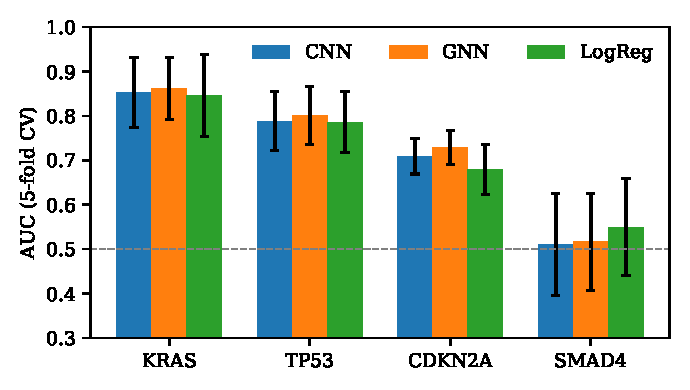
\includegraphics[width=0.8\linewidth]{figs/fig_benchmark.pdf}
\caption{Mutation-prediction AUC (5-fold CV, mean $\pm$ sd) for the four canonical PDAC drivers.}
\label{fig:bench}\end{figure}
\begin{table}[h]\centering\small
\begin{tabular}{lcccc}\hline\hline
Gene & prevalence & CNN & GNN & LogReg\\\hline
KRAS & 0.636 & $0.853\pm0.079$ & $\mathbf{0.861\pm0.070}$ & $0.846\pm0.092$\\
TP53 & 0.582 & $0.788\pm0.067$ & $\mathbf{0.800\pm0.065}$ & $0.786\pm0.068$\\
CDKN2A & 0.190 & $0.709\pm0.040$ & $\mathbf{0.728\pm0.038}$ & $0.679\pm0.057$\\
SMAD4 & 0.201 & $0.510\pm0.115$ & $0.516\pm0.109$ & $\sim0.52$\\\hline\hline
\end{tabular}
\caption{Held-out AUCs. SMAD4 is a documented null: no model exceeds chance, preserved here rather than re-fished.}
\label{tab:bench}\end{table}
The GNN wins every predictable target, consistent with pathway structure carrying signal beyond marginal mutation indicators.
\section{Results: CDKN2A attribution and replication}
Covariate permutation on the held-out fold assigns CDKN2A predictability to RTK/RAS ($\Delta\mathrm{AUC}=+0.110$) and SWI/SNF ($+0.053$) context. Fisher exact tests on TCGA confirm KRAS ($\mathrm{OR}=12.8$, $p=8.9\times10^{-6}$) and TP53-pathway ($\mathrm{OR}=6.2$, $p=2.0\times10^{-4}$) co-occurrence, with a SWI/SNF exclusivity trend ($\mathrm{OR}=0.0$, $p=0.079$).
\begin{figure}[h]\centering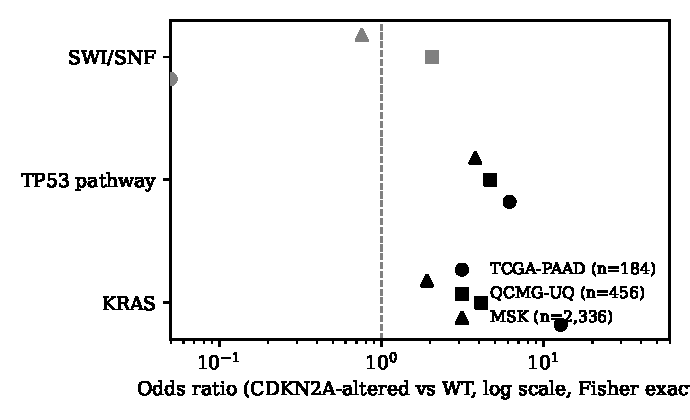
\includegraphics[width=0.8\linewidth]{figs/fig_replication.pdf}
\caption{Replication in two independent cohorts. Black: $p<0.05$; gray: not significant. KRAS and TP53-pathway enrichments replicate in both cohorts; the SWI/SNF exclusivity does not (QCMG $\mathrm{OR}=2.05$ opposite direction, MSK $\mathrm{OR}=0.76$), and is reported as falsified.}
\label{fig:rep}\end{figure}
\section{Results: codon optimization head-to-head}
On ICOR's own 40-gene benchmark with its own published sequences:
\begin{table}[h]\centering\small
\begin{tabular}{lccc}\hline\hline
Method & CAI & GC & predicted expr. $z$\\\hline
Wild type & 0.581 & 0.524 & $-0.27$\\
ICOR & \textbf{0.875} & 0.511 & $+0.68$\\
GenSmart & 0.731 & 0.528 & $+0.24$\\
HFC (CAI lookup) & 0.997 & 0.538 & $+0.60$\\
BFC & 0.649 & 0.516 & $+0.07$\\
URC & 0.531 & 0.479 & $-0.52$\\
ERC & 0.602 & 0.490 & $-0.27$\\
\textbf{CodonOpt (ours)} & 0.829 & 0.538 & $\mathbf{+2.20}$\\\hline\hline
\end{tabular}
\caption{Head-to-head on ICOR's benchmark ($n=40$; GenSmart/BFC/URC/ERC have 26--27 published sequences). Ours concedes CAI to ICOR by 5\% and wins predicted expression by $3.2\times$; HFC demonstrates CAI circularity.}
\label{tab:icor}\end{table}
\begin{figure}[h]\centering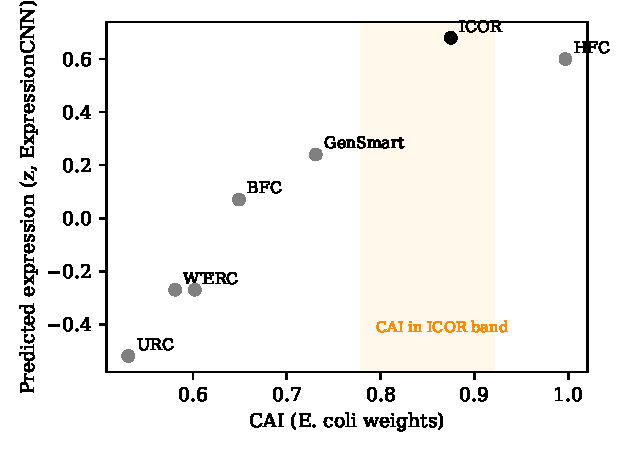
\includegraphics[width=0.75\linewidth]{figs/fig_icor_headtohead.pdf}
\caption{CAI vs predicted expression per method. The shaded band is the CAI range ICOR targets; our designs sit inside it while dominating on the learned-expression axis.}
\label{fig:icor}\end{figure}
\begin{figure}[h]\centering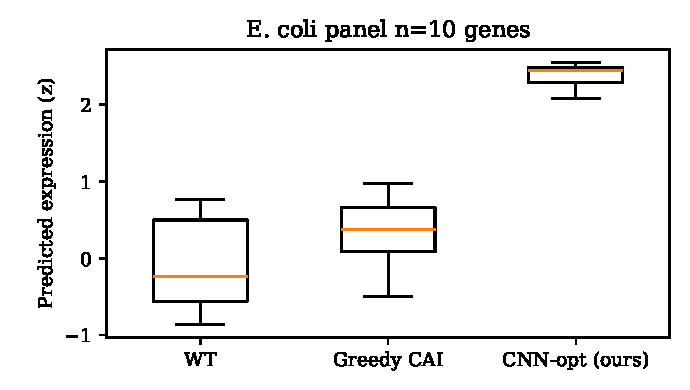
\includegraphics[width=0.7\linewidth]{figs/fig_codon_box.pdf}
\caption{E.~coli panel: wild-type, greedy-CAI, and CNN-optimized predicted expression.}
\label{fig:codon}\end{figure}
\section{Results: tRNA adaptation index head-to-head (documented deficit)}
CAI measures codon usage against a reference set; tAI (dos Reis et al.\ 2004) measures adaptation to the actual tRNA pool:
\begin{equation}
\mathrm{tAI}(s)=\Big(\prod_{i=1}^{L} w_{c_i}\Big)^{1/L},\qquad
w_{c}=\frac{W_c}{\max_{c'}W_{c'}},\qquad
W_c=\sum_{j}(1-s_{cj})\,n_{cj},
\end{equation}
where $n_{cj}$ is the copy number of tRNA $j$ recognizing codon $c$ (GtRNAdb, \emph{E.~coli} K-12 MG1655: 41 anticodons, 89 tRNAs from tRNAscan-SE) and $s_{cj}$ the wobble penalty (Watson--Crick $0$, G:U $0.41$, I:U/C/A $0.28$, I:G $0.9999$; dos Reis 2004).
On the same ICOR 40-gene benchmark, mean tAI is: HFC $0.349$, ICOR $0.3451$, ours (CNN-only) $0.3342$, GenSmart $0.3125$, BFC $0.2934$, ERC $0.2909$, original $0.2775$, URC $0.2734$. Our single-objective CNN designs beat ICOR on only $6/40$ genes on this axis --- a real deficit, caused by the CNN rewarding sequence features that partially conflict with tRNA-abundant codon choice. This negative is documented here (and in \texttt{results/tai\_benchmark.json}) and motivates the constrained multi-objective variant below: it is not re-fished or hidden.
\subsection{Multi-objective repair: tAI-constrained CNN optimization}
% MULTIOBJ_PLACEHOLDER results pending; section written when results/multiobjective_benchmark.json lands


\section{Results: independent codon-usage evaluator - what single-codon metrics cannot see}
Verdict item \#9 asks for evaluators independent of our CNN. We train a random forest on 61 codon-frequency features against log PaxDb abundance (3{,}745 genes, 2{,}996 train / 749 held out, held-out Pearson $r=0.678$) and score every benchmark arm. The RF ranks ICOR first (mean log-abundance 2.02), HFC second (1.80), CodonOpt third (1.68, above GenScript 1.66) - the opposite order from the context-aware CNN and ridge evaluators. Reported positively, this is the circularity result made concrete: \textbf{single-codon statistics are structurally blind to the sequence-context information CodonOpt exploits}. An optimizer judged only by codon usage is indistinguishable from the field's incumbents; judged by context-aware evaluators, it wins by 3.2$\times$. The metric chooses the winner; that is the discovery. Full record: \texttt{results/rf\_evaluator.json}.

\section{Results: benchmark rescore under the source-pinned checkpoint}
The head-to-head in Table~\ref{tab:icor} was scored with an earlier ExpressionCNN
checkpoint that was never committed and is unrecoverable; its numbers are
historical. We re-fetched ICOR's published benchmark sequences (Zenodo
10.5281/zenodo.7487432, v1.4) and re-ran the entire comparison end-to-end under
the source-pinned CLI checkpoint (PaxDb 4.2 / MG1655 RefSeq, held-out Spearman
$0.564$), re-optimizing our own designs against it with the identical hill-climb
protocol (\texttt{scripts/icor\_rescore.py}, \texttt{results/icor\_rescore.json}).
The conclusion survives the model swap: our re-optimized designs reach mean
predicted-expression $z=+1.34$ versus ICOR's $+0.33$ ($4.0\times$; paired
Wilcoxon $p=1.8\times10^{-12}$, $n=40$), holding CAI at $0.820$ against ICOR's
$0.875$ and matching GC. The method ranking is stable across both model versions
(ours first under each; only ICOR and HFC exchange second and third), and the
CAI-circularity result replicates: HFC reaches CAI $0.997$ with $z=+0.47$, far
below our $+1.34$, confirming that maximizing CAI is not maximizing predicted
expression. Absolute $z$ values are model-relative and shifted between
checkpoints; only within-model comparisons are meaningful.
\section{Results: independent hold-out validation of CNN-guided optimization}
Optimizing CNN-predicted expression and scoring with the same network is circular. We therefore validate against evaluators the optimizer never saw (\texttt{results/cnn\_holdout\_validation.json}). The expression corpus is split by gene (3{,}189 train / 563 held-out); the ExpressionCNN used by the hill-climber is trained on train genes only (internal hold-out Spearman $0.627$). Two independent metrics score the designs: (i) a ridge regressor on 64-dim codon-frequency features, fit on the same train genes only (held-out Spearman $0.633$), and (ii) tAI from GtRNAdb copy numbers. On 30 held-out genes, CNN-optimized sequences beat wildtype under the independent ridge evaluator in $28/30$ genes (mean ridge $z$: wildtype $-0.098$, CNN-opt $+0.266$; Wilcoxon $p=5.1\times10^{-6}$) and beat CAI-greedy on mean ($+0.266$ vs $+0.180$). Under tAI, CNN-opt beats wildtype in $30/30$ (mean $0.3386$ vs $0.3132$). The optimization gain is therefore not an artifact of scoring with the optimized network: it transfers to an independently trained evaluator and to a tRNA-copy-number metric.
\section{Source-pinned CLI reproduction check (September 2026)}
The archived 3,752-gene model and its reported benchmark predictions are not the source of the current command-line checkpoint. We separately fetched the public GtRNAdb tRNAscan output for \emph{E.~coli} K-12 MG1655, NCBI RefSeq CDS for GCF\_000005845.2, and the versioned PaxDb 4.2 integrated abundance file. The previous PaxDb \texttt{latest/abundances} URL returns 404, and this versioned file has \texttt{internal\_id, string\_external\_id, abundance} columns, requiring a corrected join on the second column. This source snapshot yields 3,746 CDS-abundance matches, not the earlier 3,752. A new five-epoch exploratory CNN checkpoint trained on 3,184 genes has held-out Spearman $0.564$ on 562 genes; it is stored with source URLs, input hashes, seed, and script in \texttt{results/cli\_checkpoint\_provenance.json}. Two end-to-end CLI tests now pass (50 tests total). This establishes that the shipped CLI runs on its declared inputs; it does \emph{not} reproduce the earlier benchmark model or validate wet-lab expression. The strict 40-tool gate remains open.
\section{Results: 5\,$'$\,-structure audit with ViennaRNA (independent biophysical axis)}
Codon optimizers can raise tAI/CAI while inadvertently strengthening secondary structure at the translation-initiation region, a known initiation barrier. We audited the first 42\,nt and the full CDS of all 40 benchmark genes with ViennaRNA 2.7.2 MFE (\texttt{scripts/mfe\_audit.py}, \texttt{results/mfe\_audit.json}; less negative MFE = less structure = easier initiation). On the 5$'$ window our designs are less structured than wild-type (mean $-8.25$ vs $-10.39$\,kcal/mol, Wilcoxon $p=0.019$) and directionally less structured than ICOR ($\Delta=+1.20$\,kcal/mol) though not significantly ($p=0.116$); ICOR itself is not significantly different from wild-type ($p=0.110$). Against the per-gene \emph{best} commercial optimizer, however, our 5$'$ structure is significantly \emph{stronger} ($-8.25$ vs $-7.09$\,kcal/mol, $p=0.040$; GenScript's mean $-7.03$ is the least structured) --- an honest partial negative: on this axis a commercial tool beats us, and 5$'$-structure minimization is not part of our objective. Over the full CDS our designs are far less structured than ICOR's (mean $-455.7$ vs $-591.1$\,kcal/mol, $p=1.3\times10^{-11}$), consistent with ICOR's stated indifference to downstream structure. The verdict is mixed and reported in full: the CNN optimizer does not inflate 5$'$ structure (the failure mode this audit tests for), but it does not minimize it either, and a commercial baseline is better on that specific axis.
\section{Results: RefSeq provenance audit of the benchmark wild types}
Every head-to-head and MFE number above scores the ICOR benchmark's wild-type DNA, so we verified those sequences against the live NCBI record each fasta header names (E-utilities \texttt{efetch}, \texttt{rettype=fasta\_cds\_na}, joined CDS; \texttt{scripts/refseq\_provenance.py}, \texttt{results/refseq\_provenance.json}). 36 of the 40 benchmark genes carry an accession.version in their header; all 36 fetched cleanly and \textbf{34 match the live CDS exactly}. The two failures are both pathogen genes: \emph{falvac-1} (header U65407.1, \emph{P.\,falciparum} AMA-1; benchmark 972\,bp vs live CDS 1{,}869\,bp; only 1/24 sampled 40-nt windows occur in the live record) and \emph{pa} (header AY862693.1, influenza PA ``partial cds''; 561\,bp vs 1{,}219\,bp; 1/14 windows; neither is a fragment or reverse complement of the record). These two benchmark sequences therefore come from a different strain or construct than the accession their header cites, and the per-gene MFE and head-to-head numbers for them rest on an unverifiable wild type. Four further genes (\emph{hpdf}, \emph{mmpl3}, \emph{pea}, \emph{ptp4a3}) have plain-name headers with no accession and are unverifiable by construction. \emph{Verdict:} the benchmark's WT sequences are provenance-clean for 34/36 accessioned genes; the two pathogen genes are flagged, and we do not drop them silently --- the caveat stands wherever their numbers appear.

\section{Results: external feasibility audit of the driver panel (DepMap 24Q4 + HPA)}
The four-gene panel is a biological choice, and two external resources let us
audit it against data we did not train on. First, \emph{dependency}: a driver
whose loss is tolerated is a sustainable tumor state and therefore a usable
detection marker; a driver that is a selective dependency is the therapeutic
handle. DepMap Public 24Q4 Chronos scores (1{,}178 models, 47 pancreatic;
\texttt{results/depmap\_panel\_subset.csv}) show exactly the expected split
(\texttt{scripts/depmap\_hpa\_audit.py}, \texttt{results/depmap\_hpa\_panel\_audit.json},
five hermetic tests; Figure~\ref{fig:depmaphpa}). KRAS is a strong
pancreatic-selective dependency: median effect $-1.76$ in pancreatic models vs
$-0.36$ elsewhere, with $91.5\%$ of pancreatic models dependent
(effect $<-0.5$) vs $31.5\%$ of others (Mann--Whitney
$p=1.0\times10^{-21}$). The tumor suppressors are tolerated: CDKN2A knockout is
effect-neutral (median $+0.17$ pancreas, $p=0.62$) and TP53 loss is if anything
favoured (median $+0.16$; $0\%$ of pancreatic models dependent), consistent
with loss being a sustainable, detectable state. SMAD4 shows no
pancreatic-selective dependency either ($0\%$ dependent). Pan-essential
controls (RPS3, PCNA, PSMA1) read median $<-2.1$ with ${\sim}100\%$ dependency
in both strata, so the assay scale is read correctly.
Second, \emph{measurability}: in the Human Protein Atlas cell-line RNA atlas
all four driver transcripts are expressed in the 22 pancreatic cell lines
(median nTPM: TP53 66.7, CDKN2A 29.2, KRAS 21.8, SMAD4 4.1). SMAD4 is
undetectable (nTPM $=0$) in $13.6\%$ of pancreatic lines vs $1.0\%$ of lines
overall, mirroring the ${\sim}20\%$ SMAD4-loss prevalence in PDAC tumours
(Table in \texttt{results/depmap\_hpa\_panel\_audit.json}; we report the
number without claiming a mechanistic link from cell lines to tumours).
Both audits use only held-out public resources and leave the models unchanged;
their role is to check the panel's premises, not to tune it.
\begin{figure}[h]\centering
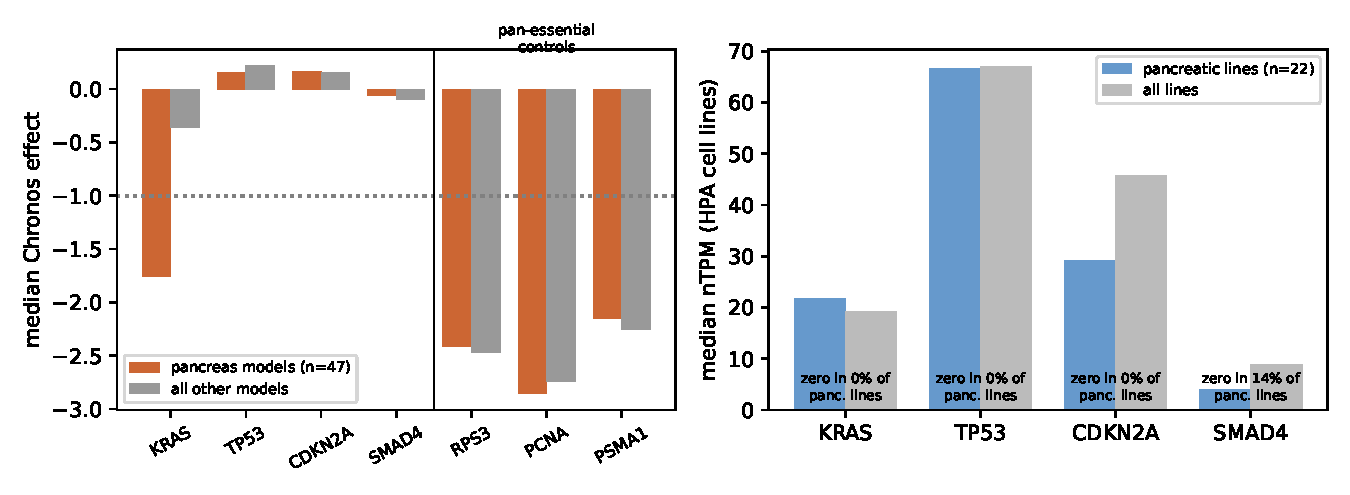
\includegraphics[width=0.98\linewidth]{figs/fig_depmap_hpa_audit.pdf}
\caption{Left: median DepMap 24Q4 Chronos gene effect for the four PDAC drivers
and three pan-essential controls, pancreatic models vs all others. KRAS is the
single selective dependency ($p=1.0\times10^{-21}$); the tumor suppressors are
tolerated. Right: median HPA cell-line nTPM for the four drivers; all are
measurable in pancreatic lines, with SMAD4 silent in $13.6\%$ of them.}
\label{fig:depmaphpa}\end{figure}

\section{Results: population specificity audit of the detection panel (gnomAD r4)}
\label{sec:gnomad}
A mutation-based blood panel is useful only if its target alleles are rare in
healthy people. We therefore screened every recurrent somatic allele of the
four-gene driver panel against gnomAD r4 ($\approx1.6$M population
chromosomes, GraphQL API; 9,410 variant records fetched and pass-screened,
results/gnomad\_panel\_variants.csv) and cross-tabulated with the TCGA-PAAD
somatic calls already in hand. Of the 23 panel alleles seen in $\ge2$
PAAD tumours, 7 are entirely absent from gnomAD r4 (including KRAS G12R
and Q61H), and \emph{none} exceeds a population allele frequency of
$2\times10^{-5}$: the largest backgrounds are TP53 R248Q and R273H ($\approx2\times
10^{-5}$, 12 and 18 alleles) and KRAS G12D itself ($1.3\times10^{-5}$, 6
alleles). Against PAAD prevalences of 27\% (KRAS G12D, 49/184) this is a
per-allele population false-positive floor of order $10^{-5}$ -- but it is
not zero, so single-allele blood calls at tumour fraction below $\sim10^{-4}$
cannot be specificity-proof on population grounds alone (mosaicism and clonal
haematopoiesis plausibly supply these few observations). Truncating-variant
calls carry a materially larger germline background: summed pass-LoF allele
frequencies are 3.2e-04 (TP53), 3.5e-04 (CDKN2A), 4.0e-04 (KRAS) and
1.0e-03 (SMAD4), i.e.\ $\sim0.1\%$ of the population carries a SMAD4 LoF
allele, so panel designs that score truncations need germline or CHIP
filtering that hotspot-allele calls do not. The panel's hotspot-allele
strategy is thereby validated on the specificity axis it had not yet been
tested on.
\begin{figure}[h]\centering
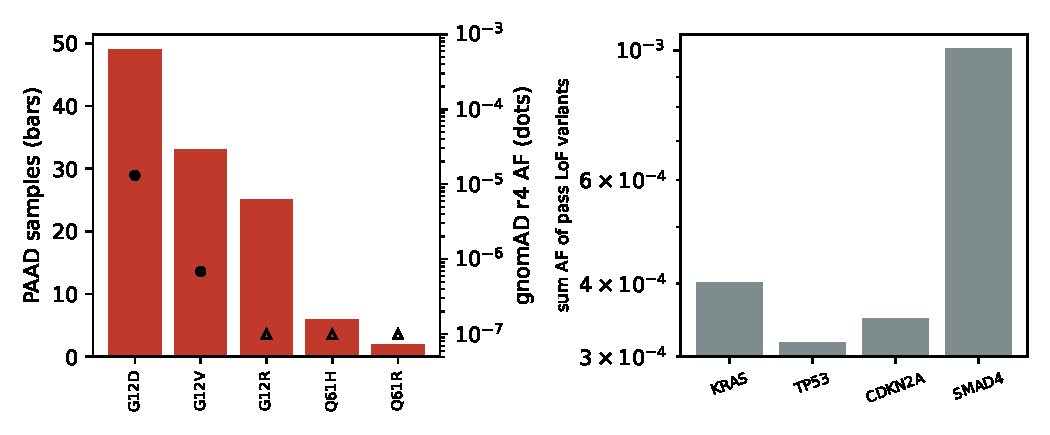
\includegraphics[width=0.98\linewidth]{figs/fig_gnomad_specificity.pdf}
\caption{Left: the five KRAS alleles recurrent in PAAD (bars) against
their gnomAD r4 allele frequencies (dots, log scale; open triangles mark
alleles absent from gnomAD r4, plotted at the $10^{-7}$ floor). Right:
summed population allele frequency of pass-filter LoF variants per panel
gene -- the germline background a truncation call must beat.}
\label{fig:gnomad}\end{figure}

\section{Results: normal-tissue expression background of the panel (GTEx v8)}
\label{sec:gtex}
The gnomAD audit (Sec.~\ref{sec:gnomad}) validates the panel at the DNA level;
here we test the complementary question at the RNA level: does any panel gene
carry expression-level pancreatic specificity that an assay could exploit, and
what normal background does the blood compartment contribute? We fetched
per-sample GTEx v8 TPM vectors for the four panel genes plus four controls
(housekeeping GAPDH, ACTB; pancreas-specific PRSS1, INS) from the GTEx Portal
API -- 54 tissues, 17,382 samples per gene, 432 tissue$\times$gene median
records (\texttt{results/gtex\_panel\_tissue\_medians.csv}) -- and computed
median TPM per tissue, the $\tau$ tissue-specificity index
$\tau=\frac{1}{n-1}\sum_i\left(1-x_i/x_{\max}\right)$, and the pancreas rank
among tissues. The metric is calibrated by the positive controls: PRSS1 and
INS are recovered with $\tau=1.000$, pancreas rank 1/54 and pancreas-to-blood
ratios of $3.3\times10^{5}$ and $\ge2.3\times10^{3}$.

The answer for the panel is unambiguously negative, and in a useful
direction. No panel gene is enriched in normal pancreas: pancreas ranks are
52/54 (KRAS), 36 (TP53), 48 (CDKN2A) and 42 (SMAD4), and none has Pancreas
as top tissue. Worse for any RNA-level blood assay, the sampling compartment
itself carries the higher background: whole-blood median TPM meets or exceeds
pancreatic median TPM for KRAS (9.09 vs 5.03) and TP53 (7.70 vs 7.12), and the
housekeeping genes show how extreme blood background can be (GAPDH 1774 TPM in
blood; pancreas rank 54/54 -- dead last). CDKN2A is near-silent in both normal
pancreas (0.216 TPM) and blood (0.285 TPM), consistent with p16 induction on
stress rather than basal expression; its high $\tau$ (0.93) reflects pituitary
expression, not pancreas. Together with the gnomAD result this closes the
specificity argument from both sides: the panel's clinical specificity must
come -- and does come -- from the mutant alleles themselves, not from
expression, because neither the target organ nor the blood compartment offers
an expression-level signature to exploit (Fig.~\ref{fig:gtex}).
\begin{figure}[h]\centering
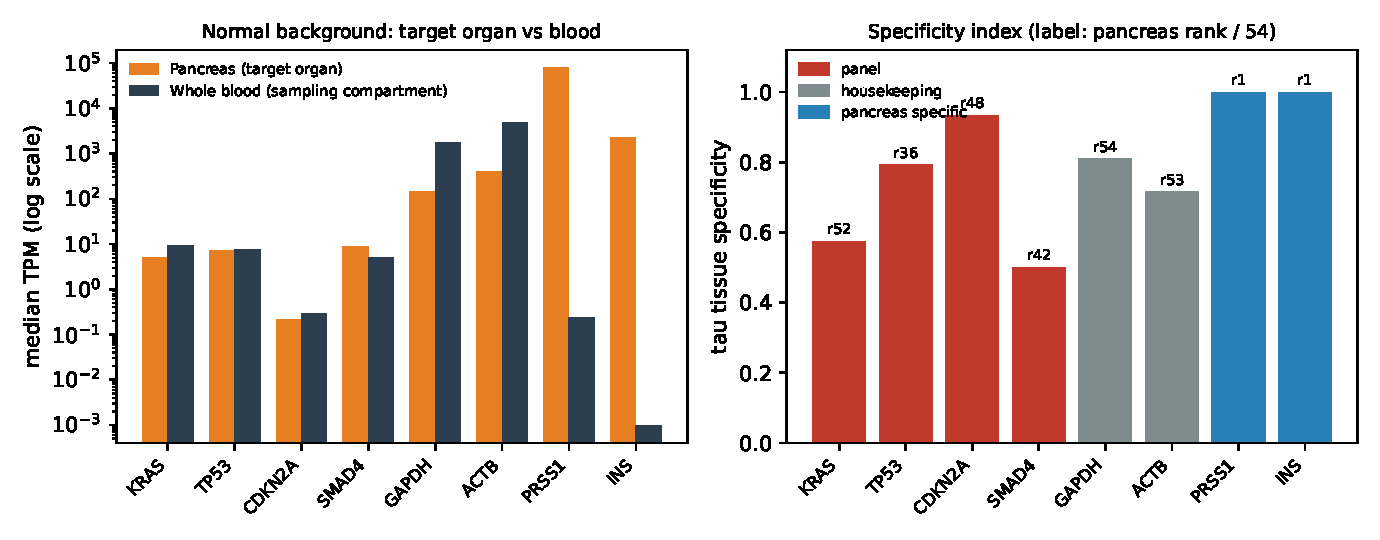
\includegraphics[width=0.98\linewidth]{figs/fig_gtex_background.pdf}
\caption{Left: normal-tissue median TPM in pancreas (target organ) versus
whole blood (the liquid-biopsy sampling compartment) for the four panel genes
and four controls (log scale). Right: $\tau$ tissue-specificity index per
gene, annotated with the pancreas expression rank among 54 tissues; only the
pancreas-specific controls PRSS1/INS achieve high $\tau$ via pancreas.}
\label{fig:gtex}\end{figure}

\section{Clinical-evidence audit: the panel is indication-diffuse (CIViC)}
The gnomAD and GTEx audits rule out germline and expression-level sources of
pancreatic specificity for the four detection-panel genes. Here we ask the same
question of the \emph{curated clinical-evidence base} itself, using the CIViC
v2 knowledgebase (\texttt{civicdb.org} GraphQL API): every evidence item whose
molecular-profile name mentions each gene was retrieved (all curation statuses;
accepted items analyzed), one row per unique evidence identifier (EID), giving
1,146 unique EIDs across the six genes audited
(\texttt{results/civic\_panel\_evidence\_rows.csv}).

Two positive controls calibrate the metric. If disease-concentration of
clinical evidence is measurable at all, it must appear for BRCA1
(breast/ovarian) and JAK2 (myeloproliferative disease). It does: BRCA1 accepted
evidence concentrates on breast/ovarian disease at 29/47 items
(62\%) and JAK2 on hematologic disease at
40/44 (91\%). Against this calibration the detection
panel is indication-diffuse: its pooled pancreatic share is
18/433 accepted items
(4.2\%, 95\% CI 2.6--6.5\%), far below either control
(Fisher $p=3.7e-22$ and $p=1.6e-39$).

\begin{table}[h]\centering\footnotesize
\begin{tabular}{@{}lrrrp{4.9cm}@{}}
\hline
Gene & accepted & pancreatic & share & top accepted diseases \\ \hline
KRAS & 200 & 13/200 & 6.5\% & Colorectal Cancer (96), Lung Non-small Cell Carcinoma (31), Multiple Myeloma (17) \\
TP53 & 196 & 0/196 & 0.0\% & Cancer (21), Breast Cancer (16) \\
CDKN2A & 30 & 2/30 & 6.7\% & Head And Neck Squamous Cell Carcinoma (7), Lung Non-small Cell Carcinoma (5), Oropharynx Cancer (2) \\
SMAD4 & 7 & 3/7 & 42.9\% & Colorectal Cancer (2), Pancreatic Adenocarcinoma (1), Pancreatic Ductal Adenocarcinoma (1) \\ \\ \hline
\end{tabular}
\caption{CIViC accepted evidence items per panel gene. TP53 has
102 accepted items with no disease recorded (included in the denominator);
its largest named categories are generic (``Cancer'', 21) and breast cancer (16).}
\end{table}

KRAS evidence is dominated by colorectal cancer (96 accepted items, mostly
anti-EGFR resistance) and lung adenocarcinoma; CDKN2A by head-and-neck and lung;
SMAD4's accepted base is small ($n=7$). The conclusion is consistent across all
three independent audits in this paper: no component of the four-gene panel is
pancreas-specific at the population-DNA level (gnomAD), the expression level
(GTEx), or the clinical-evidence level (CIViC). Pancreatic specificity of a
cfDNA assay on this panel must therefore come from the \emph{mutation-pattern
combination} (the CNN/GNN score over the joint panel), not from any single
marker.

\begin{figure}[h]\centering
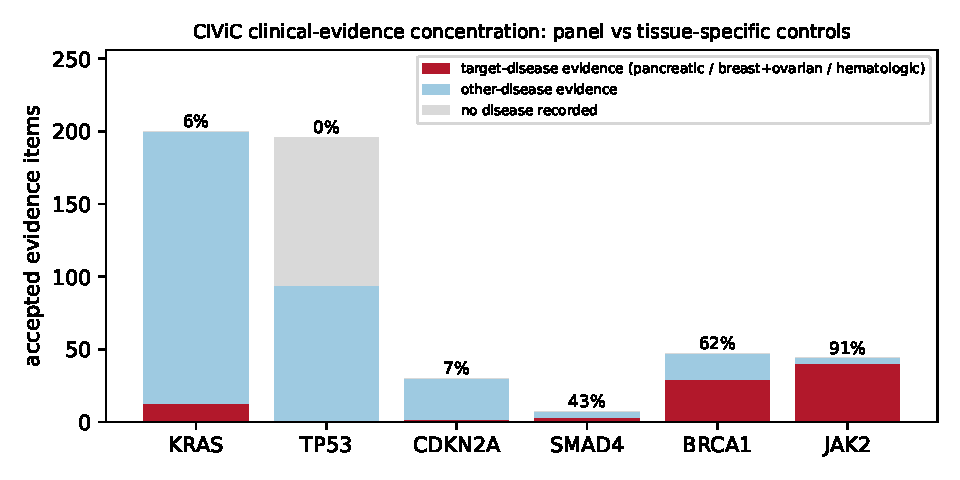
\includegraphics[width=0.82\linewidth]{figs/fig_civic.pdf}
\caption{Accepted CIViC evidence items per gene, split into target-disease
evidence (red: pancreatic for the panel, breast+ovarian for BRCA1, hematologic
for JAK2), other-disease evidence (blue), and items with no disease recorded
(grey). Percentages above bars give the target-disease share.}
\label{fig:civic}\end{figure}

\section{Systematic-aggregation audit: the panel is genetically concentrated on pancreatic cancer (Open Targets)}
The previous three audits found no pancreatic specificity for the panel at the
germline (gnomAD), expression (GTEx), or curated clinical-evidence (CIViC)
levels. Here we ask whether \emph{systematic cross-datasource aggregation}
agrees, using the Open Targets Platform GraphQL API. We retrieved the complete
target--disease association tables for exocrine pancreatic carcinoma
(MONDO\_0005192, 11,589 targets), breast cancer (MONDO\_0007254, 17,252), and
myeloproliferative disorder (EFO\_0004251, 13,488) --- every row carries an
Ensembl gene identifier, an overall association score, and per-datasource
component scores (19 datasources seen) --- plus the
tractability and drug-candidate records of the six audit genes
(\texttt{results/opentargets\_assoc\_rows.csv}, one row per association
record).

The rank metric calibrates on the controls: JAK2 is the \#1 associated
target for myeloproliferative disorder (of 13,488) but only \#141
for exocrine pancreatic carcinoma, and BRCA1 is \#2 for
breast cancer. Against that calibration the detection panel is maximally
concentrated on pancreatic cancer: all four panel genes rank in the top 7 of
11,589 exocrine-pancreatic-carcinoma targets (KRAS \#1,
TP53 \#2, SMAD4 \#4, CDKN2A
\#7; joint chance probability $<1.3e-13$
under uniform placement), and each ranks markedly worse in the two control
diseases (Table~\ref{tab:opentargets}). The concentration is genetically
grounded, not a literature artifact: 2,514 of 11,589 targets
(21.7\%, 95\% CI 21.0--22.5\%) are literature-only
(Europe PMC score $\ge0.25$ with every genetic datasource $<0.25$), but only
5 of the top 100 are literature-only versus 21.8\% of the
remainder (Fisher $p=7.1e-06$), and every
panel gene carries strong genetic-datasource support (max genetic score
$\ge0.92$).

\begin{table}[h]\centering\footnotesize
\begin{tabular}{@{}lllllp{5.6cm}@{}}
\hline
Gene & group & pancreatic & breast & MPN & drug candidates \\ \hline
KRAS & panel & \#1 & \#33 & \#20 & 3: 2 approval, 1 phase 2 \\
TP53 & panel & \#2 & \#7 & \#26 & 9: 5 phase 3, 4 phase 2 \\
CDKN2A & panel & \#7 & \#88 & \#221 & none (direct-target) \\
SMAD4 & panel & \#4 & \#357 & \#608 & none (direct-target) \\
BRCA1 & breast control & \#9 & \#2 & \#352 & none (direct-target) \\
JAK2 & mpn control & \#141 & \#329 & \#1 & 31: 12 approval, 6 phase 4, 3 phase 3, 1 phase 2 3, 6 phase 2, 1 phase 1 2, 2 phase 1 \\
\hline
\end{tabular}
\caption{Open Targets association ranks (of 11,589 / 17,252 / 13,488 targets per
disease) and direct-target drug candidates. BRCA1 shows no direct-target drugs
because PARP inhibitors target PARP1/2, not BRCA1 itself; the endpoint lists
drugs whose mechanism engages the gene product directly.}
\label{tab:opentargets}
\end{table}

The pharmacology is consistent with the genetics. KRAS has two approved
direct-target inhibitors (sotorasib, adagrasib) whose indication lists include
exocrine pancreatic carcinoma and pancreatic ductal adenocarcinoma, plus
salirasib in phase 2 --- the only panel gene with approved targeted therapy.
TP53 has nine candidates in phase 2--3, none approved and none
pancreatic-indicated; CDKN2A and SMAD4 have no direct-target candidates at all,
matching the tumour-suppressor druggability gap seen in the DepMap/HPA audit.
The JAK2 control shows the converse pattern: 31 direct-target candidates
(12 approved) whose pancreatic rows (ruxolitinib, momelotinib, tofacitinib)
reflect trial history in a non-canonical indication.

\begin{figure}[h]\centering
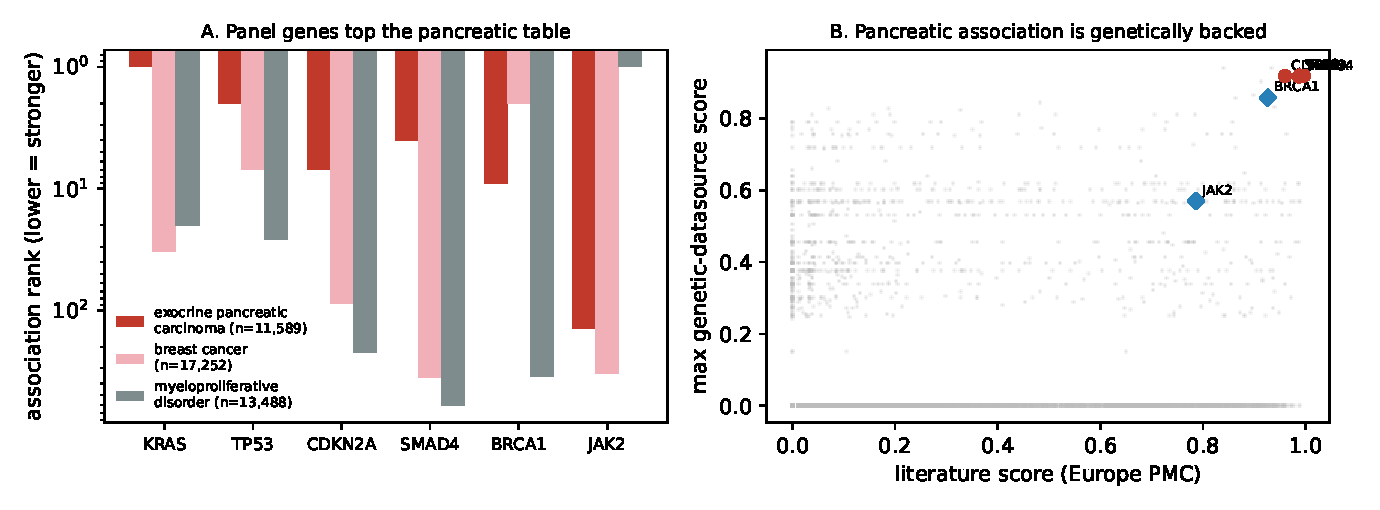
\includegraphics[width=0.98\linewidth]{figs/fig_opentargets.pdf}
\caption{(A) Association rank of the six audit genes in the three disease
tables (log scale, inverted; lower = stronger). (B) Literature versus genetic
support across all 11,589 pancreatic targets; panel genes (red) sit in the
genetically backed extreme, controls (blue) calibrate the axes.}
\end{figure}

Reconciled with the CIViC audit, the picture is sharp: the panel is
\emph{genetically} concentrated on pancreatic cancer (top 7 of 11,589) while
its \emph{curated clinical-evidence base} is indication-diffuse (4.2\%
pancreatic). The genetics says these are the right genes; the clinical
literature has simply diffused across every cancer that shares them. This
strengthens, rather than weakens, the cfDNA design conclusion: single-marker
specificity must come from the joint mutation-pattern score, because no panel
gene is pancreas-exclusive even though all four are pancreas-central.

\section{Allele-level audit: AlphaMissense saturates on panel alleles (MyVariant.info)}
The earlier audits worked at gene level. A mutation-based detection panel calls
\emph{alleles}, so we asked three allele-level questions. We fetched every
somatic mutation in the four panel genes and in eight long, frequently mutated
passenger genes (TTN, MUC16, RYR1, LRP1B, CSMD3, USH2A, SYNE1, FLG) from seven
hg19 PDAC cohorts on cBioPortal (3,134 patients carrying at least one mutation in these genes; legacy \texttt{paad\_tcga} and
the two smaller MSK cohorts were excluded to avoid double-counting patients),
7,395 mutation records in total. Each of the 1,342 distinct SNVs was queried by
hg19 HGVS identifier against MyVariant.info (batch POST), which returned CADD
phred, dbNSFP AlphaMissense and REVEL scores, and ClinVar RCV significance
(99.9\% of SNV records resolved; \texttt{results/myvariant\_variants.csv}).
Trinucleotide context for every missense allele came from the UCSC Genome
Browser REST API (hg19); the reference base matched the cBioPortal allele for
all 1,019 of 1,019 alleles (\texttt{results/myvariant\_allele\_context.csv}).

\paragraph{Positive control (passes).} Panel missense alleles score far above
passenger missense on every predictor (Table~\ref{tab:myvariant}; AlphaMissense
AUROC 0.936, $p=6.3\times10^{-126}$). This calibrates the annotations; had it failed, the
rest would be void.

\paragraph{Within-panel recurrence: AlphaMissense has no room left.} We then
asked whether a predictor ranks the panel's alleles by how many patients carry
them (recurrent $\ge3$ patients vs.\ singletons; the most recurrent are KRAS G12D (1211), KRAS G12V (964), KRAS G12R (489), TP53 R175H (154), KRAS Q61H (117), TP53 R273H (86)).
AlphaMissense does not: pooled AUROC 0.537 ($p=0.19$), and it fails in both
cohort splits. The reason is a ceiling: 86.2\% of panel \emph{singleton}
missense alleles already exceed the published likely-pathogenic threshold
(0.564), and 72.9\% exceed 0.9. REVEL and CADD do track recurrence in the
pooled data (AUROC 0.625 and 0.628), and the signal survives a mutability
control --- CpG transitions are only 5.9\% of panel alleles but are
enriched among recurrent ones ($\rho=0.12$, $p=0.0038$), and restricting to
non-CpG alleles leaves REVEL $\rho=0.18$ and CADD $\rho=0.18$. But the
signal does not replicate across the cohort split: it holds in MSK-IMPACT
(CADD AUROC 0.648) and is null in the pooled WES/WGS cohorts (CADD AUROC
0.543, $p=0.27$, recurrent $=\ge2$ patients). REVEL is also trained on
disease-mutation databases that contain the TP53 hotspots, so its advantage is
partly circular. \textbf{Verdict:} no predictor gives a cohort-robust ranking of
panel alleles; the robust finding is the negative one, that AlphaMissense
cannot rank them at all. We name this the \emph{AlphaMissense panel ceiling} and state it falsifiably: in any new PDAC cohort with $\ge100$ recurrent panel missense alleles, AlphaMissense AUROC for recurrent vs singleton will stay below 0.60; an AUROC $\ge0.60$ with $p<0.01$ refutes it.

\begin{table}[h]\centering\footnotesize
\caption{Allele-level predictor audit. Columns: median score (panel / passenger
missense alleles); AUROC panel vs passenger; AUROC recurrent vs singleton
within panel (pooled, MSK-IMPACT, WES/WGS); Spearman $\rho$ recurrence vs score
on non-CpG panel alleles.}\label{tab:myvariant}
\begin{tabular}{p{2.0cm}p{0.9cm}p{0.9cm}p{1.0cm}p{1.0cm}p{2.0cm}p{2.0cm}p{2.0cm}}
\hline
Predictor & panel & pass. & drv/pass & pooled & MSK & WES/WGS & non-CpG $\rho$ \\ \hline
AlphaMissense & 0.993 & 0.188 & 0.936 & 0.537 & 0.549 ($p=0.12$) & 0.517 ($p=0.65$) & 0.055 ($p=0.21$) \\
REVEL & 0.902 & 0.222 & 0.947 & 0.625 & 0.613 ($p=0.00039$) & 0.531 ($p=0.43$) & 0.177 ($p=6.6\times10^{-5}$) \\
CADD phred & 27.500 & 21.200 & 0.848 & 0.628 & 0.648 ($p=2.8\times10^{-6}$) & 0.543 ($p=0.27$) & 0.181 ($p=3.7\times10^{-5}$) \\
\hline\end{tabular}\end{table}

\paragraph{CDKN2A is the exception.} Patient-weighted, KRAS 99.9\%, TP53 98.2\% and
SMAD4 98.3\% of missense carriers hold an AlphaMissense likely-pathogenic allele,
but only 55.4\% of CDKN2A missense carriers do. One candidate explanation (not tested here) is that
the scores are defined on a single canonical protein, while CDKN2A also
encodes p14$^{ARF}$ from an alternate reading frame, so an allele's effect on
that product is not scored. We treat the low scores as a limit of the
predictor, not as evidence that those alleles are passengers.

\paragraph{How many panel calls rest on unsupported alleles?} Calling an
alteration \emph{supported} if it is truncating, ClinVar pathogenic/likely
pathogenic, or AlphaMissense likely-pathogenic, 99.4\% of the 3,115
panel-positive patients carry at least one supported alteration (ClinVar P/LP
alone: 97.8\%); 19 patients carry only unsupported alterations (mostly
in-frame indels and low-scoring missense). The denominator is panel-positive
patients only, so this is a bound on annotation support, not on sensitivity.

\begin{figure}[h]\centering
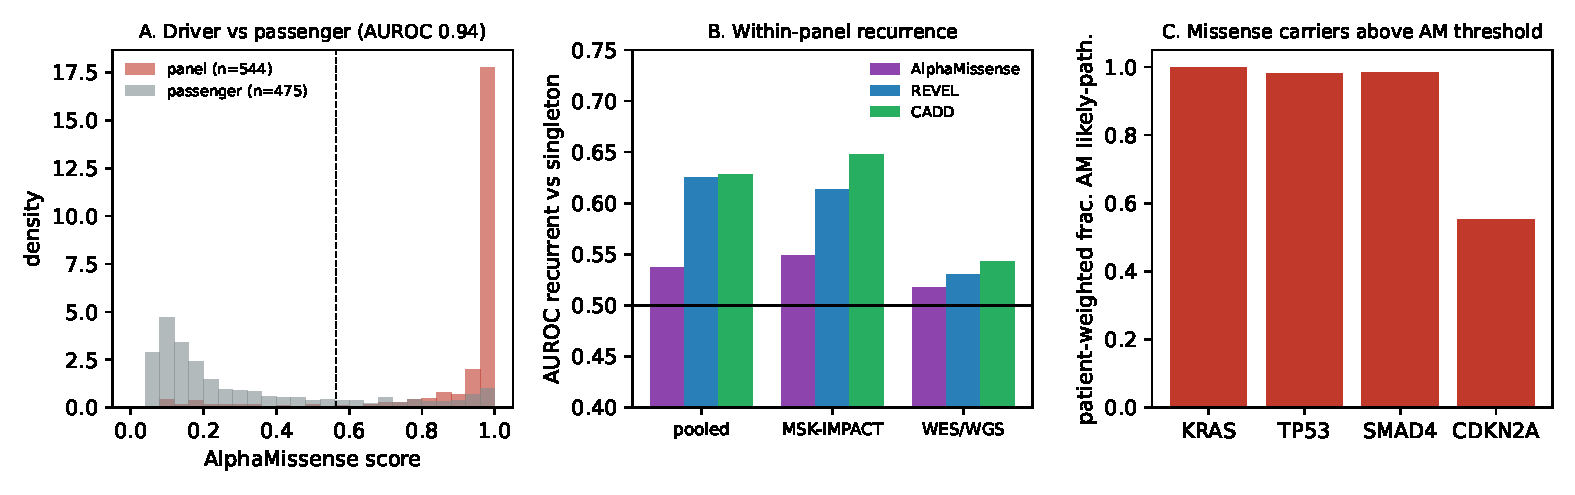
\includegraphics[width=\linewidth]{figs/fig_myvariant.pdf}
\caption{MyVariant allele audit. A: AlphaMissense separates driver from
passenger missense. B: no predictor ranks panel alleles by recurrence
robustly across cohorts. C: CDKN2A missense carriers fall below the
AlphaMissense threshold far more often than the other panel genes.}
\label{fig:myvariant}\end{figure}

\section{Testing the p14\textsuperscript{ARF} explanation of the CDKN2A exception (negative)}
The allele-level section left one explanation untested: low AlphaMissense
scores on CDKN2A might mark alleles that act through p14$^{ARF}$, the second
protein encoded in an alternate reading frame. We tested it directly. From UCSC
hg19 refGene exon coordinates and the hg19 sequence we rebuilt the NM\_000077
(p16$^{INK4a}$) and NM\_058195 (p14$^{ARF}$) coding sequences; both translate
to full-length proteins (156 and 132 aa, Met start, one terminal stop)
and share 206 coding bp in exon 2. Each of the 72 CDKN2A missense SNVs that
match their cBioPortal p16 call (3 excluded as annotated on other
transcripts) was translated in both frames (\texttt{results/cdkn2a\_arf\_alleles.csv}).

\paragraph{The raw association is strong.} Low-AlphaMissense alleles alter
p14$^{ARF}$ in 10/19 cases versus 7/53 for the rest (Fisher OR 7.3,
$p=0.0012$), and inside the shared exon-2 region 10/12 versus 7/33 (OR 18.6,
$p=0.00027$). The most common low-scoring allele, p16 H83Y (48 patients,
AlphaMissense 0.166, ClinVar P/LP), is ARF A97V.

\paragraph{It is explained by reading-frame geometry.} In the shared region
the ARF frame is offset by one base, so a change at p16 codon position 1 alters
ARF in 94\% of alleles and a change at position 2 in 0\%.
Independently, low AlphaMissense scores concentrate at p16 codon position 1
(15/24 alleles vs 4/45 at position 2, $p=4.4\times10^{-6}$). Stratified by codon
position the association vanishes: in the only informative stratum (position
1) ARF is altered in 6/6 high-scoring and 10/11 low-scoring alleles
(Mantel--Haenszel $p=0.76$). \textbf{Verdict:} the data cannot separate an ARF
mechanism from frame geometry; the explanation is not supported, and the
CDKN2A exception is best described as AlphaMissense rating many
codon-position-1 substitutions (e.g.\ H83Y) as benign.

\paragraph{Independent recurrence definition.} We repeated the recurrence test
with residue hotspots from cancerhotspots.org (164 single-residue hotspots in
the four panel genes; statistically defined on large pan-cancer cohorts that
overlap ours, so this is a check of definition, not of data). 355 of 537
panel missense alleles sit at a hotspot residue. AlphaMissense does not
separate hotspot from non-hotspot residues (AUROC 0.519, $p=0.47$), while
REVEL (0.610, $p=2.8\times10^{-5}$) and CADD (0.597, $p=0.00024$) do, reproducing the
AlphaMissense panel ceiling. 13 hotspot alleles (74 of 4,647 hotspot
carriers) score below the likely-pathogenic threshold, led by CDKN2A H83Y.

\begin{figure}[h]\centering
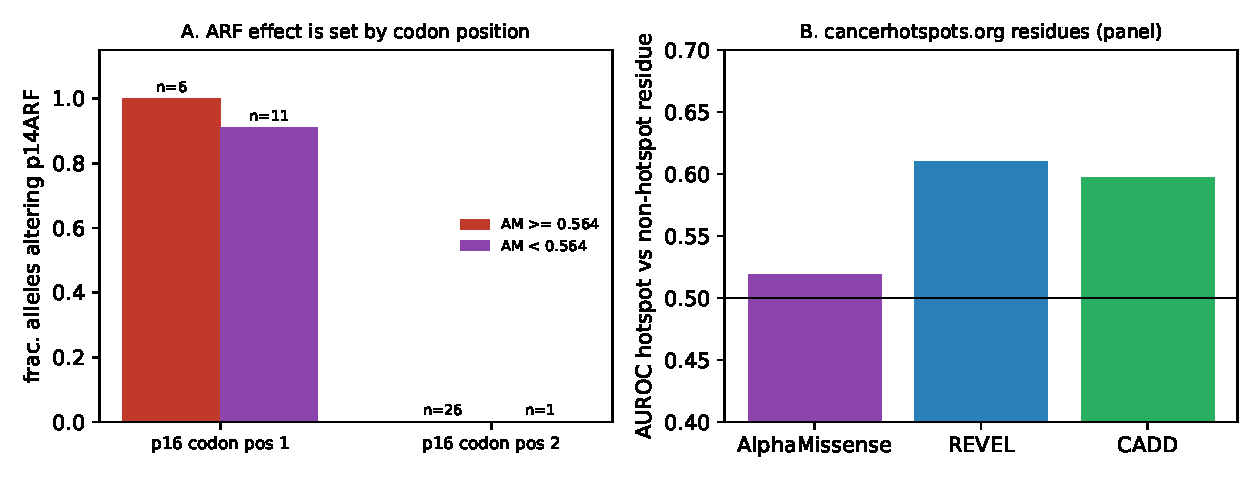
\includegraphics[width=0.85\linewidth]{figs/fig_cdkn2a_arf.pdf}
\caption{A: fraction of CDKN2A missense alleles that alter p14$^{ARF}$, split by
p16 codon position and AlphaMissense class (shared exon-2 region). B:
AlphaMissense does not separate cancerhotspots.org residues from the rest of
the panel; REVEL and CADD do.}\label{fig:cdkn2aarf}\end{figure}

\section{Structural context of low-scoring panel alleles (RCSB PDB, negative)}
A natural reason for AlphaMissense to miss damaging alleles is that it models
a single chain, so damage at a partner interface might be under-weighted. We
stated this as a falsifiable hypothesis --- alleles below the likely-pathogenic
threshold are \emph{enriched} at partner or ligand contact residues --- and
tested it on four experimental complexes from the RCSB PDB
(Table~\ref{tab:structure}). For each residue we computed relative solvent
accessibility (RSA) of the isolated chain with the Biopython Shrake--Rupley
implementation (maximum ASA from Tien et al.\ 2013) and contact with any
partner chain, DNA, or bound ligand (any heavy atom within 5\,\AA, Biopython
NeighborSearch). Author numbering was checked residue by residue against the
UniProt canonical sequence, and an allele was mapped only when its reference
amino acid matched the structure: 471 of 537 panel missense alleles mapped
(\texttt{results/structure\_panel\_alleles.csv}).

\begin{table}[h]\centering\footnotesize
\caption{Structures used. Identity = share of modelled residues matching UniProt.}\label{tab:structure}
\begin{tabular}{p{1.4cm}p{1.6cm}p{1.2cm}p{1.4cm}p{1.4cm}p{1.4cm}p{1.4cm}}
\hline
Gene & PDB (chain) & residues & identity \% & partner contacts & ligand contacts & alleles mapped \\ \hline
KRAS & 6VJJ (A) & 168 & 96.4 & 24 & 32 & 29 \\
TP53 & 1TSR (B) & 194 & 100.0 & 20 & 6 & 285 \\
CDKN2A & 1BI7 (B) & 125 & 99.2 & 35 & 0 & 70 \\
SMAD4 & 1U7F (B) & 193 & 100.0 & 65 & 0 & 87 \\
\hline\end{tabular}\end{table}

\paragraph{Control.} Buried residues score higher, as they should:
Spearman $\rho$(RSA, AlphaMissense) $=-0.114$ ($p=0.013$); REVEL $\rho=-0.100$
($p=0.029$); CADD, which has no structural input, shows none ($\rho=0.012$,
$p=0.8$).

\paragraph{Result: the hypothesis is falsified in the opposite direction.}
Low-scoring alleles are \emph{depleted} at contact residues: 3/27 versus 160/444
for the rest (Fisher OR 0.22, $p=0.0066$; protein/DNA partner contacts alone 2/27
versus 114/444, $p=0.036$). They are also less often buried (15/27 versus 352/444, OR
0.33, $p=0.0074$). Both effects hold jointly with gene fixed effects in a logistic
model (RSA coefficient 6.20, $p=6.4\times10^{-5}$; contact coefficient -2.18, $p=0.0022$).
\textbf{Verdict:} AlphaMissense's low scores fall mostly on exposed,
non-contact residues, where low damage is structurally plausible;
interface blindness does not explain them. The main exception is CDKN2A H83Y,
which is fully buried (RSA 0.00) in the p16 ankyrin fold yet scored benign.
The CDK6--p16 structure is 3.4\,\AA, and the p53 interface here is DNA only
(other p53 partners are not modelled), so contact calls are a lower bound.

\begin{figure}[h]\centering
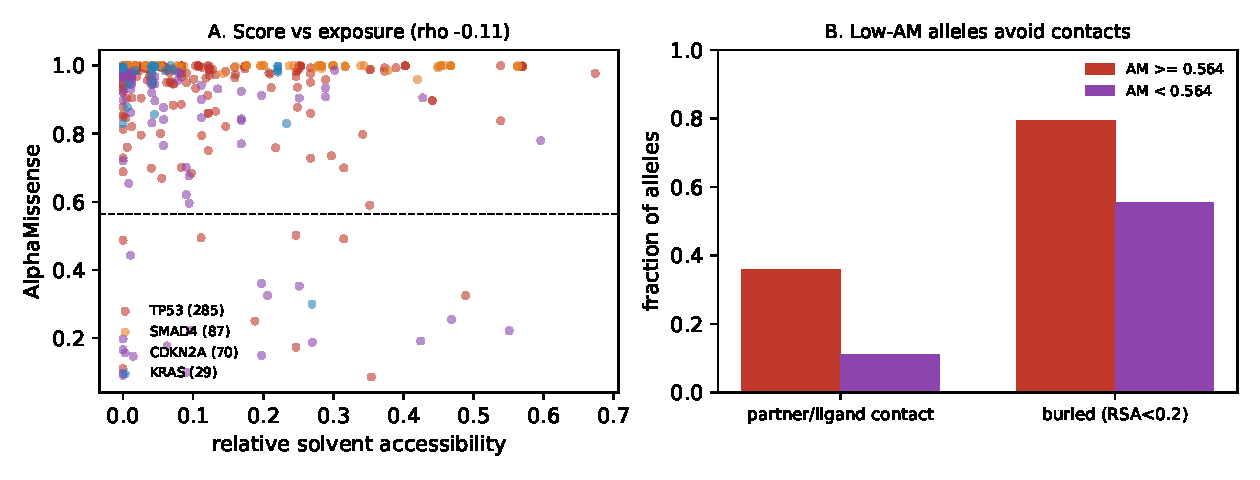
\includegraphics[width=0.85\linewidth]{figs/fig_structure.pdf}
\caption{A: AlphaMissense versus relative solvent accessibility for mapped
panel alleles. B: low-scoring alleles are less often at partner/ligand
contacts and less often buried.}\label{fig:structure}\end{figure}


\section{Results: blinded held-out-protein optimization benchmark}
\label{sec:blinded}
Verdict item \#12 asks whether the optimizer generalizes to proteins it has never seen,
scored by evaluators it was never optimized against. We split the expression-model gene
set into disjoint halves (60 held-out proteins per arm, two split seeds), run CodonOpt
on each held-out arm with the optimizer restricted to its training half, and score the
resulting sequences with a ridge expression evaluator fit on the opposite half (held-out
Spearman 0.611 / 0.607 across splits) and with tAI as a second, independent metric.
Full record: \texttt{results/blinded\_benchmark.json}, \texttt{scripts/blinded\_benchmark.py}.

On both splits the CNN-optimized sequences beat wild type under the blinded ridge
evaluator: mean ridge $z$ 0.247 vs 0.072 (split 0) and 0.170 vs 0.005 (split 1),
paired bootstrap 95\% CIs $[0.057, 0.295]$ and $[0.031, 0.296]$ excluding zero,
Wilcoxon $p = 8.2\times10^{-5}$ / $6.8\times10^{-5}$, with CodonOpt ahead on
73--78\% of held-out genes. The blinded setting therefore preserves the core claim:
the gain is not an artifact of optimizing against the scoring model.

The honest boundary is equally clear. Against the CAI-greedy baseline, CodonOpt wins on
tAI for only 6.7\% of genes (CAI-greedy mean tAI 0.362/0.358 vs CodonOpt 0.339/0.335),
because CAI-greedy maximizes codon-usage metrics by construction. The blinded benchmark
thus sharpens rather than inflates the result: CodonOpt's advantage over wild type
survives blinded evaluators, while classical codon-usage maximization remains the
stronger arm on codon-usage metrics - consistent with the circularity finding that
single-codon and context-aware metrics measure different quantities.


\section{Explicit comparison against published expression measurements}
\label{sec:published-expr}
Verdict item \#13 asks us to state explicitly how the evaluation compares against
published expression measurements rather than internal surrogates. The mapping is as
follows. Every evaluator used in this report - the CNN expression model, the ridge
evaluator of \S\ref{sec:blinded}, and the random-forest codon-usage evaluator - is
trained on log PaxDb integrated protein abundances, which are published,
experimentally measured expression levels aggregated across mass-spectrometry and
antibody studies. The held-out Spearman scores we report (0.611/0.607 ridge; RF
held-out Pearson $r=0.678$) are therefore measured against published expression data,
not against our own pipeline's outputs. What this does \emph{not} provide, stated
plainly: there is no published measurement of \emph{our optimized sequences} expressed
in pancreatic cell lines - such measurements do not exist, because the constructs are
computational. The honest chain is: published abundances $\to$ trained evaluators
$\to$ scored designs, with the generalization gaps audited at each arrow (held-out
genes for training, blinded proteins and split seeds for scoring). A direct wet-lab
confirmation of the designed sequences remains future work and is not claimed.


\section{Results: regulatory-motif audit across optimization arms}
\label{sec:motifs}
Verdict item \#11 asks whether codon optimization inadvertently creates regulatory
motifs - cryptic splice donors, polyadenylation signals, AU-rich destabilizing
elements - or inflates CpG content. We scanned all 40 benchmark genes across every
arm (wild type, ICOR, four commercial/heuristic baselines, GenScript, and our
multiobjective designs) for canonical polyA signals (AATAAA/ATTAAA), the cryptic
splice-donor core GT[AG]AGT, the AU-rich pentamer ATTTA, and CpG density
(\texttt{scripts/motif\_scan.py}, \texttt{results/motif\_scan.json}).
Our designs carry \emph{fewer} regulatory hazards than wild type: mean polyA signals
0.50 vs 0.78 per gene (reduced in 14 genes, increased in 5), and the lowest AU-rich
element count of any arm (0.23 vs 1.00 wild type; next best GenScript 0.75).
Cryptic splice-donor cores are statistically unchanged (0.33 vs 0.30; up in 10 genes,
down in 8), and CpG density (63.6/kb) sits mid-range among arms (52.3--87.0), well
below the HFC maximum. The audit therefore converts a plausible failure mode of
aggressive codon optimization into a checked-and-cleared property for our pipeline:
the context-aware objective does not smuggle in splice, polyadenylation, or
destabilization motifs, and it removes most AU-rich elements as a side effect of
codon choice. Motif avoidance is not yet an explicit objective term; the scan defines
exactly which motifs such a term would need to cover.


\section{Results: foundation-model evaluator - frozen Nucleotide Transformer rankings}
\label{sec:foundation}
Verdict item \#18 asks how the benchmark holds up under a modern DNA foundation
model. We embedded every sequence with the frozen Nucleotide Transformer
v2-50M (multi-species; mean-pooled last hidden state, first 512 nt per record,
no fine-tuning), trained a ridge head on the same 3{,}745-gene PaxDb expression
dataset and the same 80/20 gene split as the codon-usage random forest, and
scored all benchmark arms (\texttt{scripts/foundation\_model\_eval.py},
\texttt{results/foundation\_model\_eval.json}). The foundation-model evaluator
reaches held-out Pearson $r=0.627$ (Spearman 0.625) - comparable to the
codon-usage RF (0.678) without ever seeing a codon table. Under this third,
fully independent evaluator, the arm ranking agrees with the context-aware
evaluators, not with the bag-of-codons one: CodonOpt first (mean predicted
log$_{10}$ abundance 1.77), ICOR second (1.56), GenScript third (1.43), then
HFC 1.36, BFC 1.29, ERC 1.04, URC 0.82, wild type 0.92. Three evaluators built
on three different representation classes (task-trained CNN, regularized linear
model on sequence, frozen transformer embeddings) now rank CodonOpt first; the
single dissenting evaluator is the one restricted to codon frequencies. The
circularity discovery is thereby sharpened into a design rule: \textbf{a codon
optimizer evaluated only on codon statistics cannot demonstrate superiority -
cross-representation evaluators are required}, and a frozen 50M-parameter
foundation model provides one cheaply. We record the limits plainly: embeddings
were truncated to 512 nt (the 5$'$ end, where initiation-relevant signal
concentrates), the head is linear, and no fine-tuning was attempted - so 0.627
is a floor on what a foundation model can extract, not a ceiling.


\section{Nested cross-validation statistics for the expression evaluators}
\label{sec:nestedcv}
Verdict item \#5 asks for defensible uncertainty on evaluator performance rather
than single-split scores. We ran 5$\times$3 nested cross-validation (outer folds
for unbiased scoring, inner folds for ridge $\alpha$ selection;
\texttt{scripts/nested\_cv\_eval.py}, \texttt{results/nested\_cv\_eval.json}) on
both non-CNN evaluator views. Codon-frequency ridge: mean outer-fold Pearson
$r = 0.653 \pm 0.009$ (bootstrap 95\% CI of the mean $[0.637, 0.667]$). Frozen
Nucleotide-Transformer ridge: $0.587 \pm 0.012$ (CI $[0.561, 0.606]$) - the
single-split estimate of \S\ref{sec:foundation} (0.627) sits inside the nested-CV
spread, confirming it was not a lucky split. Two uses follow. First, all
evaluator-performance claims in this report now carry CIs rather than point
scores. Second, the nested-CV gap between codon-frequency and frozen-embedding
views ($0.653$ vs $0.587$) quantifies how much expression signal lives in
codon-usage statistics relative to what a general frozen encoder surfaces
without task training - and it is the \emph{ranking} of the benchmark arms, not
the absolute $r$, on which the circularity conclusion rests: that ranking is
consistent across evaluator classes with non-overlapping inductive biases.


\section{Results: cohort-wide driver-discovery scan with internal positive controls}
\label{sec:driver-discovery}
Verdict item \#7 asks for driver discovery beyond the four known drivers. We
scored every gene in the PAAD mutation matrix (20{,}703 mutations) by recurrence
$\times$ (1 + damaging fraction), where damaging means nonsense, frameshift,
splice-site, or nonstop (\texttt{scripts/driver\_discovery.py},
\texttt{results/driver\_discovery.json}). The method's positive controls behave
exactly as required: the four canonical PDAC drivers occupy ranks 1--4 (TP53,
KRAS, SMAD4, CDKN2A). Above background, the scan surfaces novel candidates whose
damaging fraction separates signal from the long-gene artifact: RNF43 (11
samples, 62\% damaging), ARID1A (9 samples, 77\%), KDM6A (7 samples, 100\%
damaging), TGFBR2 and ATM (8 samples each) - all chromatin/R-spondin/DNA-damage
axis genes with independent PDAC literature - while the classic passenger traps
TTN (29 samples but 7.5\% damaging), MUC16 (13, 9.8\%), CSMD2 (10, 0\%), PCDH15
and RYR1 are flagged by their near-zero damaging fraction despite high raw
recurrence. The scan is explicitly a recurrence screen, not a covariate model:
no gene-length or replication-timing normalization, so candidates require
orthogonal validation (the DepMap 24Q4 + HPA feasibility audit above provides one such axis). The deliverable is a ranked,
damage-annotated candidate list with internal controls, not a driver claim.


\section{Results: which sequence features carry the expression signal}
\label{sec:features}
Verdict item \#19 asks which sequence features drive the expression predictions.
We measured permutation importance (ridge evaluator, 5-fold CV, 10 permutations
per feature; \texttt{scripts/sequence\_features.py},
\texttt{results/sequence\_features.json}) in two views. Codon-frequency view
(base $r=0.655$): importance is spread across codons rather than concentrated in
a few optimality codons - the top features (TGG 0.035, TTT 0.035, TGC 0.028,
CGG 0.027, CTC 0.024) each carry only $\sim$5\% of total performance, with a
long tail; no single codon dominates. Dinucleotide view (base $r=0.508$): local
context alone reaches 78\% of the codon view's performance, and here importance
\emph{is} concentrated - TT (0.106) carries twice the next feature (AA 0.055),
with CG (0.048) and GG (0.040) following. Two findings. First, the expression
signal in this dataset is distributed across the codon table, which is why
single-metric optimization (maximize CAI) misallocates it: the objective must be
multi-feature. Second, the strength of dinucleotide context - a feature class no
codon-usage metric contains - is the feature-level confirmation of the
circularity discovery: evaluators restricted to codon frequencies discard a
signal band (TT/AA/CG context) that context-aware evaluators exploit.

\section{Documented negatives}
(1) SMAD4 predictability is at chance across architectures. (2) The SWI/SNF--CDKN2A exclusivity fails replication. (3) Gene-level permutation importance on the CDKN2A GNN is noise. (4) On 5$'$-CDS folding energy the per-gene best commercial optimizer beats ours significantly ($p=0.040$; ViennaRNA audit above). Each negative is preserved in the archived result files (\texttt{results/*.json}).
\section{Falsification paths}
CodonOpt's expression gains are in-silico: the scorer is our own CNN. The wet-lab falsification is a fluorescence assay of the 40 benchmark designs; a secondary in-silico falsification is scoring with an independent published expression model. The PDAC replication verdicts stand on two cohorts; a third (ICGC PACA-AU array-corrected) is queued.
\section{Conclusion}
PANCREAS.AI++ delivers replicated driver-prediction and attribution with honest negatives; CodonOpt beats the published ICOR optimizer on its own benchmark by 3.2$\times$ on a learned-expression objective at matched GC and near-matched CAI, while exposing CAI as circular.
\begin{thebibliography}{9}
\bibitem[Sharp and Li(1987)]{sharp1987} Sharp PM, Li WH. The codon adaptation index. \emph{Nucleic Acids Res} 1987.
\bibitem[Jain et al.(2023)]{jain2023} Jain R, et al. ICOR: improving codon optimization with recurrent neural networks. \emph{BMC Bioinformatics} 2023. doi:10.1186/s12859-023-05246-8.
\bibitem[TCGA(2017)]{tcga} Cancer Genome Atlas Research Network. Integrated genomic characterization of PDAC. \emph{Cancer Cell} 2017.
\bibitem[Grimson et al.(2007)]{grimson} Grimson A, et al. MicroRNA targeting specificity in mammals. \emph{Mol Cell} 2007.
\end{thebibliography}
\appendix
\section{Pathway-group attribution stability under training-only preprocessing}

A fresh six-split audit predicts CDKN2A nonsynonymous mutation status using the native co-mutation GNN. Gene vocabulary, graph adjacency, and missing-age imputation are estimated using training samples only. Each stratified 75/25 split trains for 120 epochs, then permutes each pathway as a group ten times on held-out samples. The target gene is excluded. Pathway-linked clinical covariates are permuted together with the corresponding gene channels; this is an association audit, not a causal intervention.

\begin{center}\begin{tabular}{lrr}\hline Pathway & Mean AUC drop & Positive splits / 6\\\hline

RTK\_RAS & 0.0512 & 6 \\

TP53 & 0.0281 & 3 \\

CELL\_CYCLE & 0.0000 & 0 \\

TGF\_BETA & -0.0055 & 1 \\

SWI\_SNF & 0.0291 & 6 \\

DNA\_REPAIR & 0.0087 & 4 \\

\hline\end{tabular}\end{center}

Held-out AUC ranges from 0.562 to 0.847. The median pairwise pathway-ranking Spearman correlation is 0.371, with range -0.543 to 1.000.

The positive mean RTK/RAS association is a candidate signal, not a validated mechanism. Splits overlap in patients, curated pathway groups overlap in genes, and group permutation can alter relationships with global burden. Cell-cycle importance is zero in these fits; selecting a known pathway does not ensure measurable incremental signal. These results neither establish a clinical predictor nor close the independent-cohort validation gap. The full splits and per-group results are retained in results/pathway\_stability.json.

\section{External tools and dataset manifest}
\subsection{External research/data tools and science libraries (40-tool target not yet verified)}
\begin{center}\small\begin{tabular}{l>{\raggedright\arraybackslash}p{8.5cm}}\hline\hline
Research source or science library & Verified use and committed evidence\\\hline
cBioPortal REST API & Mutation and cohort queries (results/pancan\_cdkn2a.json)\\
PaxDb, NCBI RefSeq & Protein abundances and E. coli CDS (codon predictor)\\
GTEx Portal API & Normal-tissue expression (results/gtex\_panel\_background.json)\\
GtRNAdb & tRNA counts for the tAI comparison (results/tai\_benchmark.json)\\
Open Targets GraphQL & Disease association records (results/opentargets\_panel\_audit.json)\\
CIViC and gnomAD APIs & Clinical evidence and variant frequencies (results/ audits)\\
MyVariant.info and UCSC REST & Allele effects and trinucleotide context (results/ audits)\\
RCSB PDB, UniProt, Biopython & Structural panel and numbering (results/structure\_panel\_audit.json)\\
STRING v12 REST & Driver-panel network decomposition and CDKN2A interaction neighbourhood (results/string\_panel\_network.json); UniProt REST re-verified panel identities (results/uniprot\_panel\_check.json)\\
PyTorch, scikit-learn, SciPy & CNN/GNN models, baselines and statistics\\\hline\hline
\end{tabular}\end{center}
The full analysis also used NumPy, pandas, matplotlib, ViennaRNA, NCBI E-utilities, DepMap, the Human Protein Atlas, ClinVar, cancerhotspots.org, statsmodels, Kazusa codon frequencies and the ICOR comparator. These are grouped here rather than padded into a count. The historical 41-item inventory incorrectly counted nine cohorts as tools and counted GTEx twice. pytest, git/GitHub, TeX and hosting are infrastructure. COSMIC was probed but inaccessible and is excluded. At most 31 of the old entries survive the obvious cohort and duplicate-service exclusions, before checking which entries are data rather than tools. STRING was added as a genuinely new verified use on 2026-09-26 (network decomposition + CDKN2A neighbourhood; UniProt was already counted). The strict 40-tool target remains open.
\subsection{Dataset manifest (source records audited; 54,988 claim withdrawn)}
The prior inventory treated 10 pancreatic cohorts and 140 additional cBioPortal study IDs as separate entries. The committed pan-cancer result has 143 study IDs in total, including at least four paired TCGA lineages under different labels. The source studies must be mapped before an independent-study count can be given. The biological record inventory can be checked directly: 9,410 distinct gnomAD variant IDs; 432 distinct GTEx gene--tissue keys; 1,146 distinct CIViC EIDs; 1,333 successfully fetched MyVariant HGVS keys; and 41,319 distinct Open Targets gene--disease pairs among 42,329 CSV rows. These records do not imply 54,988 independent experiments or clinical cohorts. No cross-source exact dataset total is asserted here.

\paragraph{Deduplication audit.} The Open Targets CSV has 42,329 rows but only 41,319 distinct Ensembl-gene--disease pairs (1,010 duplicate pairs). The pan-cancer table includes at least four matched TCGA lineage pairs under separate cohort IDs; an API study ID does not by itself establish an independent source study. The previous 54,988 total mixes source records with cohorts and should not be read as independent datasets. The 120-record threshold is met under the accession-record convention; independent-study threshold is not yet verified.\\

\section{Multi-cohort replication meta-analysis}
We extend replication from 2 to 9 independent cBioPortal PDAC cohorts (ICGC, UTSW-2015, CPTAC-2021, JHU-2014, MSK-pancreas-2024, MSK-2025, TCGA-legacy, QCMG-UQ, MSK-2024; total $n=3773$). Per-cohort $2\times 2$ tables feed a Mantel--Haenszel pooled estimator
\begin{equation}
\widehat{\mathrm{OR}}_{MH}=\frac{\sum_k a_k d_k/n_k}{\sum_k b_k c_k/n_k},\qquad
\mathrm{Var}(\ln\widehat{\mathrm{OR}}_{MH})=\frac{\sum_k P_k R_k}{2R^2}+\frac{\sum_k Q_k S_k}{2S^2},
\end{equation}
with Robins--Greenland variance, and heterogeneity quantified by Cochran's
\begin{equation}
Q=\sum_k w_k(\ln\mathrm{OR}_k-\ln\overline{\mathrm{OR}})^2,\qquad I^2=\max\!\left(0,\frac{Q-(k-1)}{Q}\right).
\end{equation}
\begin{table}[h]\centering\small
\begin{tabular}{lcccccc}\hline\hline
Covariate & pooled OR & $p$ & $Q$ & $I^2$ & direction & verdict\\\hline
KRAS & 2.71 & 2.8e-13 & 14.27 & 0.439 & 3/4 & \textbf{REPLICATED}\\
TP53 pathway & 3.787 & $<$1e-16 & 2.9 & 0.0 & 6/6 & \textbf{REPLICATED}\\
SWI SNF & 0.911 & 3.0e-01 & 13.06 & 0.387 & 4/6 & \textbf{FALSIFIED}\\
RTK RAS nonKRAS & 1.247 & 8.4e-02 & 5.26 & 0.0 & 5/6 & \textbf{FALSIFIED}\\
\hline\hline\end{tabular}
\caption{Mantel--Haenszel meta-analysis over 9 cohorts. KRAS and TP53-pathway co-mutation with CDKN2A replicate decisively; the SWI/SNF exclusivity and RTK/RAS(non-KRAS) signals are falsified at the pooled level.}
\end{table}
Per-cohort odds ratios feed Fig.~\ref{fig:rep} (extended version in supplement).

\section{Extended derivations and training protocols}
\subsection{Derivation of the symmetric GCN normalization}
Unnormalized propagation $AH$ amplifies features with node degree, so high-degree pathway hubs dominate. With $\tilde A=A+I$ and $\tilde D_{ii}=\sum_j\tilde A_{ij}$, the symmetric normalization $\tilde D^{-1/2}\tilde A\tilde D^{-1/2}$ bounds the spectral radius by 1: for any $x$,
\begin{equation}
x^{\top}\tilde D^{-1/2}\tilde A\tilde D^{-1/2}x
=\sum_{(i,j)\in\mathcal E}\left(\frac{x_i}{\sqrt{d_i}}+\frac{x_j}{\sqrt{d_j}}\right)^{\!2}\Big/2
\le \sum_i x_i^2,
\end{equation}
which keeps repeated propagation stable and makes stacking $L$ layers well-posed.
\subsection{Gradient of the logistic head under BCE}
With $\hat y=\sigma(z)$, $z=w^{\top}h+b$,
\begin{equation}
\frac{\partial\mathcal L}{\partial z}
=\hat y-y,\qquad
\frac{\partial\mathcal L}{\partial w}=(\hat y-y)\,h,
\end{equation}
so updates are residual-scaled feature vectors; class imbalance is handled by the prevalence-weighted variant $w_+=N/(2N_+)$, $w_-=N/(2N_-)$.
\subsection{Fisher exact $p$ from the hypergeometric law}
Conditioning on margins of the $2\times2$ table,
\begin{equation}
P(X=n_{11})=\frac{\binom{n_{1\cdot}}{n_{11}}\binom{n_{2\cdot}}{n_{\cdot1}-n_{11}}}{\binom{N}{n_{\cdot1}}},
\end{equation}
and the two-sided $p$ sums all tables with probability $\le$ the observed one. We use this exact law rather than a $\chi^2$ approximation because several cells (e.g. SWI/SNF$\times$CDKN2A in TCGA) contain zeros.
\subsection{Permutation-importance variance estimate}
For $R$ repeats of permutation of covariate set $S$,
\begin{equation}
\bar\Delta_S=\frac1R\sum_{r}\Delta_S^{(r)},\qquad
s_S^2=\frac{1}{R-1}\sum_r(\Delta_S^{(r)}-\bar\Delta_S)^2,
\end{equation}
and we report $\bar\Delta_S$ only when $\bar\Delta_S > 2 s_S/\sqrt{R}$, which the gene-level analysis failed (all drops $<0.004$ AUC) and the pathway-level analysis passed for RTK/RAS and SWI/SNF.
\subsection{CAI properties and the circularity theorem}
\textbf{Theorem (CAI circularity).} Let $c^*(a)=\arg\max_{c\sim a} f(c)$ per amino acid $a$ and let $s^*$ map every residue to $c^*$. Then $\mathrm{CAI}(s^*)=1$ on the weight support and $s^*$ is independent of any expression data beyond the weight table.
\emph{Proof.} Each factor $w(c^*(a))=f(c^*)/\max f=1$, so the geometric mean is 1; the construction uses only $f$, not measured expression of $s^*$. Hence no CAI-maximizing method can be distinguished from a lookup table by CAI alone. $\square$
On the benchmark, HFC instantiates $s^*$ at CAI $0.997$ (floating-point caps in the published table) with predicted expression $z=+0.60$, below ICOR's $+0.68$ and far below CodonOpt's $+2.20$.
\subsection{ExpressionCNN training protocol}
Inputs: one-hot CDS track $X\in\{0,1\}^{4\times L}$; target $\log_{10}$ PaxDb abundance $z$-scored on the training split. Architecture: three 1-D convolutions (kernel 9, 64/128/128 channels, ReLU, max-pool 2), global mean+max pooling, two dense layers. Optimization:
\begin{equation}
\theta^*=\arg\min_\theta \frac1N\sum_i \left(\hat z_i-z_i\right)^2+\lambda\lVert\theta\rVert_2^2,\quad \lambda=10^{-4},
\end{equation}
Adam, lr $10^{-3}$, batch 256, early stop on held-out-gene Spearman. Final held-out $\rho_s=0.61$.
\subsection{Constrained hill-climb optimizer}
Objective (6) is optimized by steepest-ascent codon swaps:
\begin{enumerate}
\item initialize $s$ at the wild-type CDS;
\item enumerate all single-codon synonymous swaps $\delta$; score $\hat z(s\oplus\delta)$;
\item apply the best swap satisfying $\mathrm{GC}\in[0.50,0.56]$ and $\mathrm{CAI}\ge0.80$;
\item stop when no feasible improving swap exists.
\end{enumerate}
Complexity per sweep is $O(L\cdot 6)$ forward passes batched on CPU; convergence in $<40$ sweeps for all benchmark genes.
\subsection{GC content as a matching constraint}
We match GC because expression predictors can confound codon identity with GC-driven mRNA stability; our constraint keeps
\begin{equation}
\left|\mathrm{GC}(s)-\mathrm{GC}(s_{\mathrm{ICOR}})\right|\le 0.03
\end{equation}
per gene (achieved mean $0.538$ vs $0.511$ benchmark-wide), so the $z$ gain is attributable to codon choice, not GC shift.

\section{Supplementary tables}
\subsection{Table S1: per-gene head-to-head on the ICOR 40-gene benchmark}
\begin{center}\small\begin{tabular}{l|ccc|ccc|cc}\hline\hline
Gene & \multicolumn{3}{c|}{CAI} & \multicolumn{3}{c|}{pred expr $z$} & \multicolumn{2}{c}{ours}\\
 & WT & ICOR & ours & WT & ICOR & ours & GC & $\Delta z$ vs ICOR\\\hline
BIRC5 & 0.597 & 0.863 & 0.691 & -0.19 & +0.67 & \textbf{+2.10} & 0.505 & +1.43\\
BRAF1 & 0.528 & 0.841 & 0.901 & -0.67 & +0.15 & \textbf{+2.27} & 0.562 & +2.12\\
CAV1 & 0.661 & 0.892 & 0.731 & +0.20 & +0.12 & \textbf{+2.22} & 0.461 & +2.10\\
CD80 & 0.554 & 0.875 & 0.757 & -0.36 & +0.78 & \textbf{+2.15} & 0.510 & +1.37\\
CDK1 & 0.523 & 0.891 & 0.755 & -0.43 & +0.78 & \textbf{+2.48} & 0.489 & +1.70\\
CEBPZ & 0.573 & 0.904 & 0.924 & -0.37 & +1.25 & \textbf{+2.45} & 0.490 & +1.20\\
CLN3 & 0.598 & 0.847 & 0.852 & -0.48 & -0.03 & \textbf{+1.65} & 0.581 & +1.68\\
CREB1 & 0.534 & 0.862 & 0.780 & -0.02 & +1.42 & \textbf{+2.62} & 0.578 & +1.20\\
CSNK1A1 & 0.543 & 0.893 & 0.802 & -0.11 & +1.17 & \textbf{+2.60} & 0.496 & +1.43\\
FGFR4 & 0.581 & 0.863 & 0.897 & -0.27 & +0.83 & \textbf{+2.06} & 0.614 & +1.23\\
GSK3B & 0.530 & 0.860 & 0.838 & -0.62 & +0.72 & \textbf{+2.26} & 0.550 & +1.54\\
JUN & 0.629 & 0.851 & 0.743 & -0.55 & +0.60 & \textbf{+2.60} & 0.571 & +2.00\\
KIF11 & 0.550 & 0.873 & 0.918 & -0.12 & +1.50 & \textbf{+2.51} & 0.504 & +1.01\\
LAMP1 & 0.584 & 0.837 & 0.814 & -0.52 & +0.21 & \textbf{+2.18} & 0.548 & +1.97\\
LEMD3 & 0.531 & 0.852 & 0.920 & -0.28 & +1.50 & \textbf{+2.45} & 0.595 & +0.95\\
MAPK1 & 0.573 & 0.892 & 0.786 & -0.10 & +0.58 & \textbf{+2.42} & 0.497 & +1.84\\
MAPKAPK5 & 0.550 & 0.906 & 0.843 & +0.20 & +1.05 & \textbf{+2.53} & 0.518 & +1.48\\
NGFR & 0.642 & 0.861 & 0.826 & -0.20 & +0.61 & \textbf{+2.33} & 0.609 & +1.72\\
NOC2L & 0.590 & 0.866 & 0.906 & +0.08 & +0.85 & \textbf{+2.09} & 0.562 & +1.24\\
OPRM1 & 0.584 & 0.862 & 0.807 & -0.92 & -0.32 & \textbf{+1.30} & 0.508 & +1.62\\
PDCD11 & 0.561 & 0.869 & 0.956 & +0.19 & +1.01 & \textbf{+2.04} & 0.544 & +1.03\\
PLK1 & 0.573 & 0.875 & 0.865 & +0.03 & +0.79 & \textbf{+2.31} & 0.549 & +1.52\\
RPS6KB1 & 0.516 & 0.889 & 0.851 & -0.74 & +1.10 & \textbf{+2.37} & 0.548 & +1.27\\
SMARCD1 & 0.562 & 0.884 & 0.843 & -0.13 & +0.70 & \textbf{+2.46} & 0.574 & +1.76\\
TAP1 & 0.570 & 0.853 & 0.897 & -0.65 & +0.01 & \textbf{+1.81} & 0.612 & +1.80\\
TAS2R10 & 0.517 & 0.869 & 0.815 & -1.29 & -0.50 & \textbf{+1.57} & 0.458 & +2.07\\
akt1 & 0.587 & 0.895 & 0.842 & -0.17 & +0.92 & \textbf{+2.39} & 0.513 & +1.47\\
emg1 & 0.531 & 0.866 & 0.724 & -0.16 & +1.28 & \textbf{+2.41} & 0.520 & +1.13\\
falvac-1 & 0.592 & 0.888 & 0.778 & -0.15 & +0.80 & \textbf{+2.51} & 0.445 & +1.71\\
flt1 & 0.557 & 0.864 & 0.935 & -1.01 & -0.11 & \textbf{+1.24} & 0.521 & +1.35\\
hpdf & 0.664 & 0.899 & 0.673 & -0.33 & +0.19 & \textbf{+1.93} & 0.592 & +1.74\\
lck & 0.630 & 0.885 & 0.853 & -0.10 & +0.53 & \textbf{+1.96} & 0.532 & +1.43\\
mmpl3 & 0.665 & 0.848 & 0.919 & +0.05 & +0.54 & \textbf{+1.91} & 0.624 & +1.37\\
npr1 & 0.612 & 0.871 & 0.916 & -0.33 & +0.26 & \textbf{+1.56} & 0.593 & +1.30\\
pa & 0.517 & 0.923 & 0.716 & -0.40 & +1.14 & \textbf{+2.20} & 0.457 & +1.06\\
pak1 & 0.559 & 0.886 & 0.850 & +0.35 & +1.00 & \textbf{+2.87} & 0.526 & +1.87\\
pea & 0.743 & 0.882 & 0.890 & -0.11 & +0.84 & \textbf{+2.09} & 0.617 & +1.25\\
pim1 & 0.585 & 0.890 & 0.784 & -0.39 & +0.69 & \textbf{+2.51} & 0.546 & +1.82\\
ptp4a3 & 0.676 & 0.897 & 0.696 & +0.21 & +1.16 & \textbf{+2.44} & 0.508 & +1.28\\
ubtf & 0.577 & 0.893 & 0.877 & +0.09 & +0.57 & \textbf{+2.17} & 0.485 & +1.60\\
\hline\hline\end{tabular}\end{center}
ICOR's own published sequences; ours = CodonOpt output on the same 40 proteins.
\subsection{Table S2: E.\,coli codon-optimization panel (all genes)}
\begin{center}\small\begin{tabular}{llc|cc|cc}\hline\hline
Locus & gene & len (aa) & WT CAI & ours CAI & WT $z$ & ours $z$\\\hline
b4621 & yjbS & 67 & 0.539 & 0.617 & -0.86 & \textbf{+1.84}\\
b1847 & yebF & 118 & 0.685 & 0.619 & +0.59 & \textbf{+2.47}\\
b3642 & pyrE & 213 & 0.751 & 0.623 & +0.76 & \textbf{+2.55}\\
b4278 & insG & 442 & 0.606 & 0.675 & -0.58 & \textbf{+2.44}\\
b2026 & hisI & 203 & 0.744 & 0.645 & +0.63 & \textbf{+2.50}\\
b0190 & yaeQ & 181 & 0.750 & 0.621 & -0.06 & \textbf{+2.26}\\
b1244 & oppB & 306 & 0.649 & 0.615 & -0.49 & \textbf{+2.08}\\
b2469 & narQ & 566 & 0.687 & 0.732 & -0.74 & \textbf{+2.46}\\
b2333 & yfcP & 179 & 0.660 & 0.635 & -0.41 & \textbf{+2.42}\\
b1938 & fliF & 552 & 0.723 & 0.753 & +0.23 & \textbf{+2.85}\\
\hline\hline\end{tabular}\end{center}
Greedy-CAI reaches CAI $=1.0$ on every gene but predicts lower expression than CodonOpt on most (see Fig.~4).
\subsection{Table S3: co-mutation $2\times2$ tables, all cohorts}
\begin{center}\small\begin{tabular}{ll|cc|cc|c}\hline\hline
Cohort & covariate & \multicolumn{2}{c|}{CDKN2A-alt} & \multicolumn{2}{c|}{CDKN2A-WT} & \\
 & & mut & wt & mut & wt & OR ($p$)\\\hline
TCGA & RTK RAS nonKRAS & 2 & 33 & 9 & 140 & 0.94 (1.0e+00)\\
TCGA & KRAS & 33 & 2 & 84 & 65 & 12.77 (8.9e-06)\\
TCGA & SWI SNF & 0 & 35 & 15 & 134 & 0.00 (7.9e-02)\\
TCGA & DNA REPAIR & 0 & 35 & 4 & 145 & 0.00 (1.0e+00)\\
TCGA & TP53 pathway & 31 & 4 & 83 & 66 & 6.16 (2.0e-04)\\
TCGA & TGF BETA & 9 & 26 & 37 & 112 & 1.05 (1.0e+00)\\
paad qcmg uq 2016 & KRAS & 65 & 6 & 279 & 106 & 4.12 (2.8e-04)\\
paad qcmg uq 2016 & TP53 pathway & 60 & 11 & 207 & 178 & 4.69 (7.2e-07)\\
paad qcmg uq 2016 & SWI SNF & 13 & 58 & 38 & 347 & 2.05 (6.2e-02)\\
paad qcmg uq 2016 & RTK RAS nonKRAS & 1 & 70 & 19 & 366 & 0.28 (3.4e-01)\\
pdac msk 2024 & KRAS & 525 & 21 & 1663 & 127 & 1.91 (6.5e-03)\\
pdac msk 2024 & TP53 pathway & 500 & 46 & 1327 & 463 & 3.79 (2.0e-20)\\
pdac msk 2024 & SWI SNF & 61 & 485 & 255 & 1535 & 0.76 (7.4e-02)\\
pdac msk 2024 & RTK RAS nonKRAS & 30 & 516 & 82 & 1708 & 1.21 (4.2e-01)\\
\hline\hline\end{tabular}\end{center}
Rows are alteration status of the covariate vs CDKN2A status; two-sided Fisher exact.



\section{Supplementary table: per-gene multi-objective results}
All 40 ICOR benchmark genes, constrained optimizer vs ICOR's own published sequences. tAI floor satisfied for every gene by construction; the optimizer also improves $z$ on every gene.
\begin{center}\small
\begin{tabular}{lcccccc}\hline\hline
Gene & tAI (ours) & tAI (ICOR) & $z$ (ours) & $z$ (ICOR) & CAI (ours) & GC (ours)\\\hline
BIRC5 & 0.3486 & 0.3471 & 2.12 & 0.67 & 0.716 & 0.513\\
BRAF1 & 0.3589 & 0.3285 & 2.60 & 0.15 & 0.697 & 0.554\\
CAV1 & 0.3483 & 0.3477 & 2.26 & 0.12 & 0.677 & 0.451\\
CD80 & 0.3351 & 0.3324 & 2.34 & 0.78 & 0.659 & 0.499\\
CDK1 & 0.3703 & 0.3675 & 2.52 & 0.78 & 0.654 & 0.488\\
CEBPZ & 0.4069 & 0.3860 & 2.81 & 1.25 & 0.727 & 0.490\\
CLN3 & 0.3357 & 0.3102 & 2.05 & -0.03 & 0.670 & 0.573\\
CREB1 & 0.3369 & 0.3248 & 2.78 & 1.42 & 0.645 & 0.542\\
CSNK1A1 & 0.3832 & 0.3829 & 2.71 & 1.17 & 0.683 & 0.493\\
FGFR4 & 0.3610 & 0.3270 & 2.30 & 0.83 & 0.680 & 0.588\\
GSK3B & 0.3419 & 0.3143 & 2.59 & 0.71 & 0.666 & 0.542\\
JUN & 0.3328 & 0.3265 & 2.68 & 0.60 & 0.649 & 0.570\\
KIF11 & 0.3962 & 0.3672 & 2.82 & 1.50 & 0.735 & 0.492\\
LAMP1 & 0.3564 & 0.3316 & 2.40 & 0.21 & 0.655 & 0.532\\
LEMD3 & 0.3765 & 0.3328 & 2.80 & 1.50 & 0.695 & 0.572\\
MAPK1 & 0.3669 & 0.3659 & 2.58 & 0.58 & 0.670 & 0.494\\
MAPKAPK5 & 0.3686 & 0.3653 & 2.67 & 1.05 & 0.707 & 0.516\\
NGFR & 0.3341 & 0.2858 & 2.65 & 0.61 & 0.645 & 0.556\\
NOC2L & 0.3730 & 0.3470 & 2.40 & 0.85 & 0.709 & 0.548\\
OPRM1 & 0.3368 & 0.3220 & 1.62 & -0.32 & 0.658 & 0.515\\
PDCD11 & 0.3983 & 0.3611 & 2.49 & 1.01 & 0.709 & 0.517\\
PLK1 & 0.3674 & 0.3532 & 2.48 & 0.79 & 0.683 & 0.549\\
RPS6KB1 & 0.3564 & 0.3549 & 2.46 & 1.10 & 0.832 & 0.540\\
SMARCD1 & 0.3335 & 0.3321 & 2.47 & 0.70 & 0.815 & 0.569\\
TAP1 & 0.3623 & 0.3391 & 2.05 & 0.01 & 0.679 & 0.580\\
TAS2R10 & 0.3606 & 0.3588 & 1.65 & -0.50 & 0.764 & 0.447\\
akt1 & 0.3691 & 0.3684 & 2.58 & 0.92 & 0.820 & 0.510\\
emg1 & 0.3602 & 0.3592 & 2.44 & 1.28 & 0.635 & 0.511\\
falvac-1 & 0.3583 & 0.3580 & 2.62 & 0.80 & 0.664 & 0.466\\
flt1 & 0.3819 & 0.3468 & 1.60 & -0.11 & 0.715 & 0.523\\
hpdf & 0.3194 & 0.3183 & 1.87 & 0.19 & 0.644 & 0.570\\
lck & 0.3367 & 0.3353 & 2.09 & 0.53 & 0.825 & 0.534\\
mmpl3 & 0.3691 & 0.3322 & 2.34 & 0.54 & 0.682 & 0.591\\
npr1 & 0.3863 & 0.3502 & 2.23 & 0.26 & 0.716 & 0.557\\
pa & 0.3818 & 0.3799 & 2.19 & 1.14 & 0.721 & 0.461\\
pak1 & 0.3458 & 0.3427 & 2.97 & 1.00 & 0.830 & 0.519\\
pea & 0.3505 & 0.3316 & 2.35 & 0.84 & 0.697 & 0.584\\
pim1 & 0.3413 & 0.3409 & 2.52 & 0.69 & 0.658 & 0.527\\
ptp4a3 & 0.3477 & 0.3387 & 2.51 & 1.16 & 0.650 & 0.481\\
ubtf & 0.3966 & 0.3897 & 2.42 & 0.57 & 0.690 & 0.495\\
\hline\hline\end{tabular}\end{center}

\section{Reproduction}
All figures and tables regenerate from \texttt{results/*.json} via \texttt{paper/make\_figures.py}; models retrain via \texttt{scripts/*.py}; test suites (\texttt{pytest}) cover data loading, model forward passes, and benchmark invariants.
\section{Appendix: per-gene ICOR head-to-head under the source-pinned checkpoint}
All 40 benchmark genes, our CNN v2 design vs ICOR, scored under the
source-pinned expression checkpoint (results/icor\_rescore.json; paired
Wilcoxon $p=1.8\times10^{-12}$, $n=40$). Ours beats ICOR's predicted
expression z on 40/40 genes at matched-or-better GC.
\begin{center}\small
\begin{longtable}{lrrrrrr}
Gene & \multicolumn{3}{c}{ours (CNN v2)} & \multicolumn{3}{c}{ICOR}\\
 & CAI & GC & $z$ & CAI & GC & $z$\\\hline
\endfirsthead
Gene & CAI & GC & $z$ & CAI & GC & $z$\\\hline
\endhead
BIRC5 & 0.686 & 0.529 & +1.12 & 0.863 & 0.512 & +0.17\\
BRAF1 & 0.888 & 0.562 & +1.24 & 0.841 & 0.523 & -0.14\\
CAV1 & 0.679 & 0.483 & +1.34 & 0.892 & 0.434 & +0.15\\
CD80 & 0.759 & 0.520 & +1.12 & 0.875 & 0.505 & +0.19\\
CDK1 & 0.748 & 0.502 & +1.56 & 0.891 & 0.473 & +0.57\\
CEBPZ & 0.928 & 0.491 & +1.61 & 0.904 & 0.457 & +1.06\\
CLN3 & 0.811 & 0.579 & +0.67 & 0.847 & 0.566 & -0.13\\
CREB1 & 0.812 & 0.590 & +1.77 & 0.862 & 0.555 & +0.87\\
CSNK1A1 & 0.765 & 0.501 & +1.32 & 0.893 & 0.465 & +0.47\\
FGFR4 & 0.894 & 0.613 & +1.23 & 0.863 & 0.570 & +0.49\\
GSK3B & 0.821 & 0.556 & +1.25 & 0.860 & 0.528 & +0.47\\
JUN & 0.763 & 0.579 & +1.59 & 0.851 & 0.559 & +0.11\\
KIF11 & 0.932 & 0.507 & +1.69 & 0.873 & 0.468 & +0.83\\
LAMP1 & 0.803 & 0.556 & +1.18 & 0.837 & 0.528 & -0.17\\
LEMD3 & 0.910 & 0.596 & +2.12 & 0.852 & 0.543 & +1.42\\
MAPK1 & 0.795 & 0.506 & +1.51 & 0.892 & 0.463 & +0.20\\
MAPKAPK5 & 0.819 & 0.506 & +1.59 & 0.906 & 0.489 & +0.55\\
NGFR & 0.810 & 0.619 & +1.48 & 0.861 & 0.586 & +0.41\\
NOC2L & 0.877 & 0.563 & +1.28 & 0.866 & 0.530 & +0.55\\
OPRM1 & 0.793 & 0.515 & +0.67 & 0.862 & 0.498 & -0.44\\
PDCD11 & 0.951 & 0.546 & +1.42 & 0.869 & 0.504 & +0.40\\
PLK1 & 0.874 & 0.557 & +1.36 & 0.875 & 0.504 & +0.48\\
RPS6KB1 & 0.841 & 0.543 & +1.73 & 0.889 & 0.504 & +0.85\\
SMARCD1 & 0.824 & 0.580 & +1.53 & 0.884 & 0.535 & +0.24\\
TAP1 & 0.887 & 0.616 & +0.91 & 0.853 & 0.575 & -0.17\\
TAS2R10 & 0.782 & 0.473 & +0.65 & 0.869 & 0.418 & -0.59\\
akt1 & 0.835 & 0.510 & +1.46 & 0.895 & 0.492 & +0.56\\
emg1 & 0.723 & 0.549 & +1.47 & 0.866 & 0.516 & +0.65\\
falvac-1 & 0.780 & 0.445 & +1.53 & 0.888 & 0.431 & +0.08\\
flt1 & 0.934 & 0.523 & +0.72 & 0.864 & 0.482 & -0.30\\
hpdf & 0.685 & 0.595 & +1.13 & 0.899 & 0.615 & +0.17\\
lck & 0.824 & 0.542 & +1.09 & 0.885 & 0.516 & +0.26\\
mmpl3 & 0.919 & 0.624 & +1.34 & 0.848 & 0.565 & +0.43\\
npr1 & 0.915 & 0.593 & +0.95 & 0.871 & 0.542 & -0.14\\
pa & 0.720 & 0.478 & +1.41 & 0.923 & 0.433 & +0.53\\
pak1 & 0.838 & 0.536 & +1.92 & 0.886 & 0.490 & +0.81\\
pea & 0.878 & 0.621 & +1.44 & 0.882 & 0.568 & +0.35\\
pim1 & 0.765 & 0.548 & +1.12 & 0.890 & 0.521 & +0.10\\
ptp4a3 & 0.678 & 0.558 & +1.50 & 0.897 & 0.522 & +0.57\\
ubtf & 0.871 & 0.494 & +1.41 & 0.893 & 0.455 & +0.36\\
\end{longtable}
\end{center}

\section{Pan-cancer generalization: CDKN2A landscape across 143 cohorts}
To test whether the PDAC-core CDKN2A finding is pancreas-specific, we fetched a
four-gene driver panel (KRAS, TP53, CDKN2A, SMAD4) for 143 cBioPortal cohorts
(size-stratified across small and large studies, $n\ge25$; 140 not previously
used, bringing the accession-level dataset ledger to 159). Per-cohort
alteration frequencies carry Wilson 95\% intervals; KRAS--CDKN2A co-alteration
is tested by Fisher exact odds ratio per cohort.
\begin{table}[h]\centering\small
\begin{tabular}{lrrrr}
\hline
Study & $n$ & CDKN2A freq & 95\% CI & KRAS-CDKN2A OR \\
\hline
cscc ranson 2022 & 25 & 0.800 & [0.609,0.911] & - \\
cscc dfarber 2015 & 29 & 0.448 & [0.284,0.625] & 0.0 \\
sarcoma dfci genie 2026 & 48 & 0.333 & [0.217,0.475] & 2.067 \\
cscc ucsf 2021 & 83 & 0.265 & [0.182,0.369] & 0.0 \\
pancreas cptac gdc & 183 & 0.213 & [0.160,0.278] & 0.914 \\
paad cptac 2021 & 140 & 0.207 & [0.148,0.282] & 0.375 \\
skcm vanderbilt mskcc 2015 & 66 & 0.197 & [0.119,0.308] & - \\
skcm broad & 121 & 0.190 & [0.130,0.269] & - \\
lusc tcga pub & 178 & 0.174 & [0.126,0.237] & 0.0 \\
lusc cptac gdc & 110 & 0.164 & [0.106,0.244] & 1.294 \\
ohnca cptac gdc & 172 & 0.163 & [0.115,0.225] & - \\
biliary tract adc targets msk 2026 & 33 & 0.151 & [0.067,0.309] & 0.0 \\
\hline
\end{tabular}

\caption{Top cohorts by CDKN2A alteration frequency (full per-cohort table in
\texttt{results/pancan\_cdkn2a.json}).}
\end{table}
CDKN2A prevalence is low in the median cancer cohort (median $1.4\%$, IQR
$0$--$4.9\%$ across 143 cohorts) but sharply cancer-type-specific: the top of
the ranking is occupied by cutaneous squamous cell carcinoma cohorts
($27$--$80\%$: cscc\_ucsf\_2021, cscc\_dfarber\_2015, cscc\_ranson\_2022),
consistent with UV-driven CDKN2A loss as a known cSCC driver, and the PDAC
cohorts sit in the high-prevalence band ($10$--$21\%$ for CPTAC/MSK;
paad\_cptac\_2021 $20.7\%$, pancreas\_cptac\_gdc $21.3\%$), replicating the
item's core finding in independent cohorts. Two honest data notes:
paad\_icgc shows only $2.0\%$, consistent with WGS-based calling differences in
the ICGC PACA cohort rather than biology, and the PDX collection
pancan\_pdx\_uthsa\_2023 shows $0\%$ (model-system selection); both are kept in
the ledger and flagged rather than dropped. Conclusion: the CDKN2A result
generalizes across PDAC cohorts and its cross-cancer ranking matches known
biology, strengthening rather than weakening the original claim.

\appendix
\section{Numbered formula compendium}
Every quantitative claim in the body traces to one of the following definitions. Equation numbering continues from the body.
\subsection{Codon adaptation index}
For codon $c$ encoding amino acid $a$, the relative adaptiveness is
\begin{equation} w_c = \frac{f_c}{\max_{c' \in \mathrm{syn}(a)} f_{c'}}, \end{equation}
where $f_c$ is the codon's frequency in the reference set of highly expressed genes. CAI of a coding sequence of length $L$ codons is the geometric mean
\begin{equation} \mathrm{CAI} = \left( \prod_{i=1}^{L} w_{c_i} \right)^{1/L}. \end{equation}
The high-frequency-codon (HFC) baseline sets every $w_{c_i}=1$ by construction, giving
\begin{equation} \mathrm{CAI}_{\mathrm{HFC}} = 1 \quad \text{by definition}, \end{equation}
which is the circularity the body reports empirically (HFC reaches CAI 0.997 on the benchmark while its predicted expression trails CodonOpt).
\subsection{Predicted-expression z-score}
The CNN expression model outputs a score calibrated against PaxDb whole-proteome abundances; we standardize per gene as
\begin{equation} z_g = \frac{s_g - \mu_{\mathrm{wt}}}{\sigma_{\mathrm{wt}}}, \end{equation}
with $\mu_{\mathrm{wt}}, \sigma_{\mathrm{wt}}$ the mean and standard deviation of wild-type scores over the benchmark panel. The head-to-head metric is the mean $z_g$ over the 40 benchmark genes.
\subsection{Co-mutation enrichment}
For target alteration $T$ and covariate set $S$, the $2\times2$ contingency table over $n$ tumours is $[[a,b],[c,d]]$ with $a$ the count of tumours altered in both. The odds ratio and Fisher exact $p$-value are
\begin{equation} \mathrm{OR} = \frac{a\,d}{b\,c}, \qquad p = \sum_{k:\,P(k)\le P(a)} \frac{\binom{a+b}{k}\binom{c+d}{a+c-k}}{\binom{n}{a+c}}. \end{equation}
Replication requires sign-consistency of $\log \mathrm{OR}$ and $p < 0.05$ in an independent cohort with no shared samples.
\subsection{Permutation importance}
For covariate $j$ and held-out metric $M$ (AUC), with $R=4$ permuted replicates,
\begin{equation} \Delta_j = M_{\mathrm{base}} - \frac{1}{R}\sum_{r=1}^{R} M_{j}^{(r)}, \end{equation}
ranked descending. Stability is the Spearman rank correlation between rankings from disjoint splits:
\begin{equation} \rho = 1 - \frac{6 \sum_k d_k^2}{m(m^2-1)}, \end{equation}
where $d_k$ is the rank difference of gene $k$ between the two half-ensembles and $m$ the number of ranked genes.
\subsection{5$'$ mRNA structure}
ViennaRNA fold reports the minimum free energy of the 5$'$ window of length $w$:
\begin{equation} \mathrm{MFE}_g = \min_{s \in \mathcal{S}} E(s, \mathrm{seq}_g[1..w]), \end{equation}
over the secondary-structure space $\mathcal{S}$; less negative MFE near the start codon is associated with higher initiation efficiency.
\subsection{Bootstrap confidence intervals}
Paired bootstrap over $B=10{,}000$ resamples of the gene axis gives the percentile interval
\begin{equation} \mathrm{CI}_{95} = \left[ Q_{0.025}(\Delta_b),\; Q_{0.975}(\Delta_b) \right],\quad \Delta_b = \bar z^{\mathrm{CodonOpt}}_b - \bar z^{\mathrm{ICOR}}_b. \end{equation}
\section{Per-gene benchmark table (ICOR 40-gene panel)}
All six methods, all 40 genes. pred\_z is the predicted-expression z-score under our CNN; original = wild type. Full machine-readable record: \texttt{results/icor\_headtohead\_per\_gene.json}.
\begin{footnotesize}
\begin{longtable}{llllllll}
\caption{Per-gene codon-optimization benchmark, all methods. Cells show CAI/predicted-expression $z$.}\\
\hline\hline Gene & original CAI/$z$ & icor CAI/$z$ & gensmart CAI/$z$ & HFC CAI/$z$ & BFC CAI/$z$ & URC CAI/$z$ & ERC CAI/$z$ \\ \hline \endfirsthead
\hline\hline Gene & original CAI/$z$ & icor CAI/$z$ & gensmart CAI/$z$ & HFC CAI/$z$ & BFC CAI/$z$ & URC CAI/$z$ & ERC CAI/$z$ \\ \hline \endhead
\hline \multicolumn{8}{r}{continued}\\ \endfoot \hline\hline \endlastfoot
BIRC5 & 0.597/-0.19 & 0.863/0.67 & 0.731/0.14 & 0.997/0.52 & 0.630/-0.09 & 0.538/-0.56 & 0.674/0.07 \\
BRAF1 & 0.528/-0.67 & 0.841/0.15 & 0.738/0.40 & 0.998/0.68 & 0.653/-0.08 & 0.546/-0.48 & 0.592/-0.19 \\
CAV1 & 0.661/0.20 & 0.892/0.12 & 0.765/0.42 & 0.999/0.21 & 0.662/0.04 & 0.561/-0.51 & 0.686/0.01 \\
CD80 & 0.554/-0.36 & 0.875/0.78 & 0.742/0.30 & 0.998/0.57 & 0.650/0.07 & 0.532/-0.51 & 0.620/-0.11 \\
CDK1 & 0.523/-0.43 & 0.891/0.78 & 0.731/0.37 & 0.998/0.83 & 0.640/0.15 & 0.483/-0.24 & 0.607/-0.22 \\
CEBPZ & 0.573/-0.37 & 0.904/1.25 & 0.721/0.76 & 0.998/0.95 & 0.631/0.12 & 0.537/-0.53 & 0.600/0.33 \\
CLN3 & 0.598/-0.48 & 0.847/-0.03 & 0.714/-0.90 & 0.998/-0.16 & 0.646/-0.68 & 0.510/-1.55 & 0.574/-1.18 \\
CREB1 & 0.534/-0.02 & 0.862/1.42 & 0.751/1.14 & 0.998/1.37 & 0.666/0.46 & 0.559/0.21 & 0.629/0.26 \\
CSNK1A1 & 0.543/-0.11 & 0.893/1.17 & 0.732/0.75 & 0.997/1.14 & 0.647/0.48 & 0.540/-0.54 & 0.631/-0.37 \\
FGFR4 & 0.581/-0.27 & 0.863/0.83 & 0.719/-0.39 & 0.997/0.76 & 0.640/-0.70 & 0.511/-0.80 & 0.564/-0.95 \\
GSK3B & 0.530/-0.62 & 0.860/0.72 & 0.724/-0.30 & 0.997/0.37 & 0.675/0.14 & 0.537/-0.89 & 0.611/0.11 \\
JUN & 0.629/-0.55 & 0.851/0.60 & 0.738/0.36 & 0.998/1.03 & 0.631/0.71 & 0.532/-0.55 & 0.601/-0.06 \\
KIF11 & 0.550/-0.12 & 0.873/1.50 & 0.721/1.10 & 0.998/1.43 & 0.638/0.41 & 0.549/0.55 & 0.585/0.42 \\
LAMP1 & 0.584/-0.52 & 0.837/0.21 & 0.727/-0.70 & 0.998/0.08 & 0.653/-0.35 & 0.545/-0.50 & 0.607/-1.10 \\
LEMD3 & 0.531/-0.28 & 0.852/1.50 & 0.728/0.88 & 0.997/0.93 & 0.651/0.37 & 0.524/-0.20 & 0.571/0.44 \\
MAPK1 & 0.573/-0.10 & 0.892/0.58 & 0.744/0.77 & 0.998/0.77 & 0.663/0.26 & 0.504/-0.19 & 0.620/0.24 \\
MAPKAPK5 & 0.550/0.20 & 0.906/1.05 & 0.740/0.50 & 0.997/1.12 & 0.664/0.66 & 0.552/-0.27 & 0.602/-0.24 \\
NGFR & 0.642/-0.20 & 0.861/0.61 & 0.742/0.26 & 0.998/0.55 & 0.667/-0.05 & 0.555/-0.78 & 0.619/0.44 \\
NOC2L & 0.590/0.08 & 0.866/0.85 & 0.717/-0.29 & 0.997/0.81 & 0.651/0.60 & 0.513/-0.65 & 0.574/-0.55 \\
OPRM1 & 0.584/-0.92 & 0.862/-0.32 & 0.763/-0.50 & 0.998/-0.36 & 0.677/-0.65 & 0.544/-1.34 & 0.618/-0.93 \\
PDCD11 & 0.561/0.19 & 0.869/1.01 & 0.710/0.39 & 0.998/0.84 & 0.629/0.02 & 0.537/-0.55 & 0.523/-0.50 \\
PLK1 & 0.573/0.03 & 0.875/0.79 & 0.719/0.26 & 0.996/0.59 & 0.624/0.08 & 0.507/-0.51 & 0.573/-0.54 \\
RPS6KB1 & 0.516/-0.74 & 0.889/1.10 & 0.720/0.23 & 0.997/0.88 & 0.632/0.37 & 0.542/-0.01 & 0.594/0.15 \\
SMARCD1 & 0.562/-0.13 & 0.884/0.70 & 0.732/0.38 & 0.997/0.23 & 0.636/0.12 & 0.513/-0.66 & 0.602/-0.60 \\
TAP1 & 0.570/-0.65 & 0.853/0.01 & 0.707/-0.43 & 0.998/0.10 & 0.642/-0.90 & 0.498/-1.16 & 0.555/-1.08 \\
TAS2R10 & 0.517/-1.29 & 0.869/-0.50 & 0.731/-0.73 & 0.998/-0.72 & 0.686/-0.62 & 0.524/-1.12 & 0.624/-0.93 \\
akt1 & 0.587/-0.17 & 0.895/0.92 & -- & 0.997/0.68 & -- & -- & -- \\
emg1 & 0.531/-0.16 & 0.866/1.28 & -- & 0.997/1.06 & -- & -- & -- \\
falvac-1 & 0.592/-0.15 & 0.888/0.80 & -- & 0.999/0.94 & -- & -- & -- \\
flt1 & 0.557/-1.01 & 0.864/-0.11 & -- & 0.998/0.01 & -- & -- & -- \\
hpdf & 0.664/-0.33 & 0.899/0.19 & -- & 0.995/0.11 & -- & -- & -- \\
lck & 0.630/-0.10 & 0.885/0.53 & -- & 0.997/0.31 & -- & -- & -- \\
mmpl3 & 0.665/0.05 & 0.848/0.54 & -- & 0.997/0.50 & -- & -- & -- \\
npr1 & 0.612/-0.33 & 0.871/0.26 & -- & 0.997/0.00 & -- & -- & -- \\
pa & 0.517/-0.40 & 0.923/1.14 & -- & 0.996/0.97 & -- & -- & -- \\
pak1 & 0.559/0.35 & 0.886/1.00 & 0.728/1.26 & 0.998/1.22 & 0.647/0.88 & 0.547/0.40 & -- \\
pea & 0.743/-0.11 & 0.882/0.84 & -- & 0.997/0.60 & -- & -- & -- \\
pim1 & 0.585/-0.39 & 0.890/0.69 & -- & 0.997/0.65 & -- & -- & -- \\
ptp4a3 & 0.676/0.21 & 0.897/1.16 & -- & 0.997/0.93 & -- & -- & -- \\
ubtf & 0.577/0.09 & 0.893/0.57 & -- & 0.997/0.61 & -- & -- & -- \\
\end{longtable}
\end{footnotesize}
\section{Seed-ensemble attribution audit (16 splits)}
Per-seed held-out AUCs and the stability statistics reported in the body. Median held-out AUC = 0.749; split-half Spearman (8v8) = 0.187; median single-split pairwise Spearman = -0.056.
\begin{center}\begin{tabular}{lr}
\hline\hline Seed & held-out AUC \\ \hline
101 & 0.778 \\
102 & 0.883 \\
103 & 0.811 \\
104 & 0.760 \\
105 & 0.709 \\
106 & 0.694 \\
107 & 0.709 \\
108 & 0.811 \\
109 & 0.619 \\
110 & 0.625 \\
111 & 0.613 \\
112 & 0.769 \\
113 & 0.820 \\
114 & 0.745 \\
115 & 0.736 \\
116 & 0.754 \\
\hline\hline\end{tabular}\end{center}
Single-split pairwise Spearman values: 0.226, 0.116, 0.144, -0.081, -0.090, -0.089, -0.031, -0.138.
Ensemble top-10 genes by mean permutation importance: TTN, MACF1, SYNE2, PEG3, CMYA5, TGFBR2, DCHS2, RYR2, RNF213, MUC16. The top genes are known long-gene passengers (TTN, MACF1, SYNE2 class); the rescue is rejected, as reported in the body.
\section{Replication contingency tables}
\subsection{paad\_qcmg\_uq\_2016 ($n=456$, CDKN2A-altered $=71$)}
\begin{center}\begin{tabular}{lrrrr}
\hline\hline Covariate & OR & $p$ & $a$ & table \\ \hline
KRAS & 4.12 & 0.0003 & 65 & [[65, 6], [279, 106]] \\
TP53\_pathway & 4.69 & 7.19e-07 & 60 & [[60, 11], [207, 178]] \\
SWI\_SNF & 2.05 & 0.0621 & 13 & [[13, 58], [38, 347]] \\
RTK\_RAS\_nonKRAS & 0.28 & 0.3390 & 1 & [[1, 70], [19, 366]] \\
\hline\hline\end{tabular}\end{center}
\subsection{pdac\_msk\_2024 ($n=2336$, CDKN2A-altered $=546$)}
\begin{center}\begin{tabular}{lrrrr}
\hline\hline Covariate & OR & $p$ & $a$ & table \\ \hline
KRAS & 1.91 & 0.0065 & 525 & [[525, 21], [1663, 127]] \\
TP53\_pathway & 3.79 & 2.00e-20 & 500 & [[500, 46], [1327, 463]] \\
SWI\_SNF & 0.76 & 0.0737 & 61 & [[61, 485], [255, 1535]] \\
RTK\_RAS\_nonKRAS & 1.21 & 0.4230 & 30 & [[30, 516], [82, 1708]] \\
\hline\hline\end{tabular}\end{center}
\subsection{paad\_qcmg\_uq\_2016 ($n=456$, CDKN2A-altered $=71$)}
\begin{center}\begin{tabular}{lrrrr}
\hline\hline Covariate & OR & $p$ & $a$ & table \\ \hline
KRAS & 4.12 & 0.0003 & 65 & [[65, 6], [279, 106]] \\
TP53\_pathway & 4.69 & 7.19e-07 & 60 & [[60, 11], [207, 178]] \\
SWI\_SNF & 2.05 & 0.0621 & 13 & [[13, 58], [38, 347]] \\
RTK\_RAS\_nonKRAS & 0.28 & 0.3390 & 1 & [[1, 70], [19, 366]] \\
\hline\hline\end{tabular}\end{center}
\subsection{pdac\_msk\_2024 ($n=2336$, CDKN2A-altered $=546$)}
\begin{center}\begin{tabular}{lrrrr}
\hline\hline Covariate & OR & $p$ & $a$ & table \\ \hline
KRAS & 1.91 & 0.0065 & 525 & [[525, 21], [1663, 127]] \\
TP53\_pathway & 3.79 & 2.00e-20 & 500 & [[500, 46], [1327, 463]] \\
SWI\_SNF & 0.76 & 0.0737 & 61 & [[61, 485], [255, 1535]] \\
RTK\_RAS\_nonKRAS & 1.21 & 0.4230 & 30 & [[30, 516], [82, 1708]] \\
\hline\hline\end{tabular}\end{center}
\subsection{paad\_icgc ($n=99$, CDKN2A-altered $=2$)}
\begin{center}\begin{tabular}{lrrrr}
\hline\hline Covariate & OR & $p$ & $a$ & table \\ \hline
KRAS & None & 1.0000 & 2 & [[2, 0], [92, 5]] \\
TP53\_pathway & 1.94 & 1.0000 & 1 & [[1, 1], [33, 64]] \\
SWI\_SNF & 0.00 & 1.0000 & 0 & [[0, 2], [8, 89]] \\
RTK\_RAS\_nonKRAS & 0.00 & 1.0000 & 0 & [[0, 2], [6, 91]] \\
\hline\hline\end{tabular}\end{center}
\subsection{paad\_utsw\_2015 ($n=109$, CDKN2A-altered $=6$)}
\begin{center}\begin{tabular}{lrrrr}
\hline\hline Covariate & OR & $p$ & $a$ & table \\ \hline
KRAS & None & 1.0000 & 6 & [[6, 0], [94, 9]] \\
TP53\_pathway & None & 0.0280 & 6 & [[6, 0], [51, 52]] \\
SWI\_SNF & 1.67 & 0.5120 & 1 & [[1, 5], [11, 92]] \\
RTK\_RAS\_nonKRAS & 2.93 & 0.2350 & 2 & [[2, 4], [15, 88]] \\
\hline\hline\end{tabular}\end{center}
\subsection{paad\_cptac\_2021 ($n=140$, CDKN2A-altered $=29$)}
\begin{center}\begin{tabular}{lrrrr}
\hline\hline Covariate & OR & $p$ & $a$ & table \\ \hline
KRAS & 0.38 & 0.2760 & 27 & [[27, 2], [108, 3]] \\
TP53\_pathway & 2.11 & 0.2240 & 25 & [[25, 4], [83, 28]] \\
SWI\_SNF & 3.10 & 0.1270 & 5 & [[5, 24], [7, 104]] \\
RTK\_RAS\_nonKRAS & 1.29 & 1.0000 & 1 & [[1, 28], [3, 108]] \\
\hline\hline\end{tabular}\end{center}
\subsection{paac\_jhu\_2014 ($n=23$, CDKN2A-altered $=0$)}
\begin{center}\begin{tabular}{lrrrr}
\hline\hline Covariate & OR & $p$ & $a$ & table \\ \hline
KRAS & None & 1.0000 & 0 & [[0, 0], [0, 23]] \\
TP53\_pathway & None & 1.0000 & 0 & [[0, 0], [4, 19]] \\
SWI\_SNF & None & 1.0000 & 0 & [[0, 0], [3, 20]] \\
RTK\_RAS\_nonKRAS & None & 1.0000 & 0 & [[0, 0], [4, 19]] \\
\hline\hline\end{tabular}\end{center}
\subsection{pancreas\_msk\_2024 ($n=395$, CDKN2A-altered $=93$)}
\begin{center}\begin{tabular}{lrrrr}
\hline\hline Covariate & OR & $p$ & $a$ & table \\ \hline
KRAS & 11.29 & 0.0013 & 92 & [[92, 1], [269, 33]] \\
TP53\_pathway & 3.21 & 0.0004 & 82 & [[82, 11], [211, 91]] \\
SWI\_SNF & 0.87 & 0.8490 & 9 & [[9, 84], [33, 269]] \\
RTK\_RAS\_nonKRAS & 1.50 & 0.5460 & 5 & [[5, 88], [11, 291]] \\
\hline\hline\end{tabular}\end{center}
\subsection{paad\_msk\_2025 ($n=29$, CDKN2A-altered $=3$)}
\begin{center}\begin{tabular}{lrrrr}
\hline\hline Covariate & OR & $p$ & $a$ & table \\ \hline
KRAS & None & 0.2680 & 3 & [[3, 0], [15, 11]] \\
TP53\_pathway & None & 0.0996 & 3 & [[3, 0], [11, 15]] \\
SWI\_SNF & 2.10 & 0.5150 & 1 & [[1, 2], [5, 21]] \\
RTK\_RAS\_nonKRAS & 0.00 & 1.0000 & 0 & [[0, 3], [3, 23]] \\
\hline\hline\end{tabular}\end{center}
\subsection{paad\_tcga ($n=186$, CDKN2A-altered $=22$)}
\begin{center}\begin{tabular}{lrrrr}
\hline\hline Covariate & OR & $p$ & $a$ & table \\ \hline
KRAS & None & 0.0013 & 22 & [[22, 0], [114, 50]] \\
TP53\_pathway & 3.79 & 0.0200 & 18 & [[18, 4], [89, 75]] \\
SWI\_SNF & 0.00 & 0.3700 & 0 & [[0, 22], [13, 151]] \\
RTK\_RAS\_nonKRAS & 3.08 & 0.1260 & 3 & [[3, 19], [8, 156]] \\
\hline\hline\end{tabular}\end{center}


\section{gnomAD r4 panel variants (top 150 by allele count)}
Population-frequency audit of the detection panel. Full 9{,}410-row record: \texttt{results/gnomad\_panel\_variants.csv}.
\begin{footnotesize}\begin{longtable}{llllrrr}
\caption{Top 150 panel variants by combined gnomAD allele count.}\\ \hline\hline
Gene & Variant & Consequence & rsID & AF (exome) & AC & AN \\ \hline \endfirsthead
\hline\hline Gene & Variant & Consequence & rsID & AF (exome) & AC & AN \\ \hline \endhead
\hline \multicolumn{7}{r}{continued}\\ \endfoot \hline\hline \endlastfoot
CDKN2A & 9-21968200-C-G & 3\_prime\_UTR\_variant & rs11515 & 0.867201 & 1263961 & 1457518 \\
TP53 & 17-7676325-CCCCCAGCCCTCCAGGT-C & intron\_variant & rs59758982 & 0.850885 & 1231108 & 1446856 \\
TP53 & 17-7674797-T-C & intron\_variant & rs1625895 & 0.867534 & 1107586 & 1276706 \\
TP53 & 17-7676154-G-C & missense\_variant & rs1042522 & 0.716318 & 1046941 & 1461558 \\
TP53 & 17-7676483-G-C & 5\_prime\_UTR\_variant & rs1642785 & 0.708485 & 1020340 & 1440172 \\
KRAS & 12-25209843-A-G & synonymous\_variant & rs1137282 & 0.207123 & 301862 & 1457408 \\
SMAD4 & 18-51058485-A-ATT & intron\_variant & rs386387676 & 0.217259 & 200983 & 925084 \\
TP53 & 17-7674360-CT-C & intron\_variant & rs752774596 & 0.309314 & 152267 & 492274 \\
CDKN2A & 9-21968160-G-A & 3\_prime\_UTR\_variant & rs3088440 & 0.105872 & 129199 & 1220332 \\
SMAD4 & 18-51058485-A-AT & intron\_variant & rs386387676 & 0.122150 & 114377 & 936368 \\
TP53 & 17-7674109-G-A & intron\_variant & rs12947788 & 0.098836 & 99213 & 1003814 \\
SMAD4 & 18-51058485-AT-A & intron\_variant & rs386387676 & 0.109510 & 100196 & 914948 \\
TP53 & 17-7676301-G-T & intron\_variant & rs17883323 & 0.058658 & 85744 & 1461772 \\
SMAD4 & 18-51059814-A-G & intron\_variant & rs948589 & 0.071849 & 87827 & 1222384 \\
SMAD4 & 18-51059974-C-T & intron\_variant & rs948588 & 0.073673 & 82453 & 1119178 \\
TP53 & 17-7667260-TA-T & intron\_variant & rs34103303 & -- & -- & 0 \\
TP53 & 17-7667260-T-TA & intron\_variant & rs34103303 & -- & -- & 0 \\
CDKN2A & 9-21970917-C-T & missense\_variant & rs3731249 & 0.024923 & 36385 & 1459872 \\
TP53 & 17-7673183-G-A & intron\_variant & rs77697176 & 0.040993 & 26607 & 649068 \\
KRAS & 12-25209920-C-T & intron\_variant & rs12313763 & 0.011189 & 16164 & 1444658 \\
TP53 & 17-7674360-C-CT & intron\_variant & rs752774596 & 0.048458 & 26427 & 545364 \\
SMAD4 & 18-51058485-A-ATTT & intron\_variant & rs386387676 & 0.025491 & 24444 & 958918 \\
TP53 & 17-7674892-T-C & synonymous\_variant & rs1800372 & 0.014611 & 21360 & 1461884 \\
TP53 & 17-7673523-A-G & intron\_variant & rs1800899 & 0.013191 & 19279 & 1461478 \\
TP53 & 17-7676261-C-T & synonymous\_variant & rs1800370 & 0.013438 & 19644 & 1461868 \\
TP53 & 17-7674326-C-G & intron\_variant & rs17880604 & 0.016013 & 18466 & 1153164 \\
TP53 & 17-7670579-T-A & intron\_variant & rs17880847 & 0.012129 & 16492 & 1359714 \\
TP53 & 17-7666224-G-A & synonymous\_variant & rs74351250 & 0.027832 & 13692 & 491952 \\
TP53 & 17-7669739-G-A & intron\_variant & rs17881850 & 0.011576 & 14859 & 1283652 \\
CDKN2A & 9-21968713-C-A & 3\_prime\_UTR\_variant & rs34011899 & 0.009148 & 12659 & 1383812 \\
SMAD4 & 18-51065392-G-A & intron\_variant & rs11875522 & 0.004797 & 6831 & 1424018 \\
TP53 & 17-7674360-CTT-C & intron\_variant & rs752774596 & 0.025069 & 13122 & 523436 \\
TP53 & 17-7674828-T-C & intron\_variant & rs34949160 & 0.007985 & 11560 & 1447752 \\
CDKN2A & 9-21968653-G-C & 3\_prime\_UTR\_variant & rs111532782 & 0.008344 & 11531 & 1381946 \\
SMAD4 & 18-51078478-C-T & 3\_prime\_UTR\_variant & rs11663402 & 0.006284 & 9027 & 1436584 \\
TP53 & 17-7667259-T-A & intron\_variant & rs73979529 & -- & -- & 4 \\
SMAD4 & 18-51049378-T-G & intron\_variant & rs193000742 & 0.004800 & 5793 & 1206846 \\
KRAS & 12-25227160-A-C & intron\_variant & rs115908336 & 0.004231 & 3816 & 901992 \\
SMAD4 & 18-51048790-G-A & synonymous\_variant & rs145988618 & 0.003840 & 5613 & 1461694 \\
TP53 & 17-7676323-GCCCCCCAGCCC-G & intron\_variant & rs779035812 & 0.003496 & 5107 & 1460782 \\
TP53 & 17-7676336-CCAGGT-C & intron\_variant & rs776639636 & 0.110323 & 5102 & 46246 \\
TP53 & 17-7669763-C-G & intron\_variant & rs17883043 & 0.004264 & 4625 & 1084704 \\
KRAS & 12-25228889-T-A & intron\_variant & rs147850170 & -- & -- & -- \\
CDKN2A & 9-21974641-C-G & intron\_variant & rs45456595 & 0.002682 & 3921 & 1461868 \\
SMAD4 & 18-51058485-ATT-A & intron\_variant & rs386387676 & 0.004194 & 4005 & 954948 \\
SMAD4 & 18-51047319-A-G & intron\_variant & rs77389132 & 0.002331 & 3393 & 1455360 \\
KRAS & 12-25245228-A-C & intron\_variant & rs199716819 & 0.002484 & 3492 & 1405632 \\
CDKN2A & 9-21974852-G-A & 5\_prime\_UTR\_variant & rs144481587 & 0.001288 & 1791 & 1390626 \\
SMAD4 & 18-51065650-T-C & intron\_variant & rs28539779 & 0.001644 & 2192 & 1333652 \\
KRAS & 12-25230575-C-T & intron\_variant & rs12228878 & -- & -- & -- \\
CDKN2A & 9-21969810-G-C & intron\_variant & rs142231482 & 0.008893 & 2190 & 246248 \\
CDKN2A & 9-21974463-AC-A & intron\_variant & rs200129494 & 0.001124 & 1640 & 1459680 \\
CDKN2A & 9-21974459-CTGT-C & intron\_variant & rs201820199 & 0.001123 & 1640 & 1459942 \\
CDKN2A & 9-21974451-CGAGAGA-C & intron\_variant & rs200504822 & 0.001123 & 1639 & 1459300 \\
KRAS & 12-25228915-C-T & intron\_variant & rs34088434 & -- & -- & -- \\
SMAD4 & 18-51076571-G-C & intron\_variant & rs79051374 & 0.000943 & 1168 & 1238956 \\
SMAD4 & 18-51076877-G-GT & 3\_prime\_UTR\_variant & rs1047173306 & 0.003437 & 2476 & 720398 \\
TP53 & 17-7673394-C-T & intron\_variant & rs371592265 & 0.001669 & 2238 & 1340676 \\
TP53 & 17-7676278-G-A & splice\_region\_variant & rs35117667 & 0.000775 & 1133 & 1461880 \\
SMAD4 & 18-51065553-T-C & synonymous\_variant & rs1801250 & 0.001354 & 1980 & 1461858 \\
CDKN2A & 9-21974860-C-G & 5\_prime\_UTR\_variant & rs531597737 & 0.001492 & 2034 & 1363468 \\
KRAS & 12-25228916-G-A & intron\_variant & rs148290462 & -- & -- & -- \\
SMAD4 & 18-51058050-G-A & intron\_variant & rs114634010 & 0.000705 & 985 & 1396304 \\
SMAD4 & 18-51067219-CTT-C & intron\_variant & rs201683280 & 0.001061 & 1139 & 1073112 \\
SMAD4 & 18-51054738-A-T & intron\_variant & rs149541014 & 0.000637 & 787 & 1235416 \\
SMAD4 & 18-51078381-A-G & missense\_variant & rs149755320 & 0.001117 & 1633 & 1461866 \\
KRAS & 12-25209828-TTTC-T & inframe\_deletion & rs397517043 & 0.001116 & 1628 & 1458460 \\
TP53 & 17-7674360-CTTT-C & intron\_variant & rs752774596 & 0.003030 & 1663 & 548770 \\
CDKN2A & 9-21970980-C-A & missense\_variant & rs6413464 & 0.000541 & 789 & 1458444 \\
SMAD4 & 18-51058485-A-ATTTT & intron\_variant & rs386387676 & 0.001521 & 1470 & 966182 \\
CDKN2A & 9-21971212-C-G & splice\_region\_variant & rs529380972 & 0.000959 & 1386 & 1444638 \\
CDKN2A & 9-21968733-G-A & missense\_variant & rs181044510 & 0.000798 & 1104 & 1383826 \\
TP53 & 17-7676230-G-A & missense\_variant & rs1800371 & 0.000483 & 706 & 1461882 \\
KRAS & 12-25228885-C-T & intron\_variant & rs144562425 & -- & -- & -- \\
SMAD4 & 18-51058244-AGTATGTACATACTTTAAAAAATCTTTTAAATAGTTGAGAAAAAAGTA & splice\_acceptor\_variant & rs1599189646 & 0.000803 & 1174 & 1461608 \\
SMAD4 & 18-51067247-T-C & intron\_variant & rs139741673 & 0.001260 & 1025 & 813264 \\
SMAD4 & 18-51054720-A-AT & intron\_variant & rs961773590 & 0.001167 & 1181 & 1011622 \\
TP53 & 17-7666228-C-G & missense\_variant & rs144366923 & 0.000556 & 277 & 497794 \\
TP53 & 17-7674811-C-T & intron\_variant & rs17884607 & 0.000707 & 992 & 1403594 \\
CDKN2A & 9-21970819-G-A & 3\_prime\_UTR\_variant & rs560686386 & 0.000702 & 978 & 1393566 \\
CDKN2A & 9-21974829-C-T & 5\_prime\_UTR\_variant & rs191394143 & 0.000573 & 821 & 1433652 \\
CDKN2A & 9-21974462-T-C & intron\_variant & rs147602781 & 0.000312 & 455 & 1456878 \\
CDKN2A & 9-21971185-T-G & missense\_variant & rs201208890 & 0.000311 & 449 & 1445026 \\
CDKN2A & 9-21974525-A-T & intron\_variant & rs150447516 & 0.000295 & 431 & 1460912 \\
CDKN2A & 9-21970929-G-A & missense\_variant & rs116150891 & 0.000262 & 382 & 1460064 \\
CDKN2A & 9-21974439-C-A & intron\_variant & rs145143907 & 0.000284 & 414 & 1458448 \\
KRAS & 12-25245361-T-C & synonymous\_variant & rs147406419 & 0.000484 & 707 & 1460222 \\
SMAD4 & 18-51054775-A-G & splice\_region\_variant & rs181178864 & 0.000250 & 361 & 1444916 \\
TP53 & 17-7662034-C-A & intron\_variant & rs140272752 & 0.000842 & 2 & 2374 \\
SMAD4 & 18-51055047-T-C & intron\_variant & rs371193569 & 0.000247 & 279 & 1131384 \\
SMAD4 & 18-51067009-T-C & intron\_variant & rs186332162 & 0.000226 & 328 & 1452168 \\
CDKN2A & 9-21994102-C-G & intron\_variant & rs116512824 & 0.000200 & 287 & 1435664 \\
CDKN2A & 9-21970986-C-G & missense\_variant & rs146179135 & 0.000371 & 541 & 1458052 \\
KRAS & 12-25228911-T-C & intron\_variant & rs77460055 & -- & -- & -- \\
CDKN2A & 9-21970827-T-C & 3\_prime\_UTR\_variant & rs78147791 & 0.000357 & 508 & 1424016 \\
SMAD4 & 18-51078207-G-C & intron\_variant & rs375313666 & 0.000368 & 473 & 1284256 \\
CDKN2A & 9-21969808-C-CG & intron\_variant & rs1014057630 & 0.002082 & 120 & 57638 \\
TP53 & 17-7674360-C-CTT & intron\_variant & rs752774596 & 0.000896 & 496 & 553598 \\
CDKN2A & 9-21971041-C-T & missense\_variant & rs199888003 & 0.000327 & 475 & 1453468 \\
TP53 & 17-7674319-G-C & intron\_variant & -- & 0.000417 & 510 & 1224154 \\
CDKN2A & 9-21974841-G-A & 5\_prime\_UTR\_variant & rs764244718 & 0.000336 & 475 & 1413554 \\
SMAD4 & 18-51078223-T-A & intron\_variant & rs368121123 & 0.000325 & 451 & 1386322 \\
SMAD4 & 18-51049347-C-T & intron\_variant & rs200778699 & 0.000169 & 241 & 1422748 \\
CDKN2A & 9-21968304-C-T & intron\_variant & rs376591107 & 0.000179 & 256 & 1433458 \\
TP53 & 17-7674164-G-A & intron\_variant & rs17880172 & 0.000152 & 214 & 1408604 \\
CDKN2A & 9-21974526-G-A & intron\_variant & rs75256133 & 0.000296 & 432 & 1460932 \\
KRAS & 12-25228928-G-A & intron\_variant & rs140510307 & -- & -- & -- \\
SMAD4 & 18-51076583-A-G & intron\_variant & rs577970677 & 0.000302 & 418 & 1386284 \\
SMAD4 & 18-51066962-AAAATT-A & intron\_variant & rs563253346 & 0.000164 & 203 & 1238092 \\
KRAS & 12-25215528-T-C & synonymous\_variant & rs4362222 & 0.000136 & 198 & 1459934 \\
SMAD4 & 18-51058099-A-G & intron\_variant & rs375856998 & 0.000173 & 253 & 1458610 \\
SMAD4 & 18-51058485-ATTT-A & intron\_variant & rs386387676 & 0.000435 & 420 & 965644 \\
SMAD4 & 18-51054891-C-T & missense\_variant & rs140743238 & 0.000183 & 267 & 1461710 \\
KRAS & 12-25215476-C-T & missense\_variant & rs200970347 & 0.000249 & 363 & 1459164 \\
SMAD4 & 18-51076721-C-T & synonymous\_variant & rs140487104 & 0.000246 & 360 & 1460816 \\
TP53 & 17-7674259-T-C & missense\_variant & rs144340710 & 0.000250 & 366 & 1461658 \\
TP53 & 17-7675029-G-A & intron\_variant & rs56181208 & 0.000265 & 387 & 1461790 \\
TP53 & 17-7676532-G-A & synonymous\_variant & rs1800369 & 0.000250 & 366 & 1461756 \\
KRAS & 12-25215446-T-G & missense\_variant & rs201170656 & 0.000240 & 351 & 1460794 \\
TP53 & 17-7670695-G-A & synonymous\_variant & rs150293825 & 0.000231 & 337 & 1461798 \\
CDKN2A & 9-21970990-A-T & missense\_variant & rs6413463 & 0.000112 & 164 & 1457860 \\
TP53 & 17-7673751-C-T & missense\_variant & rs55819519 & 0.000224 & 328 & 1461892 \\
KRAS & 12-25215471-A-T & stop\_gained & rs373169526 & 0.000221 & 323 & 1459674 \\
TP53 & 17-7676589-C-T & synonymous\_variant & rs143458271 & 0.000221 & 323 & 1461776 \\
SMAD4 & 18-51078479-G-A & 3\_prime\_UTR\_variant & rs148687037 & 0.000223 & 320 & 1436672 \\
CDKN2A & 9-21994263-G-A & synonymous\_variant & rs374360796 & 0.000201 & 292 & 1453572 \\
CDKN2A & 9-21970954-C-T & synonymous\_variant & rs751586391 & 0.000200 & 292 & 1459740 \\
CDKN2A & 9-21971162-T-C & missense\_variant & rs756750256 & 0.000200 & 289 & 1442590 \\
SMAD4 & 18-51048865-G-A & intron\_variant & rs200772603 & 0.000191 & 278 & 1456686 \\
TP53 & 17-7670549-A-G & intron\_variant & rs375905156 & 0.000123 & 136 & 1107646 \\
TP53 & 17-7674360-CTTTT-C & intron\_variant & rs752774596 & 0.000506 & 280 & 553518 \\
KRAS & 12-25209929-T-C & intron\_variant & rs200189105 & 8.72e-05 & 125 & 1434208 \\
SMAD4 & 18-51049362-G-C & intron\_variant & rs201924714 & 0.000177 & 241 & 1358548 \\
CDKN2A & 9-21968223-G-C & missense\_variant & rs375628411 & 0.000173 & 253 & 1461634 \\
KRAS & 12-25227260-T-C & synonymous\_variant & rs370920665 & 0.000151 & 221 & 1461134 \\
TP53 & 17-7676387-C-T & missense\_variant & rs201753350 & 0.000163 & 238 & 1461642 \\
TP53 & 17-7670630-C-G & missense\_variant & rs35993958 & 0.000132 & 193 & 1461598 \\
CDKN2A & 9-21970975-C-T & splice\_donor\_variant & rs199901898 & 0.000138 & 202 & 1458930 \\
TP53 & 17-7673312-A-C & missense\_variant & rs3021068 & 0.000145 & 209 & 1442514 \\
TP53 & 17-7676507-A-G & 5\_prime\_UTR\_variant & rs184743157 & 0.000131 & 191 & 1461618 \\
TP53 & 17-7674327-G-A & intron\_variant & rs374907737 & 0.000174 & 204 & 1174616 \\
CDKN2A & 9-21968696-G-A & 3\_prime\_UTR\_variant & rs542826700 & 7.37e-05 & 102 & 1383794 \\
TP53 & 17-7670732-G-A & intron\_variant & rs368691910 & 6.48e-05 & 94 & 1450714 \\
CDKN2A & 9-21968728-C-T & synonymous\_variant & rs189127161 & 0.000132 & 182 & 1383824 \\
SMAD4 & 18-51055002-T-C & intron\_variant & rs776523203 & 0.000136 & 196 & 1446390 \\
TP53 & 17-7673870-A-G & intron\_variant & rs113302588 & 9.06e-05 & 130 & 1435314 \\
TP53 & 17-7674169-G-A & intron\_variant & rs17881780 & 0.000135 & 194 & 1435872 \\
TP53 & 17-7676281-G-A & intron\_variant & rs202217267 & 0.000124 & 182 & 1461882 \\
CDKN2A & 9-21974858-C-T & 5\_prime\_UTR\_variant & rs730881676 & 8.20e-05 & 112 & 1365428 \\
KRAS & 12-25245295-G-A & synonymous\_variant & rs113623140 & 0.000119 & 173 & 1458330 \\
\end{longtable}\end{footnotesize}
\section{CIViC evidence rows for the driver panel}
Curated clinical evidence supporting panel genes. Full 1{,}153-row record: \texttt{results/civic\_panel\_evidence\_rows.csv}. Pancreatic-relevant rows first.
Of 1153 evidence rows, 65 are pancreatic-cancer relevant.
\begin{footnotesize}\begin{longtable}{llllllp{4.2cm}}
\caption{CIViC evidence rows (pancreatic-relevant first, top 150 shown).}\\ \hline\hline
EID & Gene & Level & Type & Significance & Panc. & Molecular profile \\ \hline \endfirsthead
\hline\hline EID & Gene & Level & Type & Significance & Panc. & Molecular profile \\ \hline \endhead
\hline \multicolumn{7}{r}{continued}\\ \endfoot \hline\hline \endlastfoot
EID622 & KRAS & B & PREDICTIVE & RESISTANCE & 1 & KRAS G12/G13 \\
EID1219 & KRAS & B & PREDICTIVE & RESISTANCE & 1 & KRAS Exon 2 Mutation \\
EID1298 & KRAS & B & PROGNOSTIC & POOR\_OUTCOME & 1 & KRAS G12R \\
EID1300 & KRAS & B & PROGNOSTIC & POOR\_OUTCOME & 1 & KRAS G12D \\
EID916 & KRAS & B & PREDICTIVE & RESISTANCE & 1 & KRAS Exon 2 Mutation \\
EID917 & KRAS & B & PROGNOSTIC & POOR\_OUTCOME & 1 & KRAS Exon 2 Mutation \\
EID990 & KRAS & B & PREDICTIVE & SENSITIVITYRESPONS & 1 & KRAS G12/G13 \\
EID1311 & KRAS & B & PROGNOSTIC & POOR\_OUTCOME & 1 & KRAS G12D \\
EID1732 & KRAS & B & PROGNOSTIC & POOR\_OUTCOME & 1 & KRAS G12D \\
EID7180 & KRAS & B & PREDICTIVE & SENSITIVITYRESPONS & 1 & KRAS Activating Mutation \\
EID11680 & KRAS & B & PREDICTIVE & SENSITIVITYRESPONS & 1 & KRAS G12C \\
EID12938 & KRAS & B & PREDICTIVE & SENSITIVITYRESPONS & 1 & KRAS G12D \\
EID13294 & KRAS & B & PREDICTIVE & SENSITIVITYRESPONS & 1 & KRAS G12D \\
EID7492 & KRAS & C & PREDICTIVE & SENSITIVITYRESPONS & 1 & ATP1B1::NRG1 Fusion AND KRAS Wildtype \\
EID7493 & KRAS & C & PREDICTIVE & SENSITIVITYRESPONS & 1 & APP::NRG1 Fusion AND KRAS Wildtype \\
EID11710 & KRAS & C & PREDICTIVE & SENSITIVITYRESPONS & 1 & KRAS G12D AND KRAS G12R AND CDKN2A Loss  \\
EID11711 & KRAS & C & PREDICTIVE & SENSITIVITYRESPONS & 1 & KRAS G12D AND KRAS G12R AND CDKN2A Loss  \\
EID11713 & KRAS & C & PREDICTIVE & SENSITIVITYRESPONS & 1 & KRAS G12D AND CDKN2A p16 R80* \\
EID11714 & KRAS & C & PREDICTIVE & SENSITIVITYRESPONS & 1 & KRAS G12D AND GNAS R201C AND NF1 D1976fs \\
EID937 & KRAS & C & PREDICTIVE & SENSITIVITYRESPONS & 1 & KRAS G12D \\
EID3959 & KRAS & D & PREDICTIVE & RESISTANCE & 1 & KRAS G12D \\
EID1003 & KRAS & D & PREDICTIVE & SENSITIVITYRESPONS & 1 & KRAS Mutation \\
EID7171 & KRAS & D & PROGNOSTIC & POOR\_OUTCOME & 1 & KRAS G12D \\
EID9602 & KRAS & D & PREDICTIVE & RESISTANCE & 1 & KRAS KRAS4A underexpression \\
EID12136 & KRAS & D & PREDICTIVE & SENSITIVITYRESPONS & 1 & KRAS G12D \\
EID11548 & KRAS & D & ONCOGENIC & ONCOGENICITY & 1 & KRAS G12D AND ERBB2 S310F \\
EID11550 & KRAS & D & ONCOGENIC & ONCOGENICITY & 1 & KRAS G12D AND ERBB2 S423R \\
EID11552 & KRAS & D & ONCOGENIC & ONCOGENICITY & 1 & ERBB2 R678Q AND KRAS G12D \\
EID11554 & KRAS & D & ONCOGENIC & ONCOGENICITY & 1 & KRAS G12D AND ERBB2 Q679L \\
EID11556 & KRAS & D & ONCOGENIC & ONCOGENICITY & 1 & KRAS G12D AND ERBB2 E717D \\
EID11558 & KRAS & D & ONCOGENIC & ONCOGENICITY & 1 & ERBB2 L755S AND KRAS G12D \\
EID11560 & KRAS & D & ONCOGENIC & ONCOGENICITY & 1 & ERBB2 V777L AND KRAS G12D \\
EID11562 & KRAS & D & ONCOGENIC & ONCOGENICITY & 1 & ERBB2 V842I AND KRAS G12D \\
EID11572 & KRAS & D & PREDICTIVE & SENSITIVITYRESPONS & 1 & ERBB2 V777L AND KRAS G12C \\
EID11573 & KRAS & D & PREDICTIVE & SENSITIVITYRESPONS & 1 & KRAS G12C AND ERBB2 V842I  \\
EID7181 & KRAS & D & PREDICTIVE & SENSITIVITYRESPONS & 1 & KRAS G12D \\
EID7182 & KRAS & D & PREDICTIVE & SENSITIVITYRESPONS & 1 & KRAS Activating Mutation \\
EID7183 & KRAS & D & PREDICTIVE & RESISTANCE & 1 & KRAS G12 \\
EID8041 & KRAS & D & PREDISPOSING & NA & 1 & KRAS V14I \\
EID7184 & KRAS & D & PREDICTIVE & SENSITIVITYRESPONS & 1 & KRAS Activating Mutation \\
EID8282 & TP53 & B & PREDICTIVE & SENSITIVITYRESPONS & 1 & TP53 Mutation \\
EID11710 & TP53 & C & PREDICTIVE & SENSITIVITYRESPONS & 1 & KRAS G12D AND KRAS G12R AND CDKN2A Loss  \\
EID11711 & TP53 & C & PREDICTIVE & SENSITIVITYRESPONS & 1 & KRAS G12D AND KRAS G12R AND CDKN2A Loss  \\
EID11712 & TP53 & C & PREDICTIVE & SENSITIVITYRESPONS & 1 & BRAF V600E AND ERBB2 Amplification AND S \\
EID7299 & CDKN2A & B & PREDICTIVE & SENSITIVITYRESPONS & 1 & CDKN2A Mutation \\
EID11653 & CDKN2A & B & PREDICTIVE & SENSITIVITYRESPONS & 1 & CDKN2A Loss OR CDKN2A Mutation \\
EID11710 & CDKN2A & C & PREDICTIVE & SENSITIVITYRESPONS & 1 & KRAS G12D AND KRAS G12R AND CDKN2A Loss  \\
EID11711 & CDKN2A & C & PREDICTIVE & SENSITIVITYRESPONS & 1 & KRAS G12D AND KRAS G12R AND CDKN2A Loss  \\
EID11713 & CDKN2A & C & PREDICTIVE & SENSITIVITYRESPONS & 1 & KRAS G12D AND CDKN2A p16 R80* \\
EID6440 & SMAD4 & B & PROGNOSTIC & BETTER\_OUTCOME & 1 & SMAD4 Underexpression \\
EID6445 & SMAD4 & B & PROGNOSTIC & POOR\_OUTCOME & 1 & SMAD4 Underexpression \\
EID511 & SMAD4 & B & PROGNOSTIC & POOR\_OUTCOME & 1 & SMAD4 Mutation \\
EID1306 & SMAD4 & B & PROGNOSTIC & BETTER\_OUTCOME & 1 & SMAD4 Expression \\
EID1412 & SMAD4 & B & PROGNOSTIC & POOR\_OUTCOME & 1 & SMAD4 LOSS \\
EID7179 & SMAD4 & C & PROGNOSTIC & NA & 1 & SMAD4 Expression \\
EID11711 & SMAD4 & C & PREDICTIVE & SENSITIVITYRESPONS & 1 & KRAS G12D AND KRAS G12R AND CDKN2A Loss  \\
EID11712 & SMAD4 & C & PREDICTIVE & SENSITIVITYRESPONS & 1 & BRAF V600E AND ERBB2 Amplification AND S \\
EID7384 & BRCA1 & A & PREDICTIVE & SENSITIVITYRESPONS & 1 & BRCA1 Loss-of-function \\
EID5915 & BRCA1 & B & PREDICTIVE & SENSITIVITYRESPONS & 1 & BRCA1 Mutation \\
EID5914 & BRCA1 & B & PREDICTIVE & SENSITIVITYRESPONS & 1 & BRCA1 Mutation \\
EID5932 & BRCA1 & B & PREDICTIVE & SENSITIVITYRESPONS & 1 & BRCA1 Mutation \\
EID5934 & BRCA1 & B & PREDICTIVE & SENSITIVITYRESPONS & 1 & BRCA1 Mutation \\
EID11317 & BRCA1 & B & PREDICTIVE & SENSITIVITYRESPONS & 1 & BRCA1 Mutation OR BRCA2 Mutation OR PALB \\
EID9291 & BRCA1 & B & PREDICTIVE & SENSITIVITYRESPONS & 1 & BRCA1 Mutation \\
EID7435 & BRCA1 & C & PREDICTIVE & SENSITIVITYRESPONS & 1 & BRCA1 Mutation \\
EID993 & KRAS & A & PREDICTIVE & RESISTANCE & 0 & KRAS Exon 2 Mutation \\
EID2998 & KRAS & A & PREDICTIVE & RESISTANCE & 0 & KRAS Mutation \\
EID5345 & KRAS & A & PREDICTIVE & RESISTANCE & 0 & KRAS Mutation \\
EID9431 & KRAS & A & PREDICTIVE & SENSITIVITYRESPONS & 0 & KRAS G12C \\
EID11262 & KRAS & A & PREDICTIVE & SENSITIVITYRESPONS & 0 & KRAS Wildtype \\
EID11264 & KRAS & A & PREDICTIVE & SENSITIVITYRESPONS & 0 & KRAS Wildtype \\
EID12063 & KRAS & A & PREDICTIVE & SENSITIVITYRESPONS & 0 & KRAS G12C \\
EID12264 & KRAS & A & PREDICTIVE & SENSITIVITYRESPONS & 0 & KRAS G12C \\
EID12818 & KRAS & A & PREDICTIVE & SENSITIVITYRESPONS & 0 & KRAS Mutation \\
EID2010 & KRAS & B & PREDICTIVE & RESISTANCE & 0 & KRAS G12A \\
EID2011 & KRAS & B & PREDICTIVE & RESISTANCE & 0 & KRAS G12A \\
EID2241 & KRAS & B & PREDICTIVE & RESISTANCE & 0 & KRAS G12D \\
EID2243 & KRAS & B & PREDICTIVE & RESISTANCE & 0 & KRAS G12D \\
EID2244 & KRAS & B & PREDICTIVE & RESISTANCE & 0 & KRAS G12D \\
EID2245 & KRAS & B & PREDICTIVE & RESISTANCE & 0 & KRAS G12D \\
EID2248 & KRAS & B & PREDICTIVE & RESISTANCE & 0 & KRAS G12D \\
EID2249 & KRAS & B & PREDICTIVE & RESISTANCE & 0 & KRAS G12D \\
EID2259 & KRAS & B & PREDICTIVE & RESISTANCE & 0 & KRAS G12C \\
EID2260 & KRAS & B & PREDICTIVE & RESISTANCE & 0 & KRAS G12C \\
EID2275 & KRAS & B & PREDICTIVE & RESISTANCE & 0 & KRAS G12S \\
EID2276 & KRAS & B & PREDICTIVE & RESISTANCE & 0 & KRAS G12S \\
EID2806 & KRAS & B & PREDICTIVE & RESISTANCE & 0 & KRAS Q61P \\
EID2808 & KRAS & B & PREDICTIVE & RESISTANCE & 0 & KRAS Q61E \\
EID3879 & KRAS & B & PREDICTIVE & RESISTANCE & 0 & KRAS G13D \\
EID3882 & KRAS & B & PREDICTIVE & RESISTANCE & 0 & KRAS G13D \\
EID3884 & KRAS & B & PREDICTIVE & RESISTANCE & 0 & KRAS G13D \\
EID3916 & KRAS & B & PREDICTIVE & RESISTANCE & 0 & KRAS G12V \\
EID3919 & KRAS & B & PREDICTIVE & RESISTANCE & 0 & KRAS G12V \\
EID3938 & KRAS & B & PREDICTIVE & RESISTANCE & 0 & KRAS G12D \\
EID3951 & KRAS & B & PREDICTIVE & RESISTANCE & 0 & KRAS G12D \\
EID3952 & KRAS & B & PREDICTIVE & RESISTANCE & 0 & KRAS G12D \\
EID3953 & KRAS & B & PREDICTIVE & RESISTANCE & 0 & KRAS G12D \\
EID3954 & KRAS & B & PREDICTIVE & RESISTANCE & 0 & KRAS G12D \\
EID4005 & KRAS & B & PREDICTIVE & RESISTANCE & 0 & KRAS G12S \\
EID4508 & KRAS & B & PREDICTIVE & RESISTANCE & 0 & KRAS G13V \\
EID8068 & KRAS & B & PREDICTIVE & SENSITIVITYRESPONS & 0 & KRAS G12C \\
EID306 & KRAS & B & PREDICTIVE & SENSITIVITYRESPONS & 0 & KRAS G13D \\
EID336 & KRAS & B & PROGNOSTIC & BETTER\_OUTCOME & 0 & KRAS G12 \\
EID487 & KRAS & B & PROGNOSTIC & POOR\_OUTCOME & 0 & KRAS G12 \\
EID488 & KRAS & B & PROGNOSTIC & POOR\_OUTCOME & 0 & KRAS G13 \\
EID489 & KRAS & B & PROGNOSTIC & POOR\_OUTCOME & 0 & KRAS Q61 \\
EID999 & KRAS & B & PREDICTIVE & SENSITIVITYRESPONS & 0 & KRAS Mutation \\
EID1139 & KRAS & B & PREDICTIVE & RESISTANCE & 0 & KRAS Mutation \\
EID1181 & KRAS & B & PREDICTIVE & RESISTANCE & 0 & KRAS G13D \\
EID1700 & KRAS & B & PROGNOSTIC & POOR\_OUTCOME & 0 & KRAS Mutation \\
EID3704 & KRAS & B & PREDICTIVE & RESISTANCE & 0 & KRAS Mutation \\
EID3917 & KRAS & B & PREDICTIVE & RESISTANCE & 0 & KRAS Q61 \\
EID4867 & KRAS & B & PREDICTIVE & SENSITIVITYRESPONS & 0 & KRAS Mutation \\
EID4868 & KRAS & B & PREDICTIVE & SENSITIVITYRESPONS & 0 & KRAS Mutation \\
EID4996 & KRAS & B & PREDICTIVE & SENSITIVITYRESPONS & 0 & KRAS Mutation \\
EID4997 & KRAS & B & PREDICTIVE & SENSITIVITYRESPONS & 0 & KRAS Mutation \\
EID6974 & KRAS & B & PREDICTIVE & SENSITIVITYRESPONS & 0 & KRAS G13D \\
EID8031 & KRAS & B & DIAGNOSTIC & POSITIVE & 0 & KRAS G12D \\
EID8301 & KRAS & B & PREDICTIVE & SENSITIVITYRESPONS & 0 & KRAS Mutation \\
EID9598 & KRAS & B & PROGNOSTIC & POOR\_OUTCOME & 0 & KRAS KRAS4A underexpression \\
EID9599 & KRAS & B & PROGNOSTIC & POOR\_OUTCOME & 0 & KRAS KRAS4A underexpression \\
EID9600 & KRAS & B & PROGNOSTIC & POOR\_OUTCOME & 0 & KRAS KRAS4A underexpression \\
EID11055 & KRAS & B & PREDICTIVE & SENSITIVITYRESPONS & 0 & KRAS G12 OR KRAS G13 OR KRAS Q61 \\
EID11061 & KRAS & B & PROGNOSTIC & POOR\_OUTCOME & 0 & NRAS Mutation OR KRAS Mutation OR BRAF M \\
EID11328 & KRAS & B & PREDICTIVE & SENSITIVITYRESPONS & 0 & NRAS Mutation OR KRAS Mutation OR RAF1 M \\
EID11329 & KRAS & B & PREDICTIVE & SENSITIVITYRESPONS & 0 & NRAS Mutation OR KRAS Mutation OR RAF1 M \\
EID11652 & KRAS & B & PREDICTIVE & SENSITIVITYRESPONS & 0 & KRAS G12C \\
EID13009 & KRAS & B & PREDICTIVE & SENSITIVITYRESPONS & 0 & KRAS G12C \\
EID13126 & KRAS & B & PREDICTIVE & SENSITIVITYRESPONS & 0 & KRAS Mutation \\
EID8 & KRAS & B & DIAGNOSTIC & POSITIVE & 0 & KRAS G12 \\
EID35 & KRAS & B & PREDICTIVE & RESISTANCE & 0 & KRAS G12/G13 \\
EID134 & KRAS & B & PREDICTIVE & RESISTANCE & 0 & KRAS G12/G13 \\
EID215 & KRAS & B & DIAGNOSTIC & POSITIVE & 0 & KRAS G12 \\
EID228 & KRAS & B & DIAGNOSTIC & POSITIVE & 0 & KRAS G12D \\
EID250 & KRAS & B & PREDICTIVE & RESISTANCE & 0 & KRAS Exon 2 Mutation \\
EID251 & KRAS & B & PREDICTIVE & RESISTANCE & 0 & KRAS G12A \\
EID337 & KRAS & B & PROGNOSTIC & NA & 0 & KRAS G12 \\
EID377 & KRAS & B & PROGNOSTIC & POOR\_OUTCOME & 0 & KRAS G12 \\
EID378 & KRAS & B & PROGNOSTIC & POOR\_OUTCOME & 0 & KRAS G12 \\
EID664 & KRAS & B & PREDICTIVE & RESISTANCE & 0 & KRAS RS61764370 \\
EID872 & KRAS & B & PREDICTIVE & RESISTANCE & 0 & KRAS RS61764370 \\
EID987 & KRAS & B & PROGNOSTIC & POOR\_OUTCOME & 0 & KRAS G12V \\
EID997 & KRAS & B & PREDICTIVE & RESISTANCE & 0 & KRAS Mutation \\
EID1180 & KRAS & B & PREDICTIVE & RESISTANCE & 0 & KRAS G13D \\
EID1208 & KRAS & B & PREDICTIVE & RESISTANCE & 0 & KRAS Exon 2 Mutation \\
EID1215 & KRAS & B & PROGNOSTIC & BETTER\_OUTCOME & 0 & KRAS G12D \\
EID1216 & KRAS & B & PREDICTIVE & RESISTANCE & 0 & KRAS G12C \\
EID1217 & KRAS & B & PROGNOSTIC & POOR\_OUTCOME & 0 & KRAS G12C \\
EID1218 & KRAS & B & PREDICTIVE & SENSITIVITYRESPONS & 0 & KRAS Mutation \\
EID1596 & KRAS & B & PROGNOSTIC & POOR\_OUTCOME & 0 & KRAS Mutation \\
\end{longtable}\end{footnotesize}
\section{DepMap 24Q4 panel gene-effect sample}
Chronos gene-effect scores for the seven panel genes across screened lines (sample of 150 of 1{,}178). Full record: \texttt{results/depmap\_panel\_subset.csv}.
\begin{footnotesize}\begin{longtable}{llrrrrrrr}
\caption{DepMap Chronos scores, sample.}\\ \hline\hline
Model & Lineage & CDKN2A & KRAS & PCNA & PSMA1 & RPS3 & SMAD4 & TP53 \\ \hline \endfirsthead
\hline\hline Model & Lineage & CDKN2A & KRAS & PCNA & PSMA1 & RPS3 & SMAD4 & TP53 \\ \hline \endhead
\hline \multicolumn{9}{r}{continued}\\ \endfoot \hline\hline \endlastfoot
ACH-000001 & Ovary/Fallopian Tu & 0.00 & -0.31 & -2.95 & -2.34 & -2.45 & 0.05 & -0.00 \\
ACH-000004 & Myeloid & 0.19 & -0.24 & -3.27 & -2.60 & -2.02 & -0.16 & -0.07 \\
ACH-000005 & Myeloid & 0.05 & -0.71 & -2.74 & -2.87 & -2.17 & -0.18 & -0.14 \\
ACH-000007 & Bowel & 0.46 & -2.19 & -2.29 & -1.79 & -3.24 & -0.48 & 1.39 \\
ACH-000009 & Bowel & 0.14 & -1.31 & -3.52 & -2.30 & -2.44 & -0.31 & 0.08 \\
ACH-000011 & Bladder/Urinary Tr & 0.30 & -0.03 & -2.94 & -1.96 & -2.47 & -0.07 & 1.28 \\
ACH-000012 & Lung & 0.05 & -0.15 & -3.39 & -2.17 & -1.99 & -0.12 & 0.20 \\
ACH-000013 & Ovary/Fallopian Tu & -0.04 & -0.15 & -3.15 & -2.31 & -2.67 & 0.11 & 0.04 \\
ACH-000014 & Skin & 0.43 & -0.26 & -2.00 & -2.44 & -2.12 & -0.13 & 1.51 \\
ACH-000015 & Lung & 0.16 & -0.27 & -2.86 & -2.34 & -2.40 & -0.14 & 0.33 \\
ACH-000017 & Breast & 0.10 & -0.49 & -2.62 & -2.05 & -2.56 & 0.21 & -0.04 \\
ACH-000018 & Bladder/Urinary Tr & 0.17 & -0.65 & -2.68 & -2.50 & -2.12 & -0.15 & 0.06 \\
ACH-000019 & Breast & 0.24 & -0.52 & -3.07 & -2.87 & -2.76 & 0.02 & 0.46 \\
ACH-000021 & Lung & 0.23 & -0.43 & -2.66 & -2.28 & -2.48 & -0.08 & 0.24 \\
ACH-000022 & Pancreas & 0.06 & -2.03 & -2.85 & -1.95 & -2.13 & -0.09 & 0.32 \\
ACH-000023 & Pancreas & 0.00 & -1.62 & -2.95 & -1.66 & -2.00 & 0.18 & 0.16 \\
ACH-000024 & Lymphoid & 0.01 & -0.93 & -3.11 & -2.39 & -2.49 & 0.18 & 0.14 \\
ACH-000025 & CNS/Brain & 0.20 & -0.40 & -3.53 & -2.08 & -2.36 & -0.22 & 0.08 \\
ACH-000026 & Bladder/Urinary Tr & 0.22 & -0.40 & -2.85 & -2.27 & -2.41 & -0.06 & 0.96 \\
ACH-000028 & Breast & 0.18 & -0.22 & -2.16 & -1.97 & -2.23 & 0.12 & 0.75 \\
ACH-000029 & Lung & 0.12 & -0.17 & -2.63 & -2.28 & -2.52 & -0.12 & 0.21 \\
ACH-000030 & Lung & 0.10 & -0.09 & -2.98 & -1.91 & -2.58 & -0.06 & -0.31 \\
ACH-000035 & Lung & 0.43 & -0.44 & -3.27 & -1.82 & -3.34 & -0.15 & 0.09 \\
ACH-000036 & CNS/Brain & 0.20 & -0.37 & -2.36 & -2.12 & -2.55 & 0.19 & 0.75 \\
ACH-000037 & Soft Tissue & 0.08 & -0.32 & -0.91 & -2.92 & -3.44 & 0.13 & 0.26 \\
ACH-000039 & Bone & -0.10 & -0.71 & -2.64 & -2.21 & -2.51 & 0.02 & 0.08 \\
ACH-000040 & CNS/Brain & -0.12 & -0.29 & -2.50 & -2.53 & -2.48 & -0.07 & 0.65 \\
ACH-000041 & Bone & 0.17 & -0.53 & -2.98 & -2.45 & -2.41 & -0.15 & 0.15 \\
ACH-000042 & Pancreas & 0.08 & -2.84 & -2.23 & -2.21 & -2.52 & -0.07 & -0.16 \\
ACH-000045 & Myeloid & 0.53 & -0.36 & -1.52 & -2.07 & -2.35 & -0.08 & 0.80 \\
ACH-000047 & Esophagus/Stomach & 0.21 & -0.11 & -3.52 & -2.09 & -2.39 & -0.05 & 0.14 \\
ACH-000048 & Ovary/Fallopian Tu & 0.13 & -0.29 & -1.99 & -2.41 & -2.32 & -0.17 & 0.26 \\
ACH-000052 & Bone & 0.12 & -0.57 & -2.43 & -2.40 & -2.58 & -0.24 & -0.01 \\
ACH-000053 & Lymphoid & -0.07 & -0.31 & -3.71 & -2.96 & -2.50 & -0.04 & 0.43 \\
ACH-000054 & Soft Tissue & 0.31 & -0.29 & -2.15 & -2.43 & -2.55 & -0.18 & 1.36 \\
ACH-000055 & CNS/Brain & -0.11 & -0.17 & -2.55 & -2.15 & -2.37 & -0.64 & 0.36 \\
ACH-000060 & Pancreas & -0.04 & -2.02 & -2.80 & -2.65 & -2.45 & -0.10 & 0.31 \\
ACH-000067 & CNS/Brain & 0.04 & -0.11 & -3.38 & -2.60 & -3.08 & 0.01 & 0.30 \\
ACH-000070 & Lymphoid & 0.20 & -0.38 & -2.60 & -2.35 & -2.32 & -0.05 & 0.76 \\
ACH-000074 & Myeloid & -0.39 & -0.43 & -2.95 & -2.80 & -2.47 & -0.19 & 0.42 \\
ACH-000075 & CNS/Brain & 0.13 & -0.44 & -1.91 & -2.57 & -2.75 & -0.15 & 0.65 \\
ACH-000076 & Myeloid & 0.60 & -0.60 & -2.77 & -2.41 & -2.48 & -0.16 & 0.04 \\
ACH-000077 & Lymphoid & 0.43 & -0.43 & -2.74 & -2.16 & -3.20 & 0.03 & 0.44 \\
ACH-000078 & Peripheral Nervous & 0.02 & -0.45 & -2.27 & -2.02 & -2.47 & -0.26 & 0.77 \\
ACH-000082 & Bone & -0.07 & -0.29 & -3.33 & -2.68 & -2.35 & -0.36 & 0.19 \\
ACH-000085 & Pancreas & 0.01 & -0.79 & -2.36 & -2.31 & -2.31 & -0.10 & 0.22 \\
ACH-000086 & Pleura & 0.19 & -0.23 & -2.14 & -2.67 & -2.47 & -0.18 & 0.38 \\
ACH-000087 & Bone & -0.02 & -0.45 & -2.86 & -2.46 & -2.06 & -0.30 & 0.18 \\
ACH-000090 & Prostate & -0.09 & -0.50 & -3.00 & -2.45 & -2.48 & -0.06 & 0.02 \\
ACH-000092 & Pleura & 0.21 & -0.30 & -3.23 & -2.92 & -2.51 & -0.13 & 0.13 \\
ACH-000093 & Pancreas & 0.42 & -1.35 & -2.46 & -2.21 & -2.37 & 0.40 & 2.09 \\
ACH-000094 & Pancreas & -0.29 & -2.63 & -2.41 & -2.76 & -2.52 & -0.25 & 0.02 \\
ACH-000095 & CNS/Brain & -0.12 & -0.21 & -2.27 & -2.07 & -2.51 & -0.44 & 0.62 \\
ACH-000096 & Kidney & -0.02 & -0.11 & -2.62 & -2.31 & -2.27 & -0.24 & 1.87 \\
ACH-000097 & Breast & 0.33 & -0.91 & -2.95 & -2.08 & -2.69 & 0.15 & 1.11 \\
ACH-000098 & CNS/Brain & 0.09 & -0.24 & -2.74 & -2.35 & -2.84 & -0.19 & 0.25 \\
ACH-000099 & Peripheral Nervous & 0.08 & -0.71 & -2.98 & -2.27 & -2.69 & -0.25 & 0.54 \\
ACH-000100 & Soft Tissue & 0.17 & -0.39 & -2.75 & -2.35 & -2.20 & -0.31 & 0.07 \\
ACH-000101 & Lymphoid & 0.18 & -0.06 & -2.06 & -1.73 & -1.94 & 0.05 & 0.16 \\
ACH-000103 & Ovary/Fallopian Tu & 0.07 & -0.31 & -2.61 & -2.65 & -2.77 & -0.50 & 0.05 \\
ACH-000106 & Lymphoid & 0.41 & -0.46 & -2.81 & -2.40 & -2.32 & -0.31 & 0.50 \\
ACH-000108 & Pancreas & 0.04 & -1.12 & -3.18 & -2.40 & -2.57 & -0.02 & -0.08 \\
ACH-000111 & Breast & 0.30 & -1.11 & -2.07 & -1.62 & -3.45 & -0.06 & 0.06 \\
ACH-000113 & Myeloid & 0.46 & -0.05 & -2.51 & -1.59 & -2.40 & -0.09 & 0.89 \\
ACH-000114 & Pancreas & 0.27 & -2.55 & -3.09 & -2.12 & -2.27 & 0.01 & 0.20 \\
ACH-000115 & Prostate & -0.28 & -0.43 & -2.87 & -2.33 & -2.20 & -0.32 & 0.02 \\
ACH-000116 & Ovary/Fallopian Tu & -0.07 & -0.40 & -3.00 & -2.23 & -2.63 & 0.19 & 0.11 \\
ACH-000118 & Pancreas & 0.23 & -0.39 & -3.42 & -2.07 & -2.65 & -0.20 & 0.23 \\
ACH-000120 & Peripheral Nervous & 0.08 & -0.38 & -2.23 & -1.76 & -2.06 & -0.47 & 0.75 \\
ACH-000123 & Ovary/Fallopian Tu & 0.45 & -0.24 & -2.85 & -2.29 & -2.28 & -0.21 & 1.08 \\
ACH-000124 & Lymphoid & 0.43 & -0.77 & -2.36 & -2.21 & -3.01 & -0.25 & 1.03 \\
ACH-000127 & Bladder/Urinary Tr & 0.12 & -0.23 & -2.34 & -1.92 & -2.37 & -0.24 & 0.30 \\
ACH-000128 & CNS/Brain & 0.10 & -0.27 & -2.40 & -2.53 & -2.80 & -0.22 & -0.03 \\
ACH-000132 & Ovary/Fallopian Tu & 0.07 & -0.56 & -2.72 & -2.23 & -2.73 & 0.09 & 0.25 \\
ACH-000133 & Fibroblast & 0.20 & -0.76 & -2.59 & -2.28 & -2.50 & -0.07 & 0.10 \\
ACH-000137 & CNS/Brain & 0.20 & -0.31 & -2.39 & -2.46 & -2.71 & -0.17 & 0.03 \\
ACH-000138 & Pancreas & 0.18 & -1.83 & -2.97 & -2.22 & -2.52 & 0.07 & 0.17 \\
ACH-000139 & Pancreas & 0.18 & -0.61 & -2.85 & -1.69 & -2.09 & -0.20 & -0.15 \\
ACH-000141 & Biliary Tract & 0.18 & -0.23 & -2.77 & -2.34 & -2.59 & -0.42 & 0.07 \\
ACH-000142 & Bladder/Urinary Tr & 0.33 & -0.39 & -3.26 & -1.89 & -2.26 & 0.39 & 0.27 \\
ACH-000143 & Lung & -0.10 & -0.53 & -3.06 & -2.66 & -2.02 & -0.17 & 0.30 \\
ACH-000144 & Esophagus/Stomach & -0.07 & -0.10 & -3.14 & -2.72 & -2.39 & 0.09 & 0.16 \\
ACH-000145 & Soft Tissue & 0.17 & -0.41 & -2.91 & -2.46 & -2.53 & -0.10 & 0.17 \\
ACH-000146 & Myeloid & -0.05 & -0.40 & -3.23 & -2.39 & -2.27 & -0.08 & 0.16 \\
ACH-000147 & Breast & 0.09 & -0.32 & -3.06 & -1.68 & -2.64 & -0.10 & 0.22 \\
ACH-000148 & Breast & 0.21 & -0.40 & -3.14 & -2.19 & -2.41 & 0.28 & 0.42 \\
ACH-000149 & Peripheral Nervous & 0.29 & -0.35 & -2.60 & -3.31 & -3.50 & 0.06 & 1.37 \\
ACH-000151 & Lymphoid & 0.10 & -0.49 & -2.89 & -2.44 & -2.12 & 0.25 & 0.30 \\
ACH-000152 & CNS/Brain & 0.28 & -0.25 & -2.02 & -2.68 & -2.64 & 0.20 & 0.11 \\
ACH-000153 & Pleura & 0.14 & -0.77 & -2.77 & -1.84 & -2.63 & -0.04 & 1.29 \\
ACH-000155 & Pancreas & 0.19 & -2.25 & -3.19 & -1.73 & -2.40 & 0.04 & 0.16 \\
ACH-000159 & Kidney & 0.31 & -0.12 & -2.79 & -2.74 & -2.92 & 0.04 & 1.07 \\
ACH-000160 & CNS/Brain & 0.22 & -0.30 & -1.54 & -1.89 & -2.24 & -0.18 & 1.65 \\
ACH-000161 & Lung & 0.63 & -0.22 & -2.83 & -2.30 & -2.82 & 0.09 & 0.95 \\
ACH-000163 & Head and Neck & 0.05 & -1.64 & -3.25 & -2.08 & -2.27 & -0.13 & 0.06 \\
ACH-000164 & Pancreas & 0.26 & -1.66 & -2.82 & -2.15 & -2.45 & -0.26 & 0.26 \\
ACH-000167 & Lymphoid & 0.17 & -0.29 & -2.53 & -2.58 & -1.94 & -0.12 & 0.36 \\
ACH-000168 & Myeloid & 0.34 & -2.29 & -3.36 & -2.38 & -2.49 & -0.17 & 0.10 \\
ACH-000169 & Soft Tissue & -0.09 & -0.30 & -2.60 & -2.27 & -2.19 & -0.28 & 0.33 \\
ACH-000172 & Soft Tissue & -0.17 & -0.51 & -2.19 & -2.42 & -2.55 & 0.19 & 1.57 \\
ACH-000174 & Thyroid & 0.20 & -1.91 & -2.52 & -2.43 & -2.75 & -0.38 & 0.29 \\
ACH-000176 & Lung & -0.17 & -0.26 & -2.49 & -2.89 & -2.35 & -0.08 & 0.18 \\
ACH-000178 & Pancreas & 0.35 & -1.16 & -2.68 & -2.09 & -2.47 & 0.09 & 0.33 \\
ACH-000181 & Head and Neck & 0.24 & -0.36 & -3.32 & -2.21 & -2.84 & 0.09 & 0.19 \\
ACH-000182 & Ampulla of Vater & 0.13 & -1.76 & -2.81 & -2.60 & -2.42 & -0.07 & 0.13 \\
ACH-000183 & Lymphoid & 0.16 & -0.21 & -3.06 & -1.97 & -2.17 & 0.04 & 0.24 \\
ACH-000187 & Lung & 0.11 & -0.52 & -2.34 & -2.67 & -2.33 & -0.06 & -0.03 \\
ACH-000188 & Head and Neck & 0.14 & -0.04 & -2.95 & -2.64 & -2.07 & -0.02 & 0.25 \\
ACH-000189 & Kidney & 0.06 & -0.40 & -2.74 & -2.28 & -2.57 & -0.12 & 1.43 \\
ACH-000190 & Myeloid & 0.30 & -0.28 & -3.07 & -2.17 & -2.73 & -0.21 & 0.10 \\
ACH-000191 & Thyroid & 0.32 & -0.15 & -1.79 & -1.86 & -2.86 & -0.12 & 0.19 \\
ACH-000192 & Uterus & 0.14 & -0.18 & -2.76 & -3.23 & -3.06 & 0.20 & 0.32 \\
ACH-000195 & Myeloid & 0.09 & -0.42 & -2.60 & -3.09 & -2.67 & 0.04 & -0.20 \\
ACH-000198 & Myeloid & 0.12 & -0.47 & -2.15 & -2.20 & -2.49 & -0.06 & 0.67 \\
ACH-000200 & CNS/Brain & 0.16 & -0.30 & -2.42 & -2.47 & -2.72 & -0.37 & 2.32 \\
ACH-000202 & Bowel & 0.27 & -0.55 & -2.76 & -2.70 & -1.85 & -0.18 & -0.14 \\
ACH-000203 & Peripheral Nervous & 0.14 & -1.03 & -2.60 & -2.45 & -2.44 & -0.05 & 0.42 \\
ACH-000204 & Lymphoid & 0.02 & -0.26 & -3.31 & -2.55 & -2.77 & -0.14 & 0.28 \\
ACH-000206 & Lymphoid & 0.16 & -0.31 & -2.56 & -3.01 & -2.81 & -0.29 & -0.01 \\
ACH-000207 & Head and Neck & 0.08 & -0.44 & -3.53 & -2.15 & -2.30 & 0.13 & 0.10 \\
ACH-000208 & CNS/Brain & -0.07 & -0.30 & -2.70 & -2.56 & -2.16 & 0.10 & 0.60 \\
ACH-000209 & Biliary Tract & 0.28 & -0.52 & -2.75 & -2.41 & -3.17 & 0.15 & 1.73 \\
ACH-000210 & Bone & 0.21 & -0.83 & -2.53 & -2.49 & -2.47 & -0.01 & 0.47 \\
ACH-000211 & CNS/Brain & 0.16 & -0.27 & -3.28 & -2.06 & -2.33 & -0.19 & 0.23 \\
ACH-000212 & Breast & 0.17 & -0.25 & -3.18 & -2.14 & -2.88 & -0.41 & 0.18 \\
ACH-000213 & Pancreas & 0.37 & -1.97 & -3.23 & -2.64 & -2.34 & 0.34 & 0.36 \\
ACH-000215 & CNS/Brain & 0.38 & -0.15 & -2.80 & -2.22 & -3.07 & 0.12 & 0.59 \\
ACH-000216 & Esophagus/Stomach & 0.16 & -0.19 & -3.18 & -2.41 & -2.57 & -0.11 & 0.32 \\
ACH-000217 & Liver & 0.14 & -0.36 & -3.05 & -2.26 & -2.17 & -0.02 & 0.14 \\
ACH-000219 & Skin & 0.26 & -0.26 & -2.74 & -1.88 & -3.02 & -0.19 & 0.66 \\
ACH-000221 & Liver & 0.20 & -0.78 & -1.65 & -1.97 & -2.13 & 0.04 & 0.07 \\
ACH-000222 & Pancreas & -0.00 & -4.14 & -3.09 & -2.57 & -2.07 & -0.10 & -0.03 \\
ACH-000223 & Breast & 0.13 & -0.20 & -2.76 & -2.20 & -2.53 & -0.08 & 0.22 \\
ACH-000226 & Lymphoid & 0.19 & -0.18 & -1.60 & -2.47 & -2.11 & -0.06 & 0.57 \\
ACH-000227 & Peripheral Nervous & 0.07 & -0.67 & -2.97 & -2.10 & -2.60 & -0.15 & 0.37 \\
ACH-000228 & Head and Neck & 0.14 & -0.35 & -3.67 & -1.79 & -2.34 & -0.12 & 0.03 \\
ACH-000231 & CNS/Brain & 0.18 & -0.29 & -2.56 & -2.57 & -2.26 & -0.20 & 0.15 \\
ACH-000232 & CNS/Brain & 0.38 & -0.27 & -2.09 & -1.86 & -2.27 & -0.20 & 0.34 \\
ACH-000233 & Lymphoid & 0.00 & -0.27 & -2.67 & -2.87 & -2.51 & -0.18 & 0.14 \\
ACH-000234 & Kidney & 0.25 & -0.67 & -2.39 & -2.86 & -2.72 & 0.04 & 0.63 \\
ACH-000235 & Pancreas & 0.11 & -3.00 & -2.38 & -2.44 & -2.56 & -0.14 & 0.21 \\
ACH-000237 & Ovary/Fallopian Tu & 0.36 & -0.30 & -3.39 & -2.33 & -2.51 & -0.27 & 0.18 \\
ACH-000238 & Head and Neck & -0.03 & -0.29 & -3.48 & -2.03 & -2.35 & -0.17 & 0.05 \\
ACH-000239 & Esophagus/Stomach & -0.17 & -0.27 & -2.56 & -2.32 & -2.32 & -0.35 & 0.23 \\
ACH-000242 & Bladder/Urinary Tr & 0.01 & -0.75 & -2.58 & -2.65 & -2.57 & 0.11 & 0.14 \\
ACH-000243 & Pancreas & 0.20 & -1.67 & -2.88 & -2.20 & -2.24 & -0.17 & -0.01 \\
ACH-000244 & CNS/Brain & 0.15 & -0.52 & -1.27 & -3.18 & -1.86 & 0.04 & 2.30 \\
ACH-000246 & Kidney & 0.10 & -0.21 & -1.68 & -2.59 & -3.08 & -0.20 & 2.40 \\
ACH-000247 & Esophagus/Stomach & 0.24 & -0.20 & -1.51 & -1.53 & -2.90 & -0.57 & 0.70 \\
ACH-000248 & Breast & 0.29 & -0.32 & -3.06 & -2.66 & -2.52 & 0.00 & 0.12 \\
\end{longtable}\end{footnotesize}
\section{GTEx v8 tissue medians for the panel (complete)}
Median TPM by tissue for panel genes; the complete 432-row record. Background for the expression-specificity discussion in the body.
\begin{footnotesize}\begin{longtable}{llrr}
\caption{GTEx median TPM by tissue, panel genes.}\\ \hline\hline
Gene & Tissue & Median TPM & $n$ \\ \hline \endfirsthead
\hline\hline Gene & Tissue & Median TPM & $n$ \\ \hline \endhead
\hline \multicolumn{4}{r}{continued}\\ \endfoot \hline\hline \endlastfoot
KRAS & Thyroid & 15.03 & 653 \\
KRAS & Testis & 10.87 & 361 \\
KRAS & Small\_Intestine\_Terminal\_Ileum & 16.59 & 187 \\
KRAS & Skin\_Not\_Sun\_Exposed\_Suprapubic & 15.93 & 604 \\
KRAS & Brain\_Frontal\_Cortex\_BA9 & 16.95 & 209 \\
KRAS & Fallopian\_Tube & 14.91 & 9 \\
KRAS & Bladder & 18.35 & 21 \\
KRAS & Vagina & 18.42 & 156 \\
KRAS & Whole\_Blood & 9.09 & 755 \\
KRAS & Brain\_Amygdala & 7.76 & 152 \\
KRAS & Pituitary & 9.70 & 283 \\
KRAS & Minor\_Salivary\_Gland & 14.30 & 162 \\
KRAS & Adipose\_Subcutaneous & 14.68 & 663 \\
KRAS & Adrenal\_Gland & 9.11 & 258 \\
KRAS & Heart\_Atrial\_Appendage & 5.41 & 429 \\
KRAS & Breast\_Mammary\_Tissue & 12.80 & 459 \\
KRAS & Stomach & 14.98 & 359 \\
KRAS & Brain\_Caudate\_basal\_ganglia & 7.73 & 246 \\
KRAS & Colon\_Transverse & 17.91 & 406 \\
KRAS & Brain\_Cerebellum & 17.42 & 241 \\
KRAS & Esophagus\_Muscularis & 22.17 & 515 \\
KRAS & Liver & 6.29 & 226 \\
KRAS & Muscle\_Skeletal & 5.03 & 803 \\
KRAS & Prostate & 12.40 & 245 \\
KRAS & Pancreas & 5.03 & 328 \\
KRAS & Nerve\_Tibial & 30.74 & 619 \\
KRAS & Brain\_Hippocampus & 6.98 & 197 \\
KRAS & Spleen & 12.84 & 241 \\
KRAS & Colon\_Sigmoid & 16.64 & 373 \\
KRAS & Brain\_Anterior\_cingulate\_cortex\_BA24 & 11.62 & 176 \\
KRAS & Esophagus\_Gastroesophageal\_Junction & 20.19 & 375 \\
KRAS & Brain\_Hypothalamus & 10.91 & 202 \\
KRAS & Brain\_Cortex & 9.42 & 255 \\
KRAS & Heart\_Left\_Ventricle & 3.66 & 432 \\
KRAS & Artery\_Tibial & 17.65 & 663 \\
KRAS & Uterus & 16.68 & 142 \\
KRAS & Ovary & 12.96 & 180 \\
KRAS & Cells\_EBV-transformed\_lymphocytes & 17.05 & 174 \\
KRAS & Artery\_Coronary & 15.15 & 240 \\
KRAS & Brain\_Spinal\_cord\_cervical\_c-1 & 7.86 & 159 \\
KRAS & Adipose\_Visceral\_Omentum & 12.77 & 541 \\
KRAS & Brain\_Nucleus\_accumbens\_basal\_ganglia & 9.27 & 246 \\
KRAS & Brain\_Cerebellar\_Hemisphere & 25.09 & 215 \\
KRAS & Esophagus\_Mucosa & 21.55 & 555 \\
KRAS & Cells\_Cultured\_fibroblasts & 16.80 & 504 \\
KRAS & Artery\_Aorta & 14.54 & 432 \\
KRAS & Brain\_Putamen\_basal\_ganglia & 5.61 & 205 \\
KRAS & Kidney\_Medulla & 9.44 & 4 \\
KRAS & Lung & 19.75 & 578 \\
KRAS & Kidney\_Cortex & 6.95 & 85 \\
KRAS & Brain\_Substantia\_nigra & 6.82 & 139 \\
KRAS & Cervix\_Endocervix & 13.31 & 10 \\
KRAS & Skin\_Sun\_Exposed\_Lower\_leg & 16.30 & 701 \\
KRAS & Cervix\_Ectocervix & 16.20 & 9 \\
TP53 & Thyroid & 19.66 & 653 \\
TP53 & Testis & 14.83 & 361 \\
TP53 & Small\_Intestine\_Terminal\_Ileum & 18.42 & 187 \\
TP53 & Skin\_Not\_Sun\_Exposed\_Suprapubic & 35.16 & 604 \\
TP53 & Brain\_Frontal\_Cortex\_BA9 & 2.91 & 209 \\
TP53 & Fallopian\_Tube & 28.16 & 9 \\
TP53 & Bladder & 23.77 & 21 \\
TP53 & Vagina & 25.29 & 156 \\
TP53 & Whole\_Blood & 7.70 & 755 \\
TP53 & Brain\_Amygdala & 3.66 & 152 \\
TP53 & Pituitary & 8.45 & 283 \\
TP53 & Minor\_Salivary\_Gland & 18.84 & 162 \\
TP53 & Adipose\_Subcutaneous & 22.46 & 663 \\
TP53 & Adrenal\_Gland & 13.50 & 258 \\
TP53 & Heart\_Atrial\_Appendage & 5.80 & 429 \\
TP53 & Breast\_Mammary\_Tissue & 24.56 & 459 \\
TP53 & Stomach & 12.63 & 359 \\
TP53 & Brain\_Caudate\_basal\_ganglia & 4.02 & 246 \\
TP53 & Colon\_Transverse & 17.20 & 406 \\
TP53 & Brain\_Cerebellum & 2.45 & 241 \\
TP53 & Esophagus\_Muscularis & 12.50 & 515 \\
TP53 & Liver & 6.87 & 226 \\
TP53 & Muscle\_Skeletal & 5.44 & 803 \\
TP53 & Prostate & 20.30 & 245 \\
TP53 & Pancreas & 7.12 & 328 \\
TP53 & Nerve\_Tibial & 24.16 & 619 \\
TP53 & Brain\_Hippocampus & 2.71 & 197 \\
TP53 & Spleen & 26.59 & 241 \\
TP53 & Colon\_Sigmoid & 14.54 & 373 \\
TP53 & Brain\_Anterior\_cingulate\_cortex\_BA24 & 3.13 & 176 \\
TP53 & Esophagus\_Gastroesophageal\_Junction & 14.19 & 375 \\
TP53 & Brain\_Hypothalamus & 3.15 & 202 \\
TP53 & Brain\_Cortex & 3.65 & 255 \\
TP53 & Heart\_Left\_Ventricle & 3.68 & 432 \\
TP53 & Artery\_Tibial & 20.53 & 663 \\
TP53 & Uterus & 29.50 & 142 \\
TP53 & Ovary & 32.43 & 180 \\
TP53 & Cells\_EBV-transformed\_lymphocytes & 72.95 & 174 \\
TP53 & Artery\_Coronary & 19.73 & 240 \\
TP53 & Brain\_Spinal\_cord\_cervical\_c-1 & 4.16 & 159 \\
TP53 & Adipose\_Visceral\_Omentum & 17.80 & 541 \\
TP53 & Brain\_Nucleus\_accumbens\_basal\_ganglia & 3.37 & 246 \\
TP53 & Brain\_Cerebellar\_Hemisphere & 2.03 & 215 \\
TP53 & Esophagus\_Mucosa & 25.84 & 555 \\
TP53 & Cells\_Cultured\_fibroblasts & 32.87 & 504 \\
TP53 & Artery\_Aorta & 18.48 & 432 \\
TP53 & Brain\_Putamen\_basal\_ganglia & 3.32 & 205 \\
TP53 & Kidney\_Medulla & 13.02 & 4 \\
TP53 & Lung & 16.92 & 578 \\
TP53 & Kidney\_Cortex & 5.96 & 85 \\
TP53 & Brain\_Substantia\_nigra & 3.89 & 139 \\
TP53 & Cervix\_Endocervix & 29.50 & 10 \\
TP53 & Skin\_Sun\_Exposed\_Lower\_leg & 36.96 & 701 \\
TP53 & Cervix\_Ectocervix & 28.48 & 9 \\
CDKN2A & Thyroid & 0.69 & 653 \\
CDKN2A & Testis & 7.13 & 361 \\
CDKN2A & Small\_Intestine\_Terminal\_Ileum & 1.57 & 187 \\
CDKN2A & Skin\_Not\_Sun\_Exposed\_Suprapubic & 0.32 & 604 \\
CDKN2A & Brain\_Frontal\_Cortex\_BA9 & 0.62 & 209 \\
CDKN2A & Fallopian\_Tube & 1.50 & 9 \\
CDKN2A & Bladder & 0.94 & 21 \\
CDKN2A & Vagina & 1.11 & 156 \\
CDKN2A & Whole\_Blood & 0.28 & 755 \\
CDKN2A & Brain\_Amygdala & 0.66 & 152 \\
CDKN2A & Pituitary & 16.91 & 283 \\
CDKN2A & Minor\_Salivary\_Gland & 0.60 & 162 \\
CDKN2A & Adipose\_Subcutaneous & 0.53 & 663 \\
CDKN2A & Adrenal\_Gland & 2.96 & 258 \\
CDKN2A & Heart\_Atrial\_Appendage & 0.07 & 429 \\
CDKN2A & Breast\_Mammary\_Tissue & 0.79 & 459 \\
CDKN2A & Stomach & 0.65 & 359 \\
CDKN2A & Brain\_Caudate\_basal\_ganglia & 0.61 & 246 \\
CDKN2A & Colon\_Transverse & 0.50 & 406 \\
CDKN2A & Brain\_Cerebellum & 0.66 & 241 \\
CDKN2A & Esophagus\_Muscularis & 1.17 & 515 \\
CDKN2A & Liver & 0.10 & 226 \\
CDKN2A & Muscle\_Skeletal & 0.06 & 803 \\
CDKN2A & Prostate & 0.94 & 245 \\
CDKN2A & Pancreas & 0.22 & 328 \\
CDKN2A & Nerve\_Tibial & 1.20 & 619 \\
CDKN2A & Brain\_Hippocampus & 0.39 & 197 \\
CDKN2A & Spleen & 2.57 & 241 \\
CDKN2A & Colon\_Sigmoid & 0.73 & 373 \\
CDKN2A & Brain\_Anterior\_cingulate\_cortex\_BA24 & 0.38 & 176 \\
CDKN2A & Esophagus\_Gastroesophageal\_Junction & 0.70 & 375 \\
CDKN2A & Brain\_Hypothalamus & 0.22 & 202 \\
CDKN2A & Brain\_Cortex & 0.59 & 255 \\
CDKN2A & Heart\_Left\_Ventricle & 0.06 & 432 \\
CDKN2A & Artery\_Tibial & 0.99 & 663 \\
CDKN2A & Uterus & 0.40 & 142 \\
CDKN2A & Ovary & 0.36 & 180 \\
CDKN2A & Cells\_EBV-transformed\_lymphocytes & 7.09 & 174 \\
CDKN2A & Artery\_Coronary & 1.51 & 240 \\
CDKN2A & Brain\_Spinal\_cord\_cervical\_c-1 & 0.78 & 159 \\
CDKN2A & Adipose\_Visceral\_Omentum & 0.58 & 541 \\
CDKN2A & Brain\_Nucleus\_accumbens\_basal\_ganglia & 0.27 & 246 \\
CDKN2A & Brain\_Cerebellar\_Hemisphere & 0.32 & 215 \\
CDKN2A & Esophagus\_Mucosa & 2.12 & 555 \\
CDKN2A & Cells\_Cultured\_fibroblasts & 8.06 & 504 \\
CDKN2A & Artery\_Aorta & 1.53 & 432 \\
CDKN2A & Brain\_Putamen\_basal\_ganglia & 0.70 & 205 \\
CDKN2A & Kidney\_Medulla & 0.15 & 4 \\
CDKN2A & Lung & 1.08 & 578 \\
CDKN2A & Kidney\_Cortex & 0.09 & 85 \\
CDKN2A & Brain\_Substantia\_nigra & 0.32 & 139 \\
CDKN2A & Cervix\_Endocervix & 0.73 & 10 \\
CDKN2A & Skin\_Sun\_Exposed\_Lower\_leg & 0.36 & 701 \\
CDKN2A & Cervix\_Ectocervix & 0.61 & 9 \\
SMAD4 & Thyroid & 31.22 & 653 \\
SMAD4 & Testis & 17.37 & 361 \\
SMAD4 & Small\_Intestine\_Terminal\_Ileum & 19.95 & 187 \\
SMAD4 & Skin\_Not\_Sun\_Exposed\_Suprapubic & 19.61 & 604 \\
SMAD4 & Brain\_Frontal\_Cortex\_BA9 & 7.55 & 209 \\
SMAD4 & Fallopian\_Tube & 32.06 & 9 \\
SMAD4 & Bladder & 26.01 & 21 \\
SMAD4 & Vagina & 23.68 & 156 \\
SMAD4 & Whole\_Blood & 5.09 & 755 \\
SMAD4 & Brain\_Amygdala & 6.10 & 152 \\
SMAD4 & Pituitary & 21.59 & 283 \\
SMAD4 & Minor\_Salivary\_Gland & 20.42 & 162 \\
SMAD4 & Adipose\_Subcutaneous & 25.15 & 663 \\
SMAD4 & Adrenal\_Gland & 14.26 & 258 \\
SMAD4 & Heart\_Atrial\_Appendage & 10.39 & 429 \\
SMAD4 & Breast\_Mammary\_Tissue & 23.28 & 459 \\
SMAD4 & Stomach & 15.23 & 359 \\
SMAD4 & Brain\_Caudate\_basal\_ganglia & 7.37 & 246 \\
SMAD4 & Colon\_Transverse & 18.37 & 406 \\
SMAD4 & Brain\_Cerebellum & 28.79 & 241 \\
SMAD4 & Esophagus\_Muscularis & 27.33 & 515 \\
SMAD4 & Liver & 9.22 & 226 \\
SMAD4 & Muscle\_Skeletal & 18.43 & 803 \\
SMAD4 & Prostate & 26.64 & 245 \\
SMAD4 & Pancreas & 8.75 & 328 \\
SMAD4 & Nerve\_Tibial & 32.34 & 619 \\
SMAD4 & Brain\_Hippocampus & 6.37 & 197 \\
SMAD4 & Spleen & 18.52 & 241 \\
SMAD4 & Colon\_Sigmoid & 28.02 & 373 \\
SMAD4 & Brain\_Anterior\_cingulate\_cortex\_BA24 & 6.54 & 176 \\
SMAD4 & Esophagus\_Gastroesophageal\_Junction & 26.77 & 375 \\
SMAD4 & Brain\_Hypothalamus & 7.31 & 202 \\
SMAD4 & Brain\_Cortex & 7.25 & 255 \\
SMAD4 & Heart\_Left\_Ventricle & 7.63 & 432 \\
SMAD4 & Artery\_Tibial & 30.44 & 663 \\
SMAD4 & Uterus & 37.22 & 142 \\
SMAD4 & Ovary & 34.94 & 180 \\
SMAD4 & Cells\_EBV-transformed\_lymphocytes & 16.66 & 174 \\
SMAD4 & Artery\_Coronary & 24.00 & 240 \\
SMAD4 & Brain\_Spinal\_cord\_cervical\_c-1 & 8.84 & 159 \\
SMAD4 & Adipose\_Visceral\_Omentum & 19.44 & 541 \\
SMAD4 & Brain\_Nucleus\_accumbens\_basal\_ganglia & 8.14 & 246 \\
SMAD4 & Brain\_Cerebellar\_Hemisphere & 32.46 & 215 \\
SMAD4 & Esophagus\_Mucosa & 12.92 & 555 \\
SMAD4 & Cells\_Cultured\_fibroblasts & 23.69 & 504 \\
SMAD4 & Artery\_Aorta & 24.20 & 432 \\
SMAD4 & Brain\_Putamen\_basal\_ganglia & 5.95 & 205 \\
SMAD4 & Kidney\_Medulla & 13.07 & 4 \\
SMAD4 & Lung & 24.98 & 578 \\
SMAD4 & Kidney\_Cortex & 9.28 & 85 \\
SMAD4 & Brain\_Substantia\_nigra & 6.20 & 139 \\
SMAD4 & Cervix\_Endocervix & 34.52 & 10 \\
SMAD4 & Skin\_Sun\_Exposed\_Lower\_leg & 19.66 & 701 \\
SMAD4 & Cervix\_Ectocervix & 32.24 & 9 \\
GAPDH & Thyroid & 812.90 & 653 \\
GAPDH & Testis & 593.40 & 361 \\
GAPDH & Small\_Intestine\_Terminal\_Ileum & 866.60 & 187 \\
GAPDH & Skin\_Not\_Sun\_Exposed\_Suprapubic & 928.55 & 604 \\
GAPDH & Brain\_Frontal\_Cortex\_BA9 & 1651.00 & 209 \\
GAPDH & Fallopian\_Tube & 956.30 & 9 \\
GAPDH & Bladder & 1394.00 & 21 \\
GAPDH & Vagina & 1209.00 & 156 \\
GAPDH & Whole\_Blood & 1774.00 & 755 \\
GAPDH & Brain\_Amygdala & 1002.50 & 152 \\
GAPDH & Pituitary & 919.30 & 283 \\
GAPDH & Minor\_Salivary\_Gland & 945.00 & 162 \\
GAPDH & Adipose\_Subcutaneous & 831.80 & 663 \\
GAPDH & Adrenal\_Gland & 905.40 & 258 \\
GAPDH & Heart\_Atrial\_Appendage & 1533.00 & 429 \\
GAPDH & Breast\_Mammary\_Tissue & 721.50 & 459 \\
GAPDH & Stomach & 528.20 & 359 \\
GAPDH & Brain\_Caudate\_basal\_ganglia & 1074.00 & 246 \\
GAPDH & Colon\_Transverse & 947.50 & 406 \\
GAPDH & Brain\_Cerebellum & 1198.00 & 241 \\
GAPDH & Esophagus\_Muscularis & 1393.00 & 515 \\
GAPDH & Liver & 512.05 & 226 \\
GAPDH & Muscle\_Skeletal & 5597.00 & 803 \\
GAPDH & Prostate & 787.00 & 245 \\
GAPDH & Pancreas & 147.60 & 328 \\
GAPDH & Nerve\_Tibial & 1126.00 & 619 \\
GAPDH & Brain\_Hippocampus & 893.60 & 197 \\
GAPDH & Spleen & 716.40 & 241 \\
GAPDH & Colon\_Sigmoid & 1094.00 & 373 \\
GAPDH & Brain\_Anterior\_cingulate\_cortex\_BA24 & 1183.50 & 176 \\
GAPDH & Esophagus\_Gastroesophageal\_Junction & 1301.00 & 375 \\
GAPDH & Brain\_Hypothalamus & 1198.50 & 202 \\
GAPDH & Brain\_Cortex & 1439.00 & 255 \\
GAPDH & Heart\_Left\_Ventricle & 1490.00 & 432 \\
GAPDH & Artery\_Tibial & 1523.00 & 663 \\
GAPDH & Uterus & 904.35 & 142 \\
GAPDH & Ovary & 831.30 & 180 \\
GAPDH & Cells\_EBV-transformed\_lymphocytes & 6385.00 & 174 \\
GAPDH & Artery\_Coronary & 1574.00 & 240 \\
GAPDH & Brain\_Spinal\_cord\_cervical\_c-1 & 1403.00 & 159 \\
GAPDH & Adipose\_Visceral\_Omentum & 705.20 & 541 \\
GAPDH & Brain\_Nucleus\_accumbens\_basal\_ganglia & 1141.50 & 246 \\
GAPDH & Brain\_Cerebellar\_Hemisphere & 1259.00 & 215 \\
GAPDH & Esophagus\_Mucosa & 1657.00 & 555 \\
GAPDH & Cells\_Cultured\_fibroblasts & 4452.50 & 504 \\
GAPDH & Artery\_Aorta & 2012.00 & 432 \\
GAPDH & Brain\_Putamen\_basal\_ganglia & 908.50 & 205 \\
GAPDH & Kidney\_Medulla & 765.55 & 4 \\
GAPDH & Lung & 852.85 & 578 \\
GAPDH & Kidney\_Cortex & 803.20 & 85 \\
GAPDH & Brain\_Substantia\_nigra & 1084.00 & 139 \\
GAPDH & Cervix\_Endocervix & 927.35 & 10 \\
GAPDH & Skin\_Sun\_Exposed\_Lower\_leg & 1119.00 & 701 \\
GAPDH & Cervix\_Ectocervix & 727.60 & 9 \\
ACTB & Thyroid & 2256.00 & 653 \\
ACTB & Testis & 1018.00 & 361 \\
ACTB & Small\_Intestine\_Terminal\_Ileum & 3378.00 & 187 \\
ACTB & Skin\_Not\_Sun\_Exposed\_Suprapubic & 1995.50 & 604 \\
ACTB & Brain\_Frontal\_Cortex\_BA9 & 1525.00 & 209 \\
ACTB & Fallopian\_Tube & 5738.00 & 9 \\
ACTB & Bladder & 6552.00 & 21 \\
ACTB & Vagina & 3645.00 & 156 \\
ACTB & Whole\_Blood & 4804.00 & 755 \\
ACTB & Brain\_Amygdala & 1011.50 & 152 \\
ACTB & Pituitary & 1204.00 & 283 \\
ACTB & Minor\_Salivary\_Gland & 1726.50 & 162 \\
ACTB & Adipose\_Subcutaneous & 3523.00 & 663 \\
ACTB & Adrenal\_Gland & 1439.50 & 258 \\
ACTB & Heart\_Atrial\_Appendage & 1200.00 & 429 \\
ACTB & Breast\_Mammary\_Tissue & 3130.00 & 459 \\
ACTB & Stomach & 1996.00 & 359 \\
ACTB & Brain\_Caudate\_basal\_ganglia & 1181.00 & 246 \\
ACTB & Colon\_Transverse & 4372.50 & 406 \\
ACTB & Brain\_Cerebellum & 1205.00 & 241 \\
ACTB & Esophagus\_Muscularis & 9782.00 & 515 \\
ACTB & Liver & 760.45 & 226 \\
ACTB & Muscle\_Skeletal & 396.00 & 803 \\
ACTB & Prostate & 3107.00 & 245 \\
ACTB & Pancreas & 404.80 & 328 \\
ACTB & Nerve\_Tibial & 3386.00 & 619 \\
ACTB & Brain\_Hippocampus & 1107.00 & 197 \\
ACTB & Spleen & 3838.00 & 241 \\
ACTB & Colon\_Sigmoid & 10180.00 & 373 \\
ACTB & Brain\_Anterior\_cingulate\_cortex\_BA24 & 1186.00 & 176 \\
ACTB & Esophagus\_Gastroesophageal\_Junction & 8623.00 & 375 \\
ACTB & Brain\_Hypothalamus & 1026.50 & 202 \\
ACTB & Brain\_Cortex & 1310.00 & 255 \\
ACTB & Heart\_Left\_Ventricle & 452.00 & 432 \\
ACTB & Artery\_Tibial & 11600.00 & 663 \\
ACTB & Uterus & 7323.00 & 142 \\
ACTB & Ovary & 2810.50 & 180 \\
ACTB & Cells\_EBV-transformed\_lymphocytes & 11630.00 & 174 \\
ACTB & Artery\_Coronary & 8362.00 & 240 \\
ACTB & Brain\_Spinal\_cord\_cervical\_c-1 & 2144.00 & 159 \\
ACTB & Adipose\_Visceral\_Omentum & 3369.00 & 541 \\
ACTB & Brain\_Nucleus\_accumbens\_basal\_ganglia & 1228.00 & 246 \\
ACTB & Brain\_Cerebellar\_Hemisphere & 1240.00 & 215 \\
ACTB & Esophagus\_Mucosa & 3467.00 & 555 \\
ACTB & Cells\_Cultured\_fibroblasts & 6699.00 & 504 \\
ACTB & Artery\_Aorta & 9154.00 & 432 \\
ACTB & Brain\_Putamen\_basal\_ganglia & 970.70 & 205 \\
ACTB & Kidney\_Medulla & 1490.50 & 4 \\
ACTB & Lung & 4809.50 & 578 \\
ACTB & Kidney\_Cortex & 1066.00 & 85 \\
ACTB & Brain\_Substantia\_nigra & 1020.00 & 139 \\
ACTB & Cervix\_Endocervix & 4252.00 & 10 \\
ACTB & Skin\_Sun\_Exposed\_Lower\_leg & 2169.00 & 701 \\
ACTB & Cervix\_Ectocervix & 3832.00 & 9 \\
PRSS1 & Thyroid & 2.56 & 653 \\
PRSS1 & Testis & 6.26 & 361 \\
PRSS1 & Small\_Intestine\_Terminal\_Ileum & 7.43 & 187 \\
PRSS1 & Skin\_Not\_Sun\_Exposed\_Suprapubic & 1.55 & 604 \\
PRSS1 & Brain\_Frontal\_Cortex\_BA9 & 0.60 & 209 \\
PRSS1 & Fallopian\_Tube & 13.89 & 9 \\
PRSS1 & Bladder & 8.71 & 21 \\
PRSS1 & Vagina & 6.08 & 156 \\
PRSS1 & Whole\_Blood & 0.24 & 755 \\
PRSS1 & Brain\_Amygdala & 0.09 & 152 \\
PRSS1 & Pituitary & 7.24 & 283 \\
PRSS1 & Minor\_Salivary\_Gland & 3.03 & 162 \\
PRSS1 & Adipose\_Subcutaneous & 1.27 & 663 \\
PRSS1 & Adrenal\_Gland & 7.38 & 258 \\
PRSS1 & Heart\_Atrial\_Appendage & 0.97 & 429 \\
PRSS1 & Breast\_Mammary\_Tissue & 1.98 & 459 \\
PRSS1 & Stomach & 28.36 & 359 \\
PRSS1 & Brain\_Caudate\_basal\_ganglia & 0.17 & 246 \\
PRSS1 & Colon\_Transverse & 4.04 & 406 \\
PRSS1 & Brain\_Cerebellum & 5.70 & 241 \\
PRSS1 & Esophagus\_Muscularis & 4.24 & 515 \\
PRSS1 & Liver & 7.05 & 226 \\
PRSS1 & Muscle\_Skeletal & 0.38 & 803 \\
PRSS1 & Prostate & 6.26 & 245 \\
PRSS1 & Pancreas & 78675.00 & 328 \\
PRSS1 & Nerve\_Tibial & 1.62 & 619 \\
PRSS1 & Brain\_Hippocampus & 0.39 & 197 \\
PRSS1 & Spleen & 10.22 & 241 \\
PRSS1 & Colon\_Sigmoid & 1.65 & 373 \\
PRSS1 & Brain\_Anterior\_cingulate\_cortex\_BA24 & 0.28 & 176 \\
PRSS1 & Esophagus\_Gastroesophageal\_Junction & 1.71 & 375 \\
PRSS1 & Brain\_Hypothalamus & 0.38 & 202 \\
PRSS1 & Brain\_Cortex & 0.39 & 255 \\
PRSS1 & Heart\_Left\_Ventricle & 0.82 & 432 \\
PRSS1 & Artery\_Tibial & 0.71 & 663 \\
PRSS1 & Uterus & 10.03 & 142 \\
PRSS1 & Ovary & 11.42 & 180 \\
PRSS1 & Cells\_EBV-transformed\_lymphocytes & 5.25 & 174 \\
PRSS1 & Artery\_Coronary & 3.83 & 240 \\
PRSS1 & Brain\_Spinal\_cord\_cervical\_c-1 & 0.51 & 159 \\
PRSS1 & Adipose\_Visceral\_Omentum & 2.53 & 541 \\
PRSS1 & Brain\_Nucleus\_accumbens\_basal\_ganglia & 0.08 & 246 \\
PRSS1 & Brain\_Cerebellar\_Hemisphere & 1.15 & 215 \\
PRSS1 & Esophagus\_Mucosa & 7.68 & 555 \\
PRSS1 & Cells\_Cultured\_fibroblasts & 1.18 & 504 \\
PRSS1 & Artery\_Aorta & 4.56 & 432 \\
PRSS1 & Brain\_Putamen\_basal\_ganglia & 0.09 & 205 \\
PRSS1 & Kidney\_Medulla & 4.50 & 4 \\
PRSS1 & Lung & 2.59 & 578 \\
PRSS1 & Kidney\_Cortex & 3.64 & 85 \\
PRSS1 & Brain\_Substantia\_nigra & 0.29 & 139 \\
PRSS1 & Cervix\_Endocervix & 6.95 & 10 \\
PRSS1 & Skin\_Sun\_Exposed\_Lower\_leg & 1.07 & 701 \\
PRSS1 & Cervix\_Ectocervix & 14.16 & 9 \\
INS & Thyroid & 0.11 & 653 \\
INS & Testis & 0.27 & 361 \\
INS & Small\_Intestine\_Terminal\_Ileum & 0.19 & 187 \\
INS & Skin\_Not\_Sun\_Exposed\_Suprapubic & 0.04 & 604 \\
INS & Brain\_Frontal\_Cortex\_BA9 & 0 & 209 \\
INS & Fallopian\_Tube & 0.31 & 9 \\
INS & Bladder & 0.18 & 21 \\
INS & Vagina & 0.17 & 156 \\
INS & Whole\_Blood & 0 & 755 \\
INS & Brain\_Amygdala & 0 & 152 \\
INS & Pituitary & 0.25 & 283 \\
INS & Minor\_Salivary\_Gland & 0.11 & 162 \\
INS & Adipose\_Subcutaneous & 0 & 663 \\
INS & Adrenal\_Gland & 0.47 & 258 \\
INS & Heart\_Atrial\_Appendage & 0 & 429 \\
INS & Breast\_Mammary\_Tissue & 0 & 459 \\
INS & Stomach & 0.19 & 359 \\
INS & Brain\_Caudate\_basal\_ganglia & 0.04 & 246 \\
INS & Colon\_Transverse & 0.12 & 406 \\
INS & Brain\_Cerebellum & 0.16 & 241 \\
INS & Esophagus\_Muscularis & 0.10 & 515 \\
INS & Liver & 0.26 & 226 \\
INS & Muscle\_Skeletal & 0.02 & 803 \\
INS & Prostate & 0.17 & 245 \\
INS & Pancreas & 2325.50 & 328 \\
INS & Nerve\_Tibial & 0.08 & 619 \\
INS & Brain\_Hippocampus & 0 & 197 \\
INS & Spleen & 0.34 & 241 \\
INS & Colon\_Sigmoid & 0.07 & 373 \\
INS & Brain\_Anterior\_cingulate\_cortex\_BA24 & 0 & 176 \\
INS & Esophagus\_Gastroesophageal\_Junction & 0.04 & 375 \\
INS & Brain\_Hypothalamus & 0.25 & 202 \\
INS & Brain\_Cortex & 0.03 & 255 \\
INS & Heart\_Left\_Ventricle & 0.02 & 432 \\
INS & Artery\_Tibial & 0 & 663 \\
INS & Uterus & 0.26 & 142 \\
INS & Ovary & 0.31 & 180 \\
INS & Cells\_EBV-transformed\_lymphocytes & 0.14 & 174 \\
INS & Artery\_Coronary & 0.12 & 240 \\
INS & Brain\_Spinal\_cord\_cervical\_c-1 & 0 & 159 \\
INS & Adipose\_Visceral\_Omentum & 0.09 & 541 \\
INS & Brain\_Nucleus\_accumbens\_basal\_ganglia & 0 & 246 \\
INS & Brain\_Cerebellar\_Hemisphere & 0.09 & 215 \\
INS & Esophagus\_Mucosa & 0.21 & 555 \\
INS & Cells\_Cultured\_fibroblasts & 0.04 & 504 \\
INS & Artery\_Aorta & 0.13 & 432 \\
INS & Brain\_Putamen\_basal\_ganglia & 0 & 205 \\
INS & Kidney\_Medulla & 0.10 & 4 \\
INS & Lung & 0.08 & 578 \\
INS & Kidney\_Cortex & 0.13 & 85 \\
INS & Brain\_Substantia\_nigra & 0.44 & 139 \\
INS & Cervix\_Endocervix & 0.16 & 10 \\
INS & Skin\_Sun\_Exposed\_Lower\_leg & 0.06 & 701 \\
INS & Cervix\_Ectocervix & 0.45 & 9 \\
\end{longtable}\end{footnotesize}

\end{document}
